\documentclass[11pt]{article}
\usepackage[margin=2cm]{geometry}
\usepackage{amsmath,amssymb}
\usepackage{graphicx}
\usepackage{booktabs}
\usepackage{array}
\usepackage{xcolor}
\usepackage[breakable]{tcolorbox}
\usepackage{enumitem}
\usepackage[hidelinks]{hyperref}
\allowdisplaybreaks
\setlength{\parindent}{0pt}
\setlength{\parskip}{4pt}
\definecolor{stepc}{HTML}{1F4E9E}
\definecolor{ansc}{HTML}{0B6E4F}
\newcommand{\solstep}[2]{\par\medskip{\color{stepc}\textbf{Step #1 --- #2}}\par\nopagebreak}
\newtcolorbox{probbox}[1]{colback=white,colframe=black!55,fonttitle=\bfseries,title={#1}}
\newtcolorbox{ansbox}{breakable,colback=ansc!6,colframe=ansc,fonttitle=\bfseries,title={Answer}}
\newtcolorbox{cardbox}[1]{breakable,colback=stepc!4,colframe=stepc,fonttitle=\bfseries,title={#1}}
\graphicspath{{../../../output/lecture5/5C_bias_design/}}
\title{Set 5C: MOSFET Bias Design}
\author{ECEN 325 --- Lecture 5 (MOS Field-Effect Transistors) practice set}
\date{}
\begin{document}
\maketitle

\textbf{What this set trains.} Designing the bias of MOSFET circuits: from target drain currents and node voltages
to resistor values and transistor sizes. It is the DC analysis of sets 5A/5B run backwards --- a target current
fixes $V_{GS}$, Ohm's law gives every resistor, the $W/L$ ratio sets every mirror current --- and each solution ends
by analysing the finished circuit. Problems 1--6 are easy, 7--12 medium, 13--18 hard. Try each problem before looking
at its solution.


\begin{cardbox}{The Lecture-5 pipeline (use it for every problem in this lecture)}
\textbf{Tools --- this is all the theory you need (plus the Lecture-1--4 tools):}
\begin{enumerate}[label=\textbf{T\arabic*},leftmargin=2.2em,itemsep=1pt]
\item \emph{Square law} ($I_G = 0$ always). NMOS: $V_{ov} = V_{GS} - V_{tn}$; PMOS: $V_{ov} = V_{SG} - |V_{tp}|$.
      Cutoff if $V_{ov}\le 0$; active (saturation) if $|V_{DS}| \ge V_{ov}$:
      $I_D = \frac{k'}{2}\frac{W}{L}V_{ov}^2$; otherwise triode.
      A diode-connected transistor (gate tied to drain) is always active.
\item \emph{One quadratic per transistor:} with the gate voltage known, KVL gate $\to$ source $\to$ resistor $\to$
      known node gives $V_{known} = V_{GS} + R\,I_D$ with $I_D = \frac{k}{2}(V_{GS}-V_t)^2$. Of the two roots keep
      the one with $V_{GS} > V_t$.
\item \emph{Current mirror:} transistors with the same gate node and the same source node have the same $V_{GS}$,
      so their currents scale with $W/L$: $\frac{I_{D2}}{I_{D1}} = \frac{(W/L)_2}{(W/L)_1}$.
\item \emph{Small signal} ($r_o = \infty$): $g_m = k'\frac{W}{L}V_{ov} = \sqrt{2k'\frac{W}{L}I_D} = \frac{2I_D}{V_{ov}}$.
      Node impedances: $Z_{gate} = \infty$, $Z_{drain} = \infty$, $Z_{source} = \frac{1}{g_m}$. Gains: CS
      $\frac{v_d}{v_g} = -\frac{Z_D}{1/g_m + Z_S}$, CD $\frac{v_s}{v_g} = \frac{Z_S}{1/g_m + Z_S}$, CG
      $\frac{v_d}{v_s} = \frac{Z_D}{1/g_m}$ ($Z_D$, $Z_S$: everything else hanging on that node). For AC, DC supplies
      are ground and ``$\infty$'' capacitors are shorts.
\item \emph{Thevenin:} a linear network seen from two terminals is a source $V_{th}$ (its open-circuit voltage) in
      series with $R_{th}$ (its resistance with all sources set to zero). Branches $(V_k, R_k)$ in parallel combine to
      $V_{th} = \frac{\sum V_k/R_k}{\sum 1/R_k}$, $R_{th} = R_1\|R_2\|\dots$; a series resistor adds to $R_{th}$.
\end{enumerate}
\textbf{Steps:}
\begin{enumerate}[leftmargin=2.2em,itemsep=1pt]
\item \emph{DC:} assume every transistor active; gate voltages from dividers ($I_G=0$); one quadratic (or a mirror
      ratio) per transistor; then node voltages by KCL; \emph{verify} $V_{ov} > 0$ and $|V_{DS}| \ge V_{ov}$.
\item \emph{AC:} $g_m$ of every transistor; node impedances; multiply the node-to-node gains along the signal path;
      then standard form, Bode plot and output as in Lecture 1.
\item \emph{Design:} run the same relations backwards with the stated design rules, then check by analysis.
\end{enumerate}
\end{cardbox}

\section*{Problems}
\subsection*{Easy problems}
\begin{probbox}{Problem 5C.1 \hfill Easy}
Design the circuit below: find all resistor values so that the specifications in the table are met with every transistor active. Assume $k'_n\frac{W}{L} = 1.1\,\mathrm{m}\mathrm{A/V^2}$, $V_{tn} = 1.4$\,V. Design choices: $V_{R4} = 1$\,V; divider current $I_{R2} = 10\,\mu \mathrm{A}$.

\smallskip\noindent\begin{minipage}{0.6\linewidth}\centering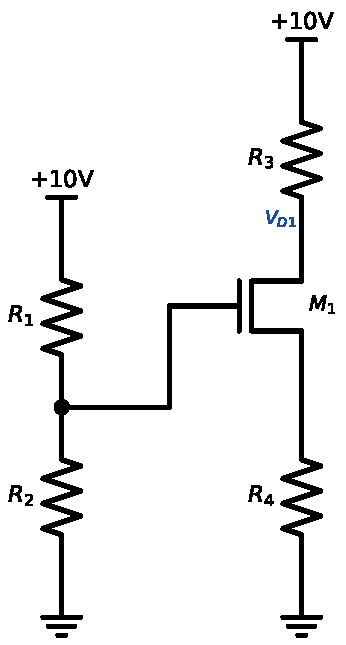
\includegraphics[width=\linewidth,height=6cm,keepaspectratio]{p01_circuit}\end{minipage}\hfill\begin{minipage}{0.38\linewidth}\begin{center}\small\renewcommand{\arraystretch}{1.35}
\begin{tabular}{ll}
\toprule
specification & value \\
\midrule
$I_{D1}$ & $500\,\mu \mathrm{A}$ \\
$V_{D1}$ & $6\,\mathrm{V}$ \\
\bottomrule
\end{tabular}\end{center}
\end{minipage}
\end{probbox}

\begin{probbox}{Problem 5C.2 \hfill Easy}
Design the circuit below: find all resistor values so that the specifications in the table are met with every transistor active. Assume $k'_p\frac{W}{L} = 850\,\mu \mathrm{A/V^2}$, $V_{tp} = -1.3$\,V. Design choices: $V_{R3} = 1.5$\,V; $R_{1}\|R_{2} = 500\,\mathrm{k}\Omega$ (input resistance).

\smallskip\noindent\begin{minipage}{0.6\linewidth}\centering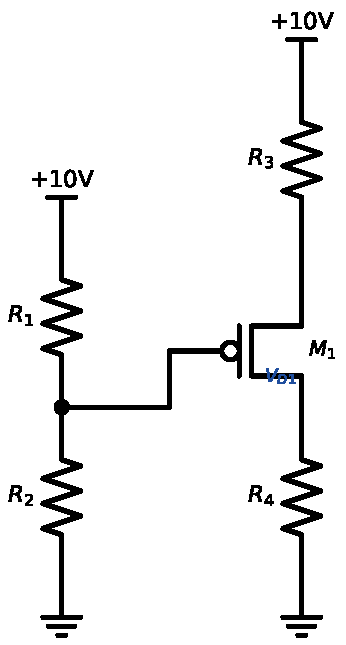
\includegraphics[width=\linewidth,height=6cm,keepaspectratio]{p02_circuit}\end{minipage}\hfill\begin{minipage}{0.38\linewidth}\begin{center}\small\renewcommand{\arraystretch}{1.35}
\begin{tabular}{ll}
\toprule
specification & value \\
\midrule
$I_{D1}$ & $400\,\mu \mathrm{A}$ \\
$V_{D1}$ & $3\,\mathrm{V}$ \\
\bottomrule
\end{tabular}\end{center}
\end{minipage}
\end{probbox}

\begin{probbox}{Problem 5C.3 \hfill Easy}
Design the circuit below: find all resistor values so that the specifications in the table are met with every transistor active. Assume $k'_n\frac{W}{L} = 1.1\,\mathrm{m}\mathrm{A/V^2}$, $V_{tn} = 1.4$\,V. Design choices: divider current $I_{R2} = 20\,\mu \mathrm{A}$.

\smallskip\noindent\begin{minipage}{0.6\linewidth}\centering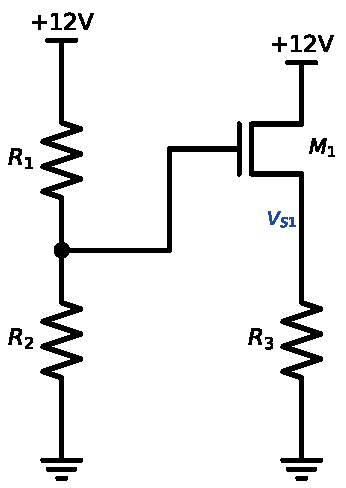
\includegraphics[width=\linewidth,height=6cm,keepaspectratio]{p03_circuit}\end{minipage}\hfill\begin{minipage}{0.38\linewidth}\begin{center}\small\renewcommand{\arraystretch}{1.35}
\begin{tabular}{ll}
\toprule
specification & value \\
\midrule
$I_{D1}$ & $1\,\mathrm{m}\mathrm{A}$ \\
$V_{S1}$ & $4\,\mathrm{V}$ \\
\bottomrule
\end{tabular}\end{center}
\end{minipage}
\end{probbox}

\begin{probbox}{Problem 5C.4 \hfill Easy}
Design the circuit below: find all resistor values so that the specifications in the table are met with every transistor active. Assume $k'_n\frac{W}{L} = 1.1\,\mathrm{m}\mathrm{A/V^2}$, $V_{tn} = 1.4$\,V.

\smallskip\noindent\begin{minipage}{0.6\linewidth}\centering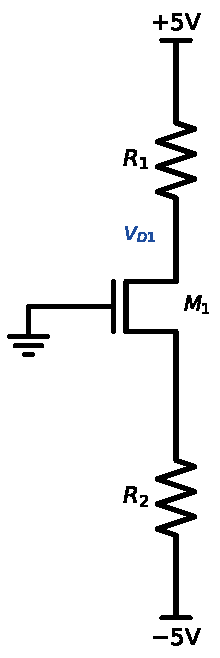
\includegraphics[width=\linewidth,height=6cm,keepaspectratio]{p04_circuit}\end{minipage}\hfill\begin{minipage}{0.38\linewidth}\begin{center}\small\renewcommand{\arraystretch}{1.35}
\begin{tabular}{ll}
\toprule
specification & value \\
\midrule
$I_{D1}$ & $500\,\mu \mathrm{A}$ \\
$V_{D1}$ & $2\,\mathrm{V}$ \\
\bottomrule
\end{tabular}\end{center}
\end{minipage}
\end{probbox}

\begin{probbox}{Problem 5C.5 \hfill Easy}
Design the circuit below: find all resistor values and the width $W$ of every transistor marked ``?'' (keep its length $L$) so that the specifications in the table are met with every transistor active. Assume $k'_n = 200\,\mu \mathrm{A/V^2}$, $V_{tn} = 0.7$\,V (W/L next to each transistor).

\smallskip\noindent\begin{minipage}{0.6\linewidth}\centering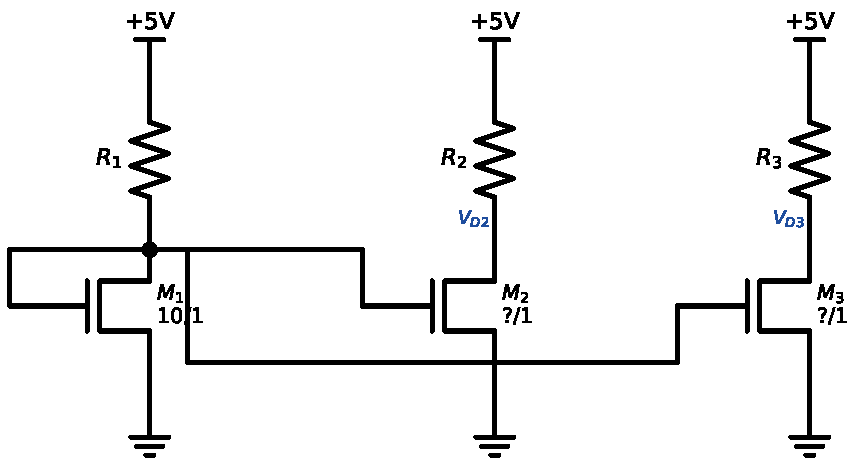
\includegraphics[width=\linewidth,height=6cm,keepaspectratio]{p05_circuit}\end{minipage}\hfill\begin{minipage}{0.38\linewidth}\begin{center}\small\renewcommand{\arraystretch}{1.35}
\begin{tabular}{ll}
\toprule
specification & value \\
\midrule
$I_{D1}$ & $100\,\mu \mathrm{A}$ \\
$I_{D2}$ & $200\,\mu \mathrm{A}$ \\
$I_{D3}$ & $50\,\mu \mathrm{A}$ \\
$V_{D2}$ & $2\,\mathrm{V}$ \\
$V_{D3}$ & $3\,\mathrm{V}$ \\
\bottomrule
\end{tabular}\end{center}
\end{minipage}
\end{probbox}

\begin{probbox}{Problem 5C.6 \hfill Easy}
Design the circuit below: find all resistor values and the width $W$ of every transistor marked ``?'' (keep its length $L$) so that the specifications in the table are met with every transistor active. Assume $k'_p = 100\,\mu \mathrm{A/V^2}$, $V_{tp} = -0.8$\,V (W/L next to each transistor).

\smallskip\noindent\begin{minipage}{0.6\linewidth}\centering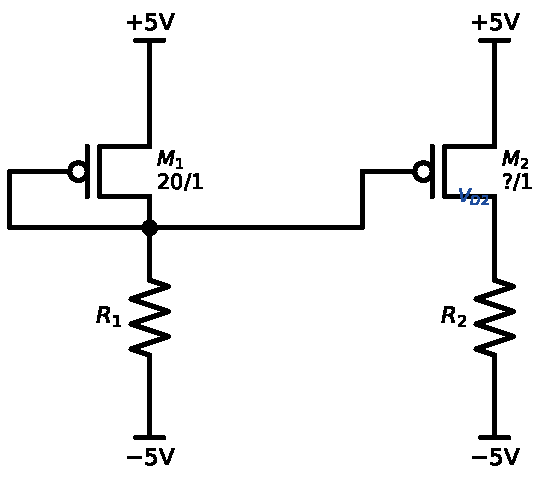
\includegraphics[width=\linewidth,height=6cm,keepaspectratio]{p06_circuit}\end{minipage}\hfill\begin{minipage}{0.38\linewidth}\begin{center}\small\renewcommand{\arraystretch}{1.35}
\begin{tabular}{ll}
\toprule
specification & value \\
\midrule
$I_{D1}$ & $50\,\mu \mathrm{A}$ \\
$I_{D2}$ & $150\,\mu \mathrm{A}$ \\
$V_{D2}$ & $0\,\mathrm{V}$ \\
\bottomrule
\end{tabular}\end{center}
\end{minipage}
\end{probbox}

\subsection*{Medium problems}
\begin{probbox}{Problem 5C.7 \hfill Medium}
Design the circuit below: find all resistor values so that the specifications in the table are met with every transistor active. Assume $k'_n\frac{W}{L} = 1.1\,\mathrm{m}\mathrm{A/V^2}$, $V_{tn} = 1.4$\,V, $k'_p\frac{W}{L} = 850\,\mu \mathrm{A/V^2}$, $V_{tp} = -1.3$\,V. Design choices: $V_{R4} = 1$\,V; $V_{R5} = 2$\,V; divider current $I_{R2} = 5\,\mu \mathrm{A}$.

\smallskip\noindent\begin{minipage}{0.6\linewidth}\centering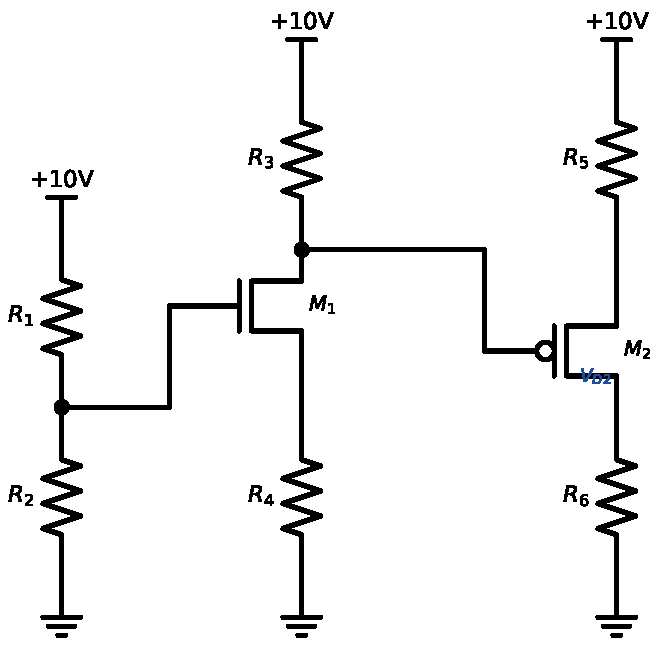
\includegraphics[width=\linewidth,height=6cm,keepaspectratio]{p07_circuit}\end{minipage}\hfill\begin{minipage}{0.38\linewidth}\begin{center}\small\renewcommand{\arraystretch}{1.35}
\begin{tabular}{ll}
\toprule
specification & value \\
\midrule
$I_{D1}$ & $200\,\mu \mathrm{A}$ \\
$I_{D2}$ & $500\,\mu \mathrm{A}$ \\
$V_{D2}$ & $2\,\mathrm{V}$ \\
\bottomrule
\end{tabular}\end{center}
\end{minipage}
\end{probbox}

\begin{probbox}{Problem 5C.8 \hfill Medium}
Design the circuit below: find all resistor values so that the specifications in the table are met with every transistor active. Assume $k'_n\frac{W}{L} = 1.1\,\mathrm{m}\mathrm{A/V^2}$, $V_{tn} = 1.4$\,V. Design choices: $V_{R4} = 1$\,V; $R_{1}\|R_{2} = 1\,\mathrm{M}\Omega$ (input resistance).

\smallskip\noindent\begin{minipage}{0.6\linewidth}\centering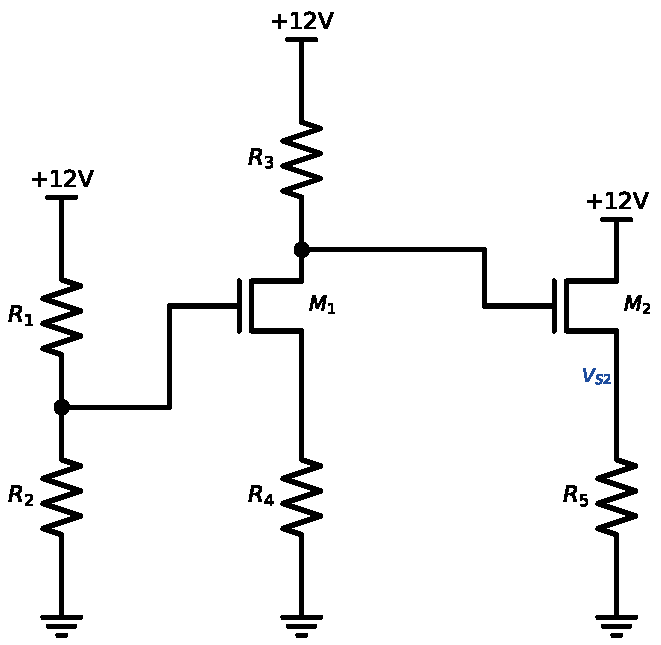
\includegraphics[width=\linewidth,height=6cm,keepaspectratio]{p08_circuit}\end{minipage}\hfill\begin{minipage}{0.38\linewidth}\begin{center}\small\renewcommand{\arraystretch}{1.35}
\begin{tabular}{ll}
\toprule
specification & value \\
\midrule
$I_{D1}$ & $250\,\mu \mathrm{A}$ \\
$I_{D2}$ & $1\,\mathrm{m}\mathrm{A}$ \\
$V_{S2}$ & $5\,\mathrm{V}$ \\
\bottomrule
\end{tabular}\end{center}
\end{minipage}
\end{probbox}

\begin{probbox}{Problem 5C.9 \hfill Medium}
Design the circuit below: find all resistor values so that the specifications in the table are met with every transistor active. Assume $k'_n\frac{W}{L} = 1.1\,\mathrm{m}\mathrm{A/V^2}$, $V_{tn} = 1.4$\,V, $k'_p\frac{W}{L} = 850\,\mu \mathrm{A/V^2}$, $V_{tp} = -1.3$\,V. Design choices: $V_{R3} = 2$\,V; $V_{R6} = 1$\,V; divider current $I_{R2} = 10\,\mu \mathrm{A}$.

\smallskip\noindent\begin{minipage}{0.6\linewidth}\centering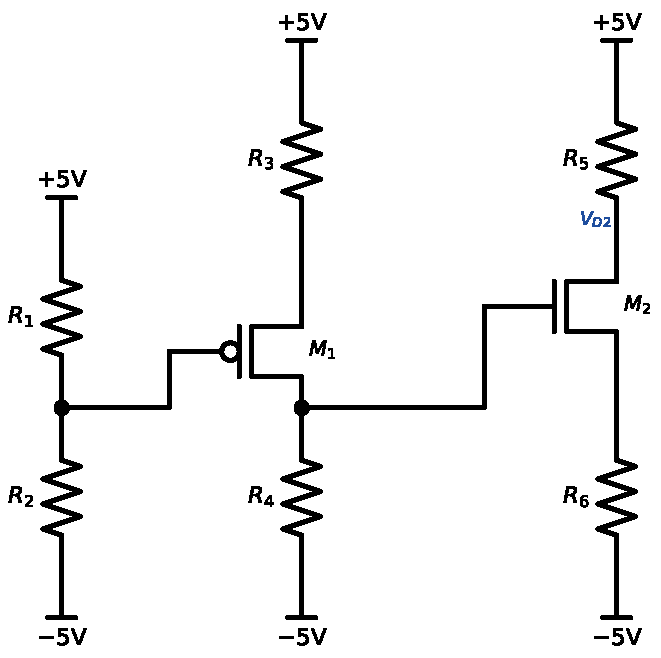
\includegraphics[width=\linewidth,height=6cm,keepaspectratio]{p09_circuit}\end{minipage}\hfill\begin{minipage}{0.38\linewidth}\begin{center}\small\renewcommand{\arraystretch}{1.35}
\begin{tabular}{ll}
\toprule
specification & value \\
\midrule
$I_{D1}$ & $200\,\mu \mathrm{A}$ \\
$I_{D2}$ & $400\,\mu \mathrm{A}$ \\
$V_{D2}$ & $1\,\mathrm{V}$ \\
\bottomrule
\end{tabular}\end{center}
\end{minipage}
\end{probbox}

\begin{probbox}{Problem 5C.10 \hfill Medium}
Design the circuit below: find all resistor values and the width $W$ of every transistor marked ``?'' (keep its length $L$) so that the specifications in the table are met with every transistor active. Assume $k'_n = 200\,\mu \mathrm{A/V^2}$, $V_{tn} = 0.7$\,V (W/L next to each transistor). Design choices: divider current $I_{R3} = 5\,\mu \mathrm{A}$.

\smallskip\noindent\begin{minipage}{0.6\linewidth}\centering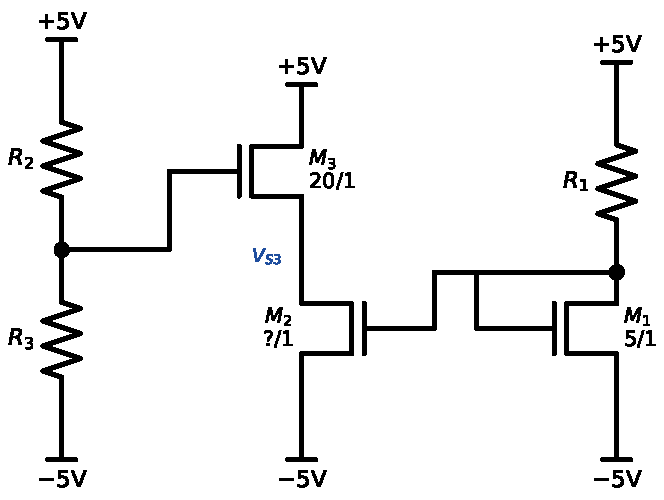
\includegraphics[width=\linewidth,height=6cm,keepaspectratio]{p10_circuit}\end{minipage}\hfill\begin{minipage}{0.38\linewidth}\begin{center}\small\renewcommand{\arraystretch}{1.35}
\begin{tabular}{ll}
\toprule
specification & value \\
\midrule
$I_{D1}$ & $50\,\mu \mathrm{A}$ \\
$I_{D2}$ & $200\,\mu \mathrm{A}$ \\
$V_{S3}$ & $-1\,\mathrm{V}$ \\
\bottomrule
\end{tabular}\end{center}
\end{minipage}
\end{probbox}

\begin{probbox}{Problem 5C.11 \hfill Medium}
Design the circuit below: find all resistor values and the width $W$ of every transistor marked ``?'' (keep its length $L$) so that the specifications in the table are met with every transistor active. Assume $k'_n = 200\,\mu \mathrm{A/V^2}$, $V_{tn} = 0.7$\,V, $k'_p = 100\,\mu \mathrm{A/V^2}$, $V_{tp} = -0.8$\,V (W/L next to each transistor).

\smallskip\noindent\begin{minipage}{0.6\linewidth}\centering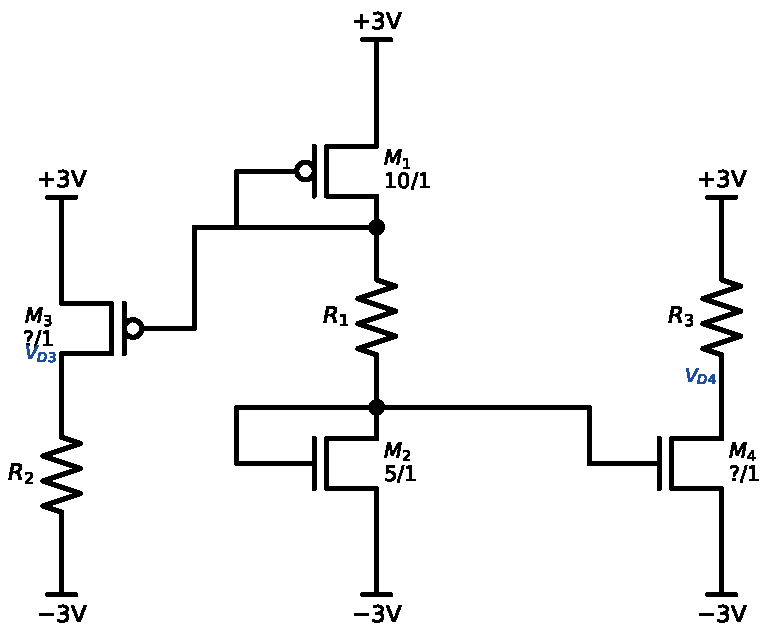
\includegraphics[width=\linewidth,height=6cm,keepaspectratio]{p11_circuit}\end{minipage}\hfill\begin{minipage}{0.38\linewidth}\begin{center}\small\renewcommand{\arraystretch}{1.35}
\begin{tabular}{ll}
\toprule
specification & value \\
\midrule
$I_{D1}$ & $100\,\mu \mathrm{A}$ \\
$I_{D3}$ & $300\,\mu \mathrm{A}$ \\
$I_{D4}$ & $150\,\mu \mathrm{A}$ \\
$V_{D3}$ & $0\,\mathrm{V}$ \\
$V_{D4}$ & $0.5\,\mathrm{V}$ \\
\bottomrule
\end{tabular}\end{center}
\end{minipage}
\end{probbox}

\begin{probbox}{Problem 5C.12 \hfill Medium}
Design the circuit below: find all resistor values so that the specifications in the table are met with every transistor active. Assume $k'_n\frac{W}{L} = 1.1\,\mathrm{m}\mathrm{A/V^2}$, $V_{tn} = 1.4$\,V, $k'_p\frac{W}{L} = 850\,\mu \mathrm{A/V^2}$, $V_{tp} = -1.3$\,V. Design choices: $V_{R3} = 1.5$\,V; divider current $I_{R2} = 20\,\mu \mathrm{A}$.

\smallskip\noindent\begin{minipage}{0.6\linewidth}\centering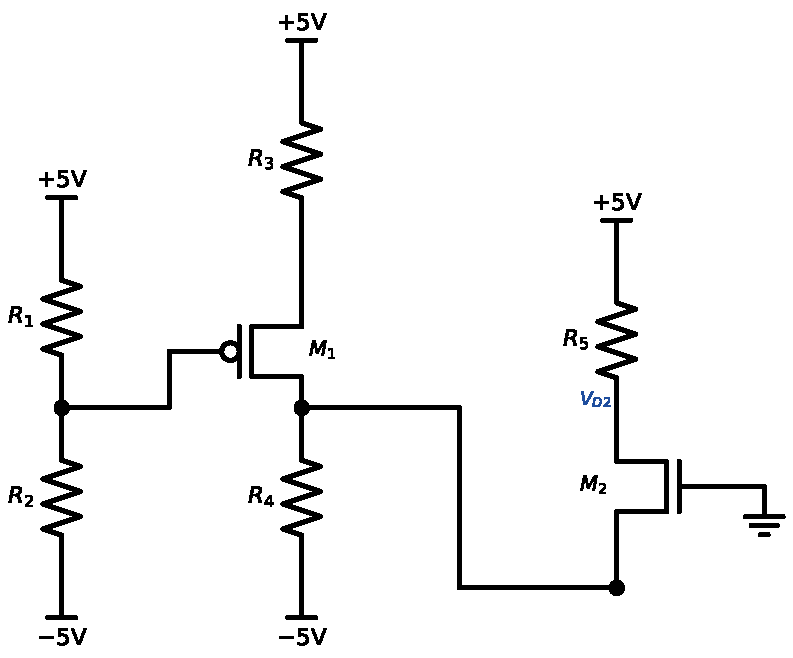
\includegraphics[width=\linewidth,height=6cm,keepaspectratio]{p12_circuit}\end{minipage}\hfill\begin{minipage}{0.38\linewidth}\begin{center}\small\renewcommand{\arraystretch}{1.35}
\begin{tabular}{ll}
\toprule
specification & value \\
\midrule
$I_{D1}$ & $150\,\mu \mathrm{A}$ \\
$I_{D2}$ & $200\,\mu \mathrm{A}$ \\
$V_{D2}$ & $2\,\mathrm{V}$ \\
\bottomrule
\end{tabular}\end{center}
\end{minipage}
\end{probbox}

\subsection*{Hard problems}
\begin{probbox}{Problem 5C.13 \hfill Hard}
Design the circuit below: find all resistor values so that the specifications in the table are met with every transistor active. Assume $k'_n\frac{W}{L} = 1.1\,\mathrm{m}\mathrm{A/V^2}$, $V_{tn} = 1.4$\,V, $k'_p\frac{W}{L} = 850\,\mu \mathrm{A/V^2}$, $V_{tp} = -1.3$\,V. Design choices: $V_{R4} = 1$\,V; $V_{R5} = 2$\,V; $R_{1}\|R_{2} = 500\,\mathrm{k}\Omega$ (input resistance).

\smallskip\noindent\begin{minipage}{0.6\linewidth}\centering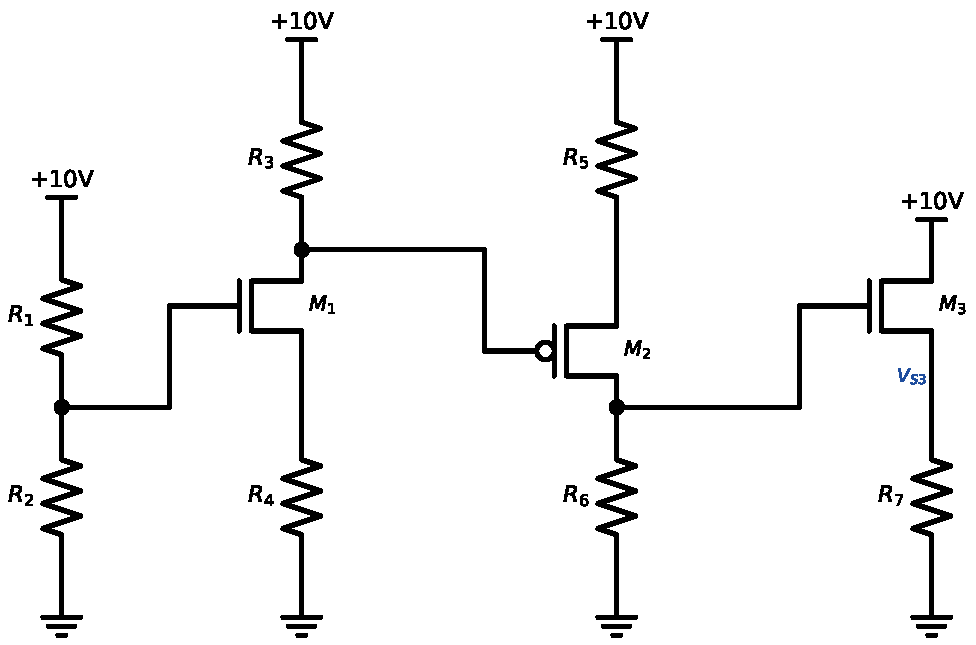
\includegraphics[width=\linewidth,height=6cm,keepaspectratio]{p13_circuit}\end{minipage}\hfill\begin{minipage}{0.38\linewidth}\begin{center}\small\renewcommand{\arraystretch}{1.35}
\begin{tabular}{ll}
\toprule
specification & value \\
\midrule
$I_{D1}$ & $200\,\mu \mathrm{A}$ \\
$I_{D2}$ & $500\,\mu \mathrm{A}$ \\
$I_{D3}$ & $1\,\mathrm{m}\mathrm{A}$ \\
$V_{S3}$ & $4\,\mathrm{V}$ \\
\bottomrule
\end{tabular}\end{center}
\end{minipage}
\end{probbox}

\begin{probbox}{Problem 5C.14 \hfill Hard}
Design the circuit below: find all resistor values so that the specifications in the table are met with every transistor active. Assume $k'_n\frac{W}{L} = 1.1\,\mathrm{m}\mathrm{A/V^2}$, $V_{tn} = 1.4$\,V, $k'_p\frac{W}{L} = 850\,\mu \mathrm{A/V^2}$, $V_{tp} = -1.3$\,V. Design choices: $V_{R3} = 1.5$\,V; $V_{R6} = 1$\,V; divider current $I_{R2} = 20\,\mu \mathrm{A}$.

\smallskip\noindent\begin{minipage}{0.6\linewidth}\centering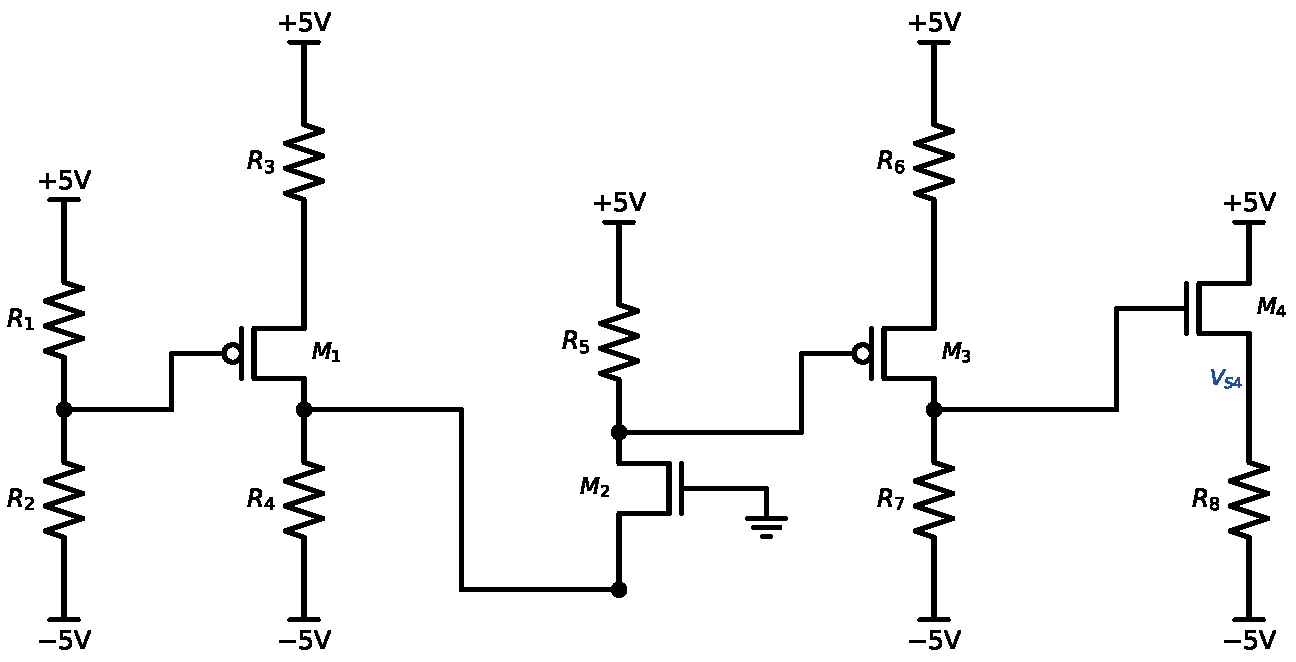
\includegraphics[width=\linewidth,height=6cm,keepaspectratio]{p14_circuit}\end{minipage}\hfill\begin{minipage}{0.38\linewidth}\begin{center}\small\renewcommand{\arraystretch}{1.35}
\begin{tabular}{ll}
\toprule
specification & value \\
\midrule
$I_{D1}$ & $100\,\mu \mathrm{A}$ \\
$I_{D2}$ & $200\,\mu \mathrm{A}$ \\
$I_{D3}$ & $500\,\mu \mathrm{A}$ \\
$I_{D4}$ & $1\,\mathrm{m}\mathrm{A}$ \\
$V_{S4}$ & $-2\,\mathrm{V}$ \\
\bottomrule
\end{tabular}\end{center}
\end{minipage}
\end{probbox}

\begin{probbox}{Problem 5C.15 \hfill Hard}
Design the circuit below: find all resistor values and the width $W$ of every transistor marked ``?'' (keep its length $L$) so that the specifications in the table are met with every transistor active. Assume $k'_n = 200\,\mu \mathrm{A/V^2}$, $V_{tn} = 0.7$\,V, $k'_p = 100\,\mu \mathrm{A/V^2}$, $V_{tp} = -0.8$\,V (W/L next to each transistor).

\smallskip\noindent\begin{minipage}{0.6\linewidth}\centering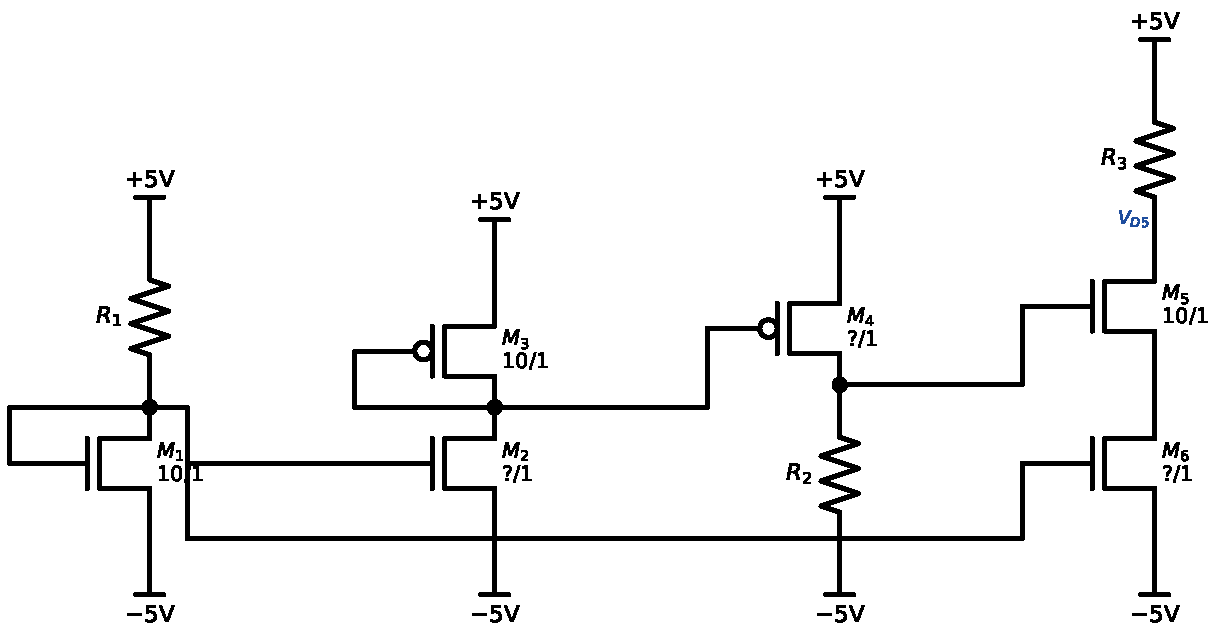
\includegraphics[width=\linewidth,height=6cm,keepaspectratio]{p15_circuit}\end{minipage}\hfill\begin{minipage}{0.38\linewidth}\begin{center}\small\renewcommand{\arraystretch}{1.35}
\begin{tabular}{ll}
\toprule
specification & value \\
\midrule
$I_{D1}$ & $100\,\mu \mathrm{A}$ \\
$I_{D2}$ & $50\,\mu \mathrm{A}$ \\
$I_{D4}$ & $200\,\mu \mathrm{A}$ \\
$I_{D6}$ & $300\,\mu \mathrm{A}$ \\
$V_{D4}$ & $-1\,\mathrm{V}$ \\
$V_{D5}$ & $2\,\mathrm{V}$ \\
\bottomrule
\end{tabular}\end{center}
\end{minipage}
\end{probbox}

\begin{probbox}{Problem 5C.16 \hfill Hard}
Design the circuit below: find all resistor values so that the specifications in the table are met with every transistor active. Assume $k'_n\frac{W}{L} = 1.1\,\mathrm{m}\mathrm{A/V^2}$, $V_{tn} = 1.4$\,V, $k'_p\frac{W}{L} = 850\,\mu \mathrm{A/V^2}$, $V_{tp} = -1.3$\,V. Design choices: $V_{R4} = 1$\,V; $V_{R9} = 1$\,V; divider current $I_{R2} = 10\,\mu \mathrm{A}$; $R_{6}\|R_{7} = 600\,\mathrm{k}\Omega$ (input resistance).

\smallskip\noindent\begin{minipage}{0.6\linewidth}\centering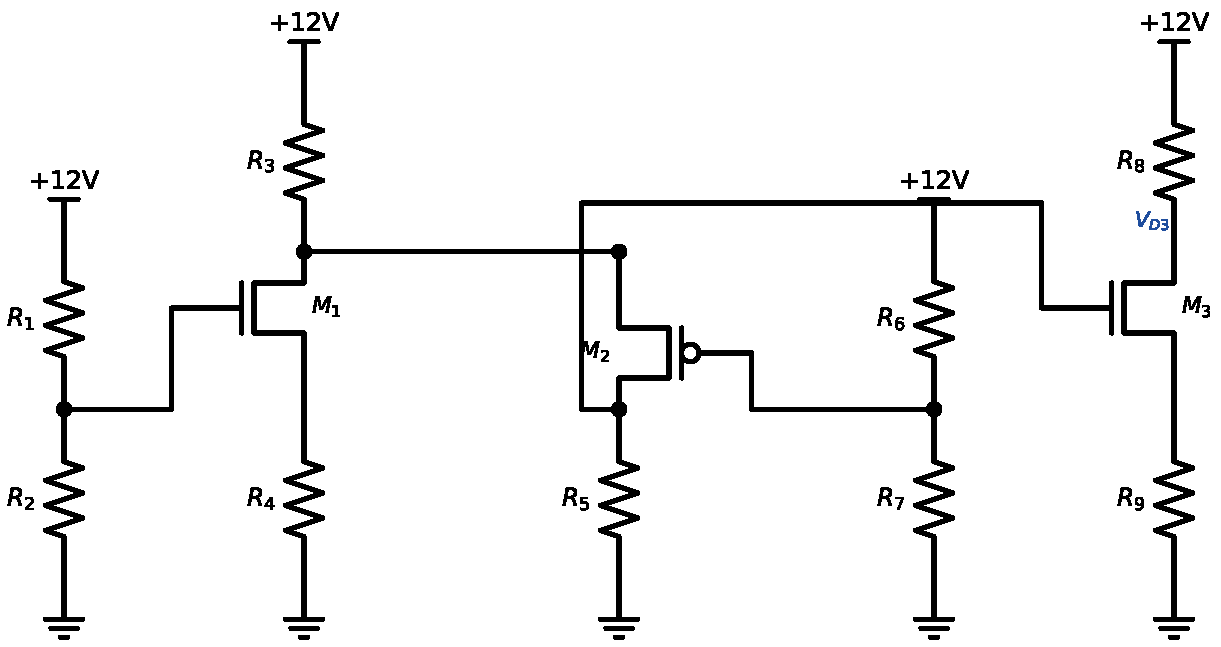
\includegraphics[width=\linewidth,height=6cm,keepaspectratio]{p16_circuit}\end{minipage}\hfill\begin{minipage}{0.38\linewidth}\begin{center}\small\renewcommand{\arraystretch}{1.35}
\begin{tabular}{ll}
\toprule
specification & value \\
\midrule
$I_{D1}$ & $300\,\mu \mathrm{A}$ \\
$I_{D2}$ & $200\,\mu \mathrm{A}$ \\
$I_{D3}$ & $500\,\mu \mathrm{A}$ \\
$V_{D1}$ & $9\,\mathrm{V}$ \\
$V_{D3}$ & $6\,\mathrm{V}$ \\
\bottomrule
\end{tabular}\end{center}
\end{minipage}
\end{probbox}

\begin{probbox}{Problem 5C.17 \hfill Hard}
Design the circuit below: find all resistor values and the width $W$ of every transistor marked ``?'' (keep its length $L$) so that the specifications in the table are met with every transistor active. Assume $k'_n = 200\,\mu \mathrm{A/V^2}$, $V_{tn} = 0.7$\,V, $k'_p = 100\,\mu \mathrm{A/V^2}$, $V_{tp} = -0.8$\,V (W/L next to each transistor).

\smallskip\noindent\begin{minipage}{0.6\linewidth}\centering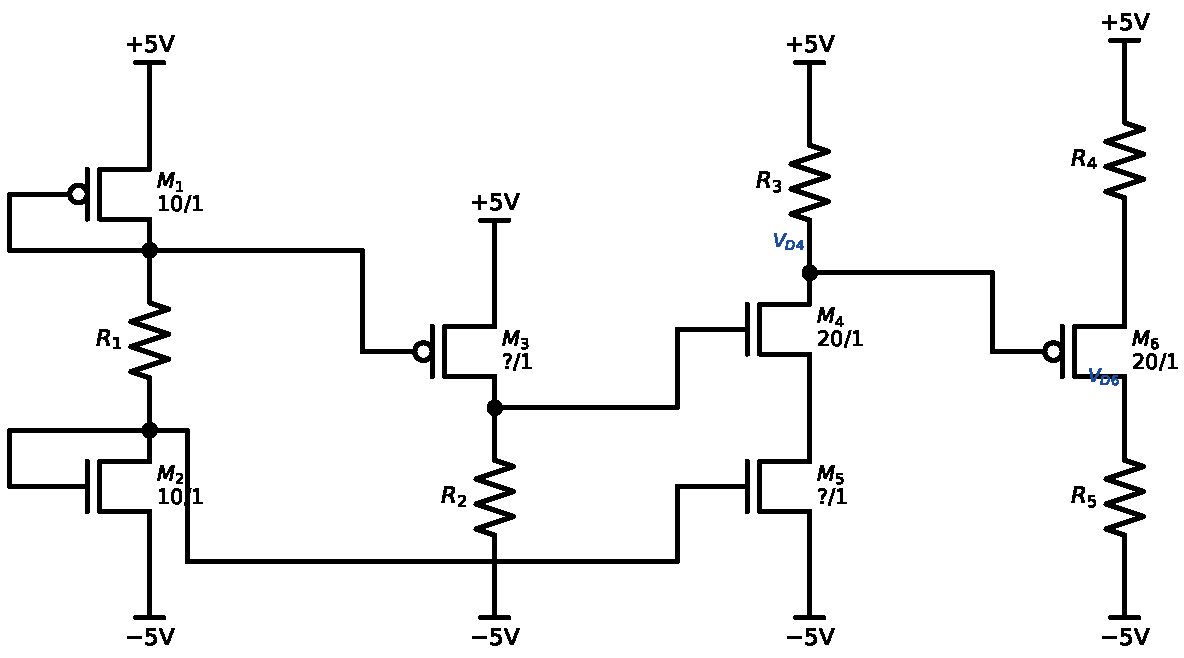
\includegraphics[width=\linewidth,height=6cm,keepaspectratio]{p17_circuit}\end{minipage}\hfill\begin{minipage}{0.38\linewidth}\begin{center}\small\renewcommand{\arraystretch}{1.35}
\begin{tabular}{ll}
\toprule
specification & value \\
\midrule
$I_{D1}$ & $100\,\mu \mathrm{A}$ \\
$I_{D3}$ & $200\,\mu \mathrm{A}$ \\
$I_{D5}$ & $400\,\mu \mathrm{A}$ \\
$I_{D6}$ & $300\,\mu \mathrm{A}$ \\
$V_{D3}$ & $0\,\mathrm{V}$ \\
$V_{D4}$ & $1\,\mathrm{V}$ \\
$V_{D6}$ & $-2\,\mathrm{V}$ \\
\bottomrule
\end{tabular}\end{center}
\end{minipage}
\end{probbox}

\begin{probbox}{Problem 5C.18 \hfill Hard}
Design the circuit below: find all resistor values so that the specifications in the table are met with every transistor active. Assume $k'_n\frac{W}{L} = 1.1\,\mathrm{m}\mathrm{A/V^2}$, $V_{tn} = 1.4$\,V, $k'_p\frac{W}{L} = 850\,\mu \mathrm{A/V^2}$, $V_{tp} = -1.3$\,V. Design choices: $V_{R4} = 1$\,V; $V_{R5} = 1.5$\,V; $V_{R8} = 1$\,V; $V_{R9} = 1.5$\,V; divider current $I_{R2} = 10\,\mu \mathrm{A}$.

\smallskip\noindent\begin{minipage}{0.6\linewidth}\centering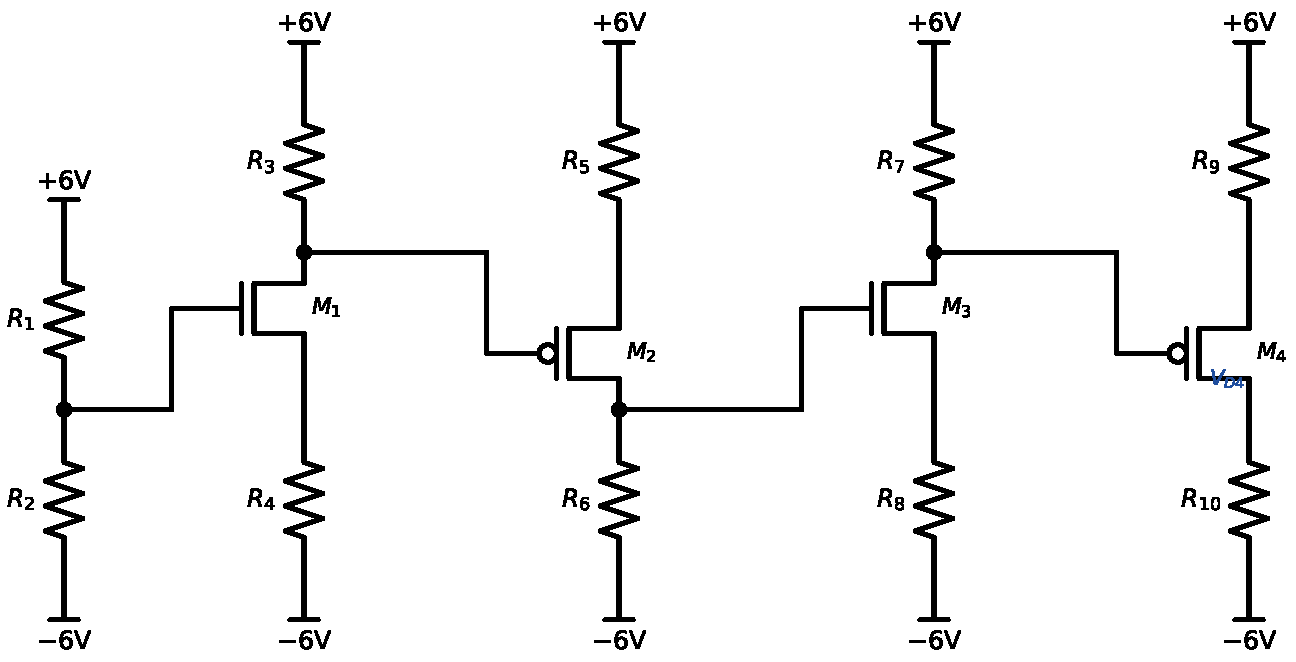
\includegraphics[width=\linewidth,height=6cm,keepaspectratio]{p18_circuit}\end{minipage}\hfill\begin{minipage}{0.38\linewidth}\begin{center}\small\renewcommand{\arraystretch}{1.35}
\begin{tabular}{ll}
\toprule
specification & value \\
\midrule
$I_{D1}$ & $200\,\mu \mathrm{A}$ \\
$I_{D2}$ & $300\,\mu \mathrm{A}$ \\
$I_{D3}$ & $500\,\mu \mathrm{A}$ \\
$I_{D4}$ & $800\,\mu \mathrm{A}$ \\
$V_{D4}$ & $-3\,\mathrm{V}$ \\
\bottomrule
\end{tabular}\end{center}
\end{minipage}
\end{probbox}

\newpage
\section*{Solutions}
Every solution follows the steps of the Lecture-5 pipeline card.
\subsection*{Solution 5C.1 \hfill Easy}
\begin{center}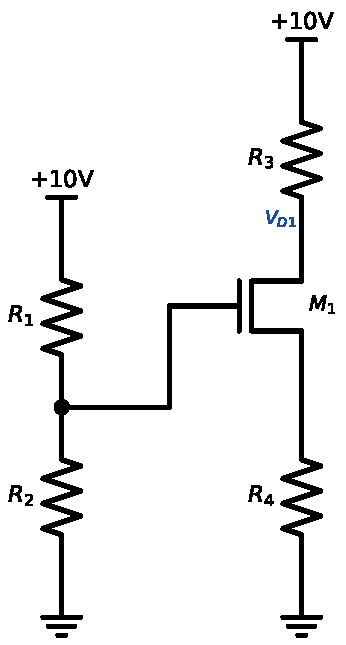
\includegraphics[width=0.9\linewidth,height=6cm,keepaspectratio]{p01_circuit}\end{center}
\solstep{1}{Rules}Run the DC analysis backwards. A target current fixes the gate--source voltage (tool T1): $V_{ov} = \sqrt{2I_D/k}$, $|V_{GS}| = |V_t| + V_{ov}$. A resistor is known as soon as the voltages at both of its ends and its current are known: $R = \Delta V/I$ ($I_G = 0$, so gate dividers carry only their own current). A mirror output copies the reference scaled by $W/L$ (tool T3). Work from the nodes that are already fixed towards the unknown ones.
\solstep{2}{Design, node by node}\begin{enumerate}[leftmargin=*,itemsep=3pt]
\item Design choice: $V_{R4} = 1$\,V across $R_{4}$: $V_{S1} = 0 + 1 = 1\,\mathrm{V}$.
\item Design choice: the divider current is $I_{R2} = 10\,\mu \mathrm{A}$ (any value works for the bias because $I_G = 0$; it only sets the divider resistance).
\item $M_{1}$ must carry $I_{D1} = 500\,\mu \mathrm{A}$: $V_{ov1} = \sqrt{\frac{2I_{D1}}{k_{1}}} = \sqrt{\frac{2\cdot500\,\mu \mathrm{A}}{1.1\,\mathrm{m}\mathrm{A/V^2}}} = 0.9535$\,V, $V_{GS1} = 1.4 + 0.9535 = 2.353$\,V: $V_{G1} = V_{S1} + V_{GS1} = 3.35\,\mathrm{V}$.
\item The only current through $R_{1}$ is $I_{R2} = 10\,\mu \mathrm{A}$ ($I_G = 0$).
\item $\displaystyle R_{1} = \frac{10 - V_{G1}}{I_{R2}} = \frac{10 - 3.353}{10\,\mu \mathrm{A}} = \mathbf{665\,\mathrm{k}\Omega}$
\item $\displaystyle R_{2} = \frac{V_{G1} - 0}{I_{R2}} = \frac{3.353 - 0}{10\,\mu \mathrm{A}} = \mathbf{335\,\mathrm{k}\Omega}$
\item The only current through $R_{3}$ is $I_{D1} = 500\,\mu \mathrm{A}$ ($I_G = 0$).
\item $\displaystyle R_{3} = \frac{10 - V_{D1}}{I_{D1}} = \frac{10 - 6}{500\,\mu \mathrm{A}} = \mathbf{8\,\mathrm{k}\Omega}$
\item The only current through $R_{4}$ is $I_{D1} = 500\,\mu \mathrm{A}$ ($I_G = 0$).
\item $\displaystyle R_{4} = \frac{V_{S1} - 0}{I_{D1}} = \frac{1 - 0}{500\,\mu \mathrm{A}} = \mathbf{2\,\mathrm{k}\Omega}$
\end{enumerate}

\solstep{3}{Designed circuit}\begin{center}\renewcommand{\arraystretch}{1.35}
\begin{tabular}{cc}
\toprule
element & value \\
\midrule
$R_{1}$ & $665\,\mathrm{k}\Omega$ \\
$R_{2}$ & $335\,\mathrm{k}\Omega$ \\
$R_{3}$ & $8\,\mathrm{k}\Omega$ \\
$R_{4}$ & $2\,\mathrm{k}\Omega$ \\
\bottomrule
\end{tabular}\end{center}
\begin{center}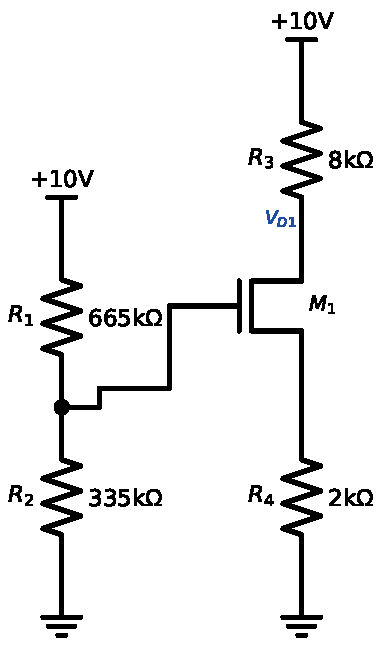
\includegraphics[width=0.85\linewidth,height=6cm,keepaspectratio]{p01_designed}\end{center}

\solstep{4}{Check by analysis}Analyse the finished circuit as in set 5A (one quadratic per transistor, mirrors by $W/L$):\begin{center}\renewcommand{\arraystretch}{1.35}
\begin{tabular}{ccc}
\toprule
 & target $I_D$ & analysis $I_D$ \\
\midrule
$M_{1}$ & $500\,\mu \mathrm{A}$ & $500\,\mu \mathrm{A}$ \\
\bottomrule
\end{tabular}\end{center}
\begin{itemize}[leftmargin=*,itemsep=2pt]
\item $V_{DS1} = V_{D1} - V_{S1} = 6 - 1 = 5\,\mathrm{V}$ $\ge V_{ov1} = 0.953$\,V $\Rightarrow$ $M_{1}$ is active \checkmark
\end{itemize}
Every specified current and voltage is reproduced exactly ($I_G = 0$: nothing was neglected).
\begin{ansbox}
$R_{1} = 665\,\mathrm{k}\Omega$,\quad $R_{2} = 335\,\mathrm{k}\Omega$,\quad $R_{3} = 8\,\mathrm{k}\Omega$,\quad $R_{4} = 2\,\mathrm{k}\Omega$
\end{ansbox}

\newpage
\subsection*{Solution 5C.2 \hfill Easy}
\begin{center}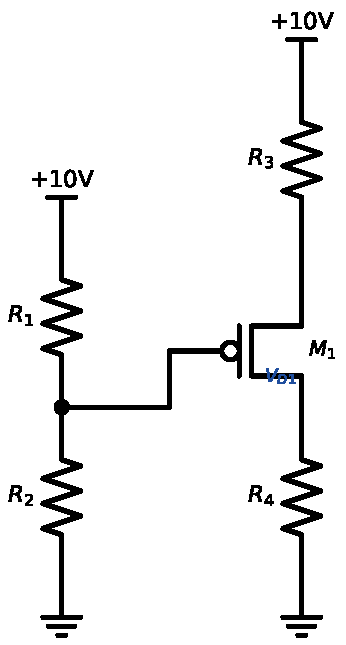
\includegraphics[width=0.9\linewidth,height=6cm,keepaspectratio]{p02_circuit}\end{center}
\solstep{1}{Rules}Run the DC analysis backwards. A target current fixes the gate--source voltage (tool T1): $V_{ov} = \sqrt{2I_D/k}$, $|V_{GS}| = |V_t| + V_{ov}$. A resistor is known as soon as the voltages at both of its ends and its current are known: $R = \Delta V/I$ ($I_G = 0$, so gate dividers carry only their own current). A mirror output copies the reference scaled by $W/L$ (tool T3). Work from the nodes that are already fixed towards the unknown ones.
\solstep{2}{Design, node by node}\begin{enumerate}[leftmargin=*,itemsep=3pt]
\item Design choice: $V_{R3} = 1.5$\,V across $R_{3}$: $V_{S1} = 10 - 1.5 = 8.5\,\mathrm{V}$.
\item $M_{1}$ must carry $I_{D1} = 400\,\mu \mathrm{A}$: $V_{ov1} = \sqrt{\frac{2I_{D1}}{k_{1}}} = \sqrt{\frac{2\cdot400\,\mu \mathrm{A}}{850\,\mu \mathrm{A/V^2}}} = 0.9701$\,V, $V_{SG1} = 1.3 + 0.9701 = 2.27$\,V: $V_{G1} = V_{S1} - V_{SG1} = 6.23\,\mathrm{V}$.
\item Input-resistance requirement: $R_{1}\|R_{2} = 500\,\mathrm{k}\Omega$. Both resistors carry the same current $I$ ($I_G = 0$), so $R_{1} = V_{R1}/I = 3.77X$ and $R_{2} = 6.23X$ with $X = 1/I$. Then $R_{1}\|R_{2} = \frac{3.77\cdot6.23}{10}X = 500\,\mathrm{k}\Omega$ gives $X = 213\,\mathrm{k}\Omega$: $\mathbf{R_{1} = 803\,\mathrm{k}\Omega}$, $\mathbf{R_{2} = 1.33\,\mathrm{M}\Omega}$.
\item The only current through $R_{3}$ is $I_{D1} = 400\,\mu \mathrm{A}$ ($I_G = 0$).
\item $\displaystyle R_{3} = \frac{10 - V_{S1}}{I_{D1}} = \frac{10 - 8.5}{400\,\mu \mathrm{A}} = \mathbf{3.75\,\mathrm{k}\Omega}$
\item The only current through $R_{4}$ is $I_{D1} = 400\,\mu \mathrm{A}$ ($I_G = 0$).
\item $\displaystyle R_{4} = \frac{V_{D1} - 0}{I_{D1}} = \frac{3 - 0}{400\,\mu \mathrm{A}} = \mathbf{7.5\,\mathrm{k}\Omega}$
\end{enumerate}

\solstep{3}{Designed circuit}\begin{center}\renewcommand{\arraystretch}{1.35}
\begin{tabular}{cc}
\toprule
element & value \\
\midrule
$R_{1}$ & $803\,\mathrm{k}\Omega$ \\
$R_{2}$ & $1.33\,\mathrm{M}\Omega$ \\
$R_{3}$ & $3.75\,\mathrm{k}\Omega$ \\
$R_{4}$ & $7.5\,\mathrm{k}\Omega$ \\
\bottomrule
\end{tabular}\end{center}
\begin{center}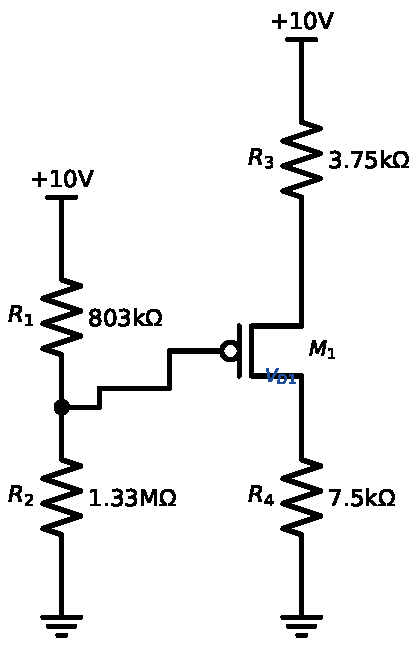
\includegraphics[width=0.85\linewidth,height=6cm,keepaspectratio]{p02_designed}\end{center}

\solstep{4}{Check by analysis}Analyse the finished circuit as in set 5A (one quadratic per transistor, mirrors by $W/L$):\begin{center}\renewcommand{\arraystretch}{1.35}
\begin{tabular}{ccc}
\toprule
 & target $I_D$ & analysis $I_D$ \\
\midrule
$M_{1}$ & $400\,\mu \mathrm{A}$ & $400\,\mu \mathrm{A}$ \\
\bottomrule
\end{tabular}\end{center}
\begin{itemize}[leftmargin=*,itemsep=2pt]
\item $V_{SD1} = V_{S1} - V_{D1} = 8.5 - 3 = 5.5\,\mathrm{V}$ $\ge V_{ov1} = 0.97$\,V $\Rightarrow$ $M_{1}$ is active \checkmark
\end{itemize}
Every specified current and voltage is reproduced exactly ($I_G = 0$: nothing was neglected).
\begin{ansbox}
$R_{1} = 803\,\mathrm{k}\Omega$,\quad $R_{2} = 1.33\,\mathrm{M}\Omega$,\quad $R_{3} = 3.75\,\mathrm{k}\Omega$,\quad $R_{4} = 7.5\,\mathrm{k}\Omega$
\end{ansbox}

\newpage
\subsection*{Solution 5C.3 \hfill Easy}
\begin{center}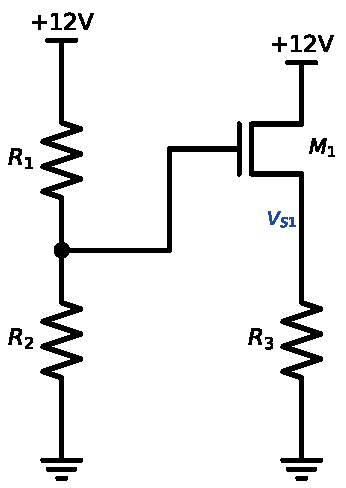
\includegraphics[width=0.9\linewidth,height=6cm,keepaspectratio]{p03_circuit}\end{center}
\solstep{1}{Rules}Run the DC analysis backwards. A target current fixes the gate--source voltage (tool T1): $V_{ov} = \sqrt{2I_D/k}$, $|V_{GS}| = |V_t| + V_{ov}$. A resistor is known as soon as the voltages at both of its ends and its current are known: $R = \Delta V/I$ ($I_G = 0$, so gate dividers carry only their own current). A mirror output copies the reference scaled by $W/L$ (tool T3). Work from the nodes that are already fixed towards the unknown ones.
\solstep{2}{Design, node by node}\begin{enumerate}[leftmargin=*,itemsep=3pt]
\item Design choice: the divider current is $I_{R2} = 20\,\mu \mathrm{A}$ (any value works for the bias because $I_G = 0$; it only sets the divider resistance).
\item $M_{1}$ must carry $I_{D1} = 1\,\mathrm{m}\mathrm{A}$: $V_{ov1} = \sqrt{\frac{2I_{D1}}{k_{1}}} = \sqrt{\frac{2\cdot1\,\mathrm{m}\mathrm{A}}{1.1\,\mathrm{m}\mathrm{A/V^2}}} = 1.348$\,V, $V_{GS1} = 1.4 + 1.348 = 2.748$\,V: $V_{G1} = V_{S1} + V_{GS1} = 6.75\,\mathrm{V}$.
\item The only current through $R_{1}$ is $I_{R2} = 20\,\mu \mathrm{A}$ ($I_G = 0$).
\item $\displaystyle R_{1} = \frac{12 - V_{G1}}{I_{R2}} = \frac{12 - 6.748}{20\,\mu \mathrm{A}} = \mathbf{263\,\mathrm{k}\Omega}$
\item $\displaystyle R_{2} = \frac{V_{G1} - 0}{I_{R2}} = \frac{6.748 - 0}{20\,\mu \mathrm{A}} = \mathbf{337\,\mathrm{k}\Omega}$
\item The only current through $R_{3}$ is $I_{D1} = 1\,\mathrm{m}\mathrm{A}$ ($I_G = 0$).
\item $\displaystyle R_{3} = \frac{V_{S1} - 0}{I_{D1}} = \frac{4 - 0}{1\,\mathrm{m}\mathrm{A}} = \mathbf{4\,\mathrm{k}\Omega}$
\end{enumerate}

\solstep{3}{Designed circuit}\begin{center}\renewcommand{\arraystretch}{1.35}
\begin{tabular}{cc}
\toprule
element & value \\
\midrule
$R_{1}$ & $263\,\mathrm{k}\Omega$ \\
$R_{2}$ & $337\,\mathrm{k}\Omega$ \\
$R_{3}$ & $4\,\mathrm{k}\Omega$ \\
\bottomrule
\end{tabular}\end{center}
\begin{center}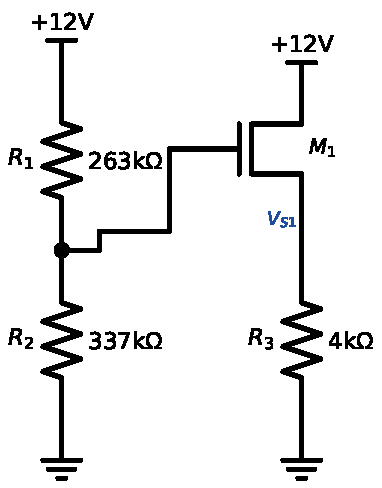
\includegraphics[width=0.85\linewidth,height=6cm,keepaspectratio]{p03_designed}\end{center}

\solstep{4}{Check by analysis}Analyse the finished circuit as in set 5A (one quadratic per transistor, mirrors by $W/L$):\begin{center}\renewcommand{\arraystretch}{1.35}
\begin{tabular}{ccc}
\toprule
 & target $I_D$ & analysis $I_D$ \\
\midrule
$M_{1}$ & $1\,\mathrm{m}\mathrm{A}$ & $1\,\mathrm{m}\mathrm{A}$ \\
\bottomrule
\end{tabular}\end{center}
\begin{itemize}[leftmargin=*,itemsep=2pt]
\item $V_{DS1} = 12 - V_{S1} = 12 - 4 = 8\,\mathrm{V}$ $\ge V_{ov1} = 1.35$\,V $\Rightarrow$ $M_{1}$ is active \checkmark
\end{itemize}
Every specified current and voltage is reproduced exactly ($I_G = 0$: nothing was neglected).
\begin{ansbox}
$R_{1} = 263\,\mathrm{k}\Omega$,\quad $R_{2} = 337\,\mathrm{k}\Omega$,\quad $R_{3} = 4\,\mathrm{k}\Omega$
\end{ansbox}

\newpage
\subsection*{Solution 5C.4 \hfill Easy}
\begin{center}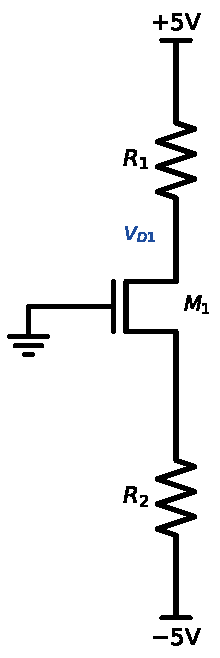
\includegraphics[width=0.9\linewidth,height=6cm,keepaspectratio]{p04_circuit}\end{center}
\solstep{1}{Rules}Run the DC analysis backwards. A target current fixes the gate--source voltage (tool T1): $V_{ov} = \sqrt{2I_D/k}$, $|V_{GS}| = |V_t| + V_{ov}$. A resistor is known as soon as the voltages at both of its ends and its current are known: $R = \Delta V/I$ ($I_G = 0$, so gate dividers carry only their own current). A mirror output copies the reference scaled by $W/L$ (tool T3). Work from the nodes that are already fixed towards the unknown ones.
\solstep{2}{Design, node by node}\begin{enumerate}[leftmargin=*,itemsep=3pt]
\item $M_{1}$ must carry $I_{D1} = 500\,\mu \mathrm{A}$: $V_{ov1} = \sqrt{\frac{2I_{D1}}{k_{1}}} = \sqrt{\frac{2\cdot500\,\mu \mathrm{A}}{1.1\,\mathrm{m}\mathrm{A/V^2}}} = 0.9535$\,V, $V_{GS1} = 1.4 + 0.9535 = 2.353$\,V: $V_{S1} = 0 - V_{GS1} = -2.35\,\mathrm{V}$.
\item The only current through $R_{1}$ is $I_{D1} = 500\,\mu \mathrm{A}$ ($I_G = 0$).
\item $\displaystyle R_{1} = \frac{5 - V_{D1}}{I_{D1}} = \frac{5 - 2}{500\,\mu \mathrm{A}} = \mathbf{6\,\mathrm{k}\Omega}$
\item The only current through $R_{2}$ is $I_{D1} = 500\,\mu \mathrm{A}$ ($I_G = 0$).
\item $\displaystyle R_{2} = \frac{V_{S1} - (-5)}{I_{D1}} = \frac{-2.353 - (-5)}{500\,\mu \mathrm{A}} = \mathbf{5.29\,\mathrm{k}\Omega}$
\end{enumerate}

\solstep{3}{Designed circuit}\begin{center}\renewcommand{\arraystretch}{1.35}
\begin{tabular}{cc}
\toprule
element & value \\
\midrule
$R_{1}$ & $6\,\mathrm{k}\Omega$ \\
$R_{2}$ & $5.29\,\mathrm{k}\Omega$ \\
\bottomrule
\end{tabular}\end{center}
\begin{center}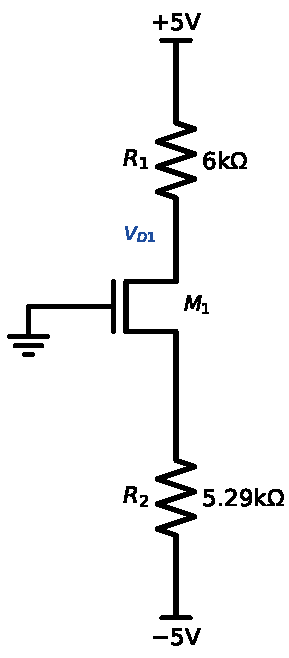
\includegraphics[width=0.85\linewidth,height=6cm,keepaspectratio]{p04_designed}\end{center}

\solstep{4}{Check by analysis}Analyse the finished circuit as in set 5A (one quadratic per transistor, mirrors by $W/L$):\begin{center}\renewcommand{\arraystretch}{1.35}
\begin{tabular}{ccc}
\toprule
 & target $I_D$ & analysis $I_D$ \\
\midrule
$M_{1}$ & $500\,\mu \mathrm{A}$ & $500\,\mu \mathrm{A}$ \\
\bottomrule
\end{tabular}\end{center}
\begin{itemize}[leftmargin=*,itemsep=2pt]
\item $V_{DS1} = V_{D1} - V_{S1} = 2 - (-2.353) = 4.35\,\mathrm{V}$ $\ge V_{ov1} = 0.953$\,V $\Rightarrow$ $M_{1}$ is active \checkmark
\end{itemize}
Every specified current and voltage is reproduced exactly ($I_G = 0$: nothing was neglected).
\begin{ansbox}
$R_{1} = 6\,\mathrm{k}\Omega$,\quad $R_{2} = 5.29\,\mathrm{k}\Omega$
\end{ansbox}

\newpage
\subsection*{Solution 5C.5 \hfill Easy}
\begin{center}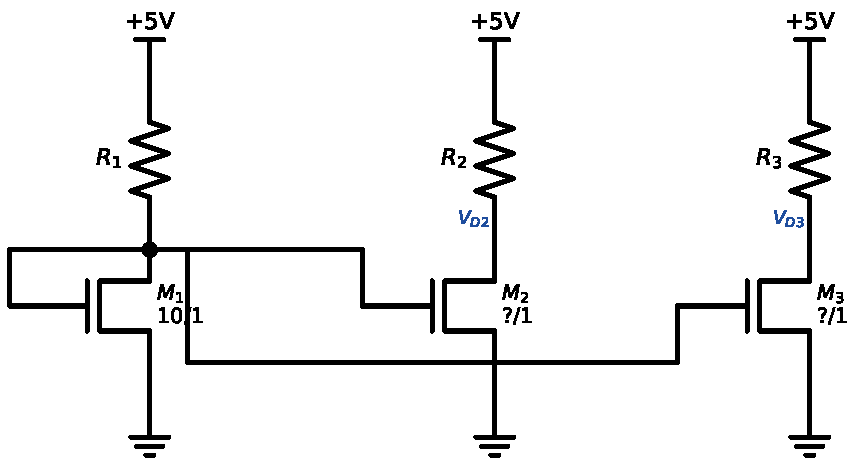
\includegraphics[width=0.9\linewidth,height=6cm,keepaspectratio]{p05_circuit}\end{center}
\solstep{1}{Rules}Run the DC analysis backwards. A target current fixes the gate--source voltage (tool T1): $V_{ov} = \sqrt{2I_D/k}$, $|V_{GS}| = |V_t| + V_{ov}$. A resistor is known as soon as the voltages at both of its ends and its current are known: $R = \Delta V/I$ ($I_G = 0$, so gate dividers carry only their own current). A mirror output copies the reference scaled by $W/L$ (tool T3). Work from the nodes that are already fixed towards the unknown ones.
\solstep{2}{Design, node by node}\begin{enumerate}[leftmargin=*,itemsep=3pt]
\item $M_{2}$ shares gate and source with $M_{1}$ (same $V_{GS}$), so its current scales with $W/L$: $\left(\frac{W}{L}\right)_{2} = \frac{I_{D2}}{I_{D1}}\left(\frac{W}{L}\right)_{1} = \frac{200\,\mu \mathrm{A}}{100\,\mu \mathrm{A}}\cdot\frac{10}{1} = \mathbf{20/1}$ (keep $L = 1\,\mu$m).
\item $M_{3}$ shares gate and source with $M_{1}$ (same $V_{GS}$), so its current scales with $W/L$: $\left(\frac{W}{L}\right)_{3} = \frac{I_{D3}}{I_{D1}}\left(\frac{W}{L}\right)_{1} = \frac{50\,\mu \mathrm{A}}{100\,\mu \mathrm{A}}\cdot\frac{10}{1} = \mathbf{5/1}$ (keep $L = 1\,\mu$m).
\item $M_{1}$ must carry $I_{D1} = 100\,\mu \mathrm{A}$: $V_{ov1} = \sqrt{\frac{2I_{D1}}{k_{1}}} = \sqrt{\frac{2\cdot100\,\mu \mathrm{A}}{2\,\mathrm{m}\mathrm{A/V^2}}} = 0.3162$\,V, $V_{GS1} = 0.7 + 0.3162 = 1.016$\,V: $V_{G1} = 0 + V_{GS1} = 1.02\,\mathrm{V}$ (diode-connected: also its drain).
\item The only current through $R_{1}$ is $I_{D1} = 100\,\mu \mathrm{A}$ ($I_G = 0$).
\item $\displaystyle R_{1} = \frac{5 - V_{G1}}{I_{D1}} = \frac{5 - 1.016}{100\,\mu \mathrm{A}} = \mathbf{39.8\,\mathrm{k}\Omega}$
\item The only current through $R_{2}$ is $I_{D2} = 200\,\mu \mathrm{A}$ ($I_G = 0$).
\item $\displaystyle R_{2} = \frac{5 - V_{D2}}{I_{D2}} = \frac{5 - 2}{200\,\mu \mathrm{A}} = \mathbf{15\,\mathrm{k}\Omega}$
\item The only current through $R_{3}$ is $I_{D3} = 50\,\mu \mathrm{A}$ ($I_G = 0$).
\item $\displaystyle R_{3} = \frac{5 - V_{D3}}{I_{D3}} = \frac{5 - 3}{50\,\mu \mathrm{A}} = \mathbf{40\,\mathrm{k}\Omega}$
\end{enumerate}

\solstep{3}{Designed circuit}\begin{center}\renewcommand{\arraystretch}{1.35}
\begin{tabular}{cc}
\toprule
element & value \\
\midrule
$R_{1}$ & $39.8\,\mathrm{k}\Omega$ \\
$R_{2}$ & $15\,\mathrm{k}\Omega$ \\
$R_{3}$ & $40\,\mathrm{k}\Omega$ \\
$(W/L)_{2}$ & $20/1$ \\
$(W/L)_{3}$ & $5/1$ \\
\bottomrule
\end{tabular}\end{center}
\begin{center}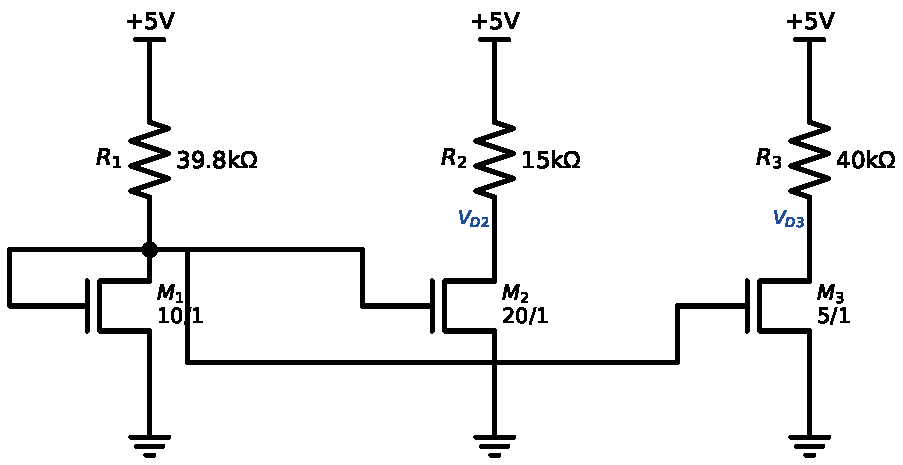
\includegraphics[width=0.85\linewidth,height=6cm,keepaspectratio]{p05_designed}\end{center}

\solstep{4}{Check by analysis}Analyse the finished circuit as in set 5A (one quadratic per transistor, mirrors by $W/L$):\begin{center}\renewcommand{\arraystretch}{1.35}
\begin{tabular}{ccc}
\toprule
 & target $I_D$ & analysis $I_D$ \\
\midrule
$M_{1}$ & $100\,\mu \mathrm{A}$ & $100\,\mu \mathrm{A}$ \\
$M_{2}$ & $200\,\mu \mathrm{A}$ & $200\,\mu \mathrm{A}$ \\
$M_{3}$ & $50\,\mu \mathrm{A}$ & $50\,\mu \mathrm{A}$ \\
\bottomrule
\end{tabular}\end{center}
\begin{itemize}[leftmargin=*,itemsep=2pt]
\item $M_{1}$ is diode-connected: $V_{DS1} = V_{GS1} > V_{ov1}$, always active \checkmark
\item $V_{DS2} = V_{D2} - 0 = 2 - 0 = 2\,\mathrm{V}$ $\ge V_{ov2} = 0.316$\,V $\Rightarrow$ $M_{2}$ is active \checkmark
\item $V_{DS3} = V_{D3} - 0 = 3 - 0 = 3\,\mathrm{V}$ $\ge V_{ov3} = 0.316$\,V $\Rightarrow$ $M_{3}$ is active \checkmark
\end{itemize}
Every specified current and voltage is reproduced exactly ($I_G = 0$: nothing was neglected).
\begin{ansbox}
$R_{1} = 39.8\,\mathrm{k}\Omega$,\quad $R_{2} = 15\,\mathrm{k}\Omega$,\quad $R_{3} = 40\,\mathrm{k}\Omega$,\quad $(W/L)_{2} = 20/1$,\quad $(W/L)_{3} = 5/1$
\end{ansbox}

\newpage
\subsection*{Solution 5C.6 \hfill Easy}
\begin{center}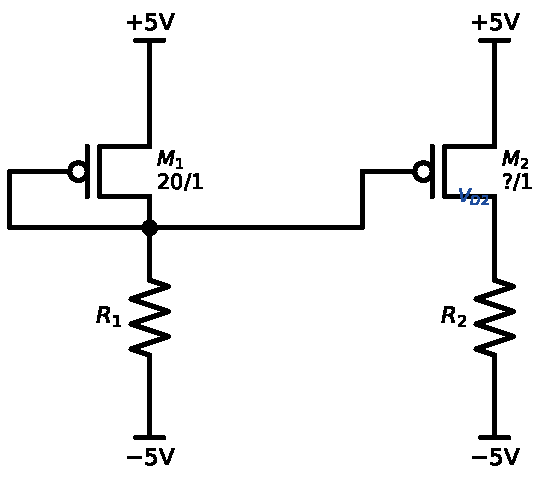
\includegraphics[width=0.9\linewidth,height=6cm,keepaspectratio]{p06_circuit}\end{center}
\solstep{1}{Rules}Run the DC analysis backwards. A target current fixes the gate--source voltage (tool T1): $V_{ov} = \sqrt{2I_D/k}$, $|V_{GS}| = |V_t| + V_{ov}$. A resistor is known as soon as the voltages at both of its ends and its current are known: $R = \Delta V/I$ ($I_G = 0$, so gate dividers carry only their own current). A mirror output copies the reference scaled by $W/L$ (tool T3). Work from the nodes that are already fixed towards the unknown ones.
\solstep{2}{Design, node by node}\begin{enumerate}[leftmargin=*,itemsep=3pt]
\item $M_{2}$ shares gate and source with $M_{1}$ (same $V_{GS}$), so its current scales with $W/L$: $\left(\frac{W}{L}\right)_{2} = \frac{I_{D2}}{I_{D1}}\left(\frac{W}{L}\right)_{1} = \frac{150\,\mu \mathrm{A}}{50\,\mu \mathrm{A}}\cdot\frac{20}{1} = \mathbf{60/1}$ (keep $L = 1\,\mu$m).
\item $M_{1}$ must carry $I_{D1} = 50\,\mu \mathrm{A}$: $V_{ov1} = \sqrt{\frac{2I_{D1}}{k_{1}}} = \sqrt{\frac{2\cdot50\,\mu \mathrm{A}}{2\,\mathrm{m}\mathrm{A/V^2}}} = 0.2236$\,V, $V_{SG1} = 0.8 + 0.2236 = 1.024$\,V: $V_{G1} = 5 - V_{SG1} = 3.98\,\mathrm{V}$ (diode-connected: also its drain).
\item The only current through $R_{1}$ is $I_{D1} = 50\,\mu \mathrm{A}$ ($I_G = 0$).
\item $\displaystyle R_{1} = \frac{V_{G1} - (-5)}{I_{D1}} = \frac{3.976 - (-5)}{50\,\mu \mathrm{A}} = \mathbf{180\,\mathrm{k}\Omega}$
\item The only current through $R_{2}$ is $I_{D2} = 150\,\mu \mathrm{A}$ ($I_G = 0$).
\item $\displaystyle R_{2} = \frac{V_{D2} - (-5)}{I_{D2}} = \frac{0 - (-5)}{150\,\mu \mathrm{A}} = \mathbf{33.3\,\mathrm{k}\Omega}$
\end{enumerate}

\solstep{3}{Designed circuit}\begin{center}\renewcommand{\arraystretch}{1.35}
\begin{tabular}{cc}
\toprule
element & value \\
\midrule
$R_{1}$ & $180\,\mathrm{k}\Omega$ \\
$R_{2}$ & $33.3\,\mathrm{k}\Omega$ \\
$(W/L)_{2}$ & $60/1$ \\
\bottomrule
\end{tabular}\end{center}
\begin{center}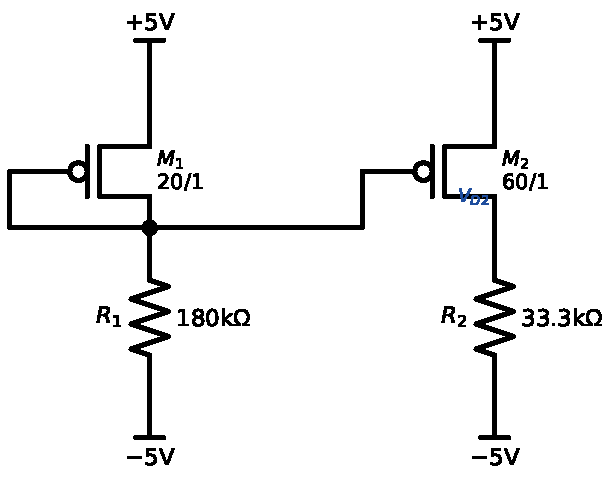
\includegraphics[width=0.85\linewidth,height=6cm,keepaspectratio]{p06_designed}\end{center}

\solstep{4}{Check by analysis}Analyse the finished circuit as in set 5A (one quadratic per transistor, mirrors by $W/L$):\begin{center}\renewcommand{\arraystretch}{1.35}
\begin{tabular}{ccc}
\toprule
 & target $I_D$ & analysis $I_D$ \\
\midrule
$M_{1}$ & $50\,\mu \mathrm{A}$ & $50\,\mu \mathrm{A}$ \\
$M_{2}$ & $150\,\mu \mathrm{A}$ & $150\,\mu \mathrm{A}$ \\
\bottomrule
\end{tabular}\end{center}
\begin{itemize}[leftmargin=*,itemsep=2pt]
\item $M_{1}$ is diode-connected: $V_{SD1} = V_{SG1} > V_{ov1}$, always active \checkmark
\item $V_{SD2} = 5 - V_{D2} = 5 - (-2.078\times 10^{-14}) = 5\,\mathrm{V}$ $\ge V_{ov2} = 0.224$\,V $\Rightarrow$ $M_{2}$ is active \checkmark
\end{itemize}
Every specified current and voltage is reproduced exactly ($I_G = 0$: nothing was neglected).
\begin{ansbox}
$R_{1} = 180\,\mathrm{k}\Omega$,\quad $R_{2} = 33.3\,\mathrm{k}\Omega$,\quad $(W/L)_{2} = 60/1$
\end{ansbox}

\newpage
\subsection*{Solution 5C.7 \hfill Medium}
\begin{center}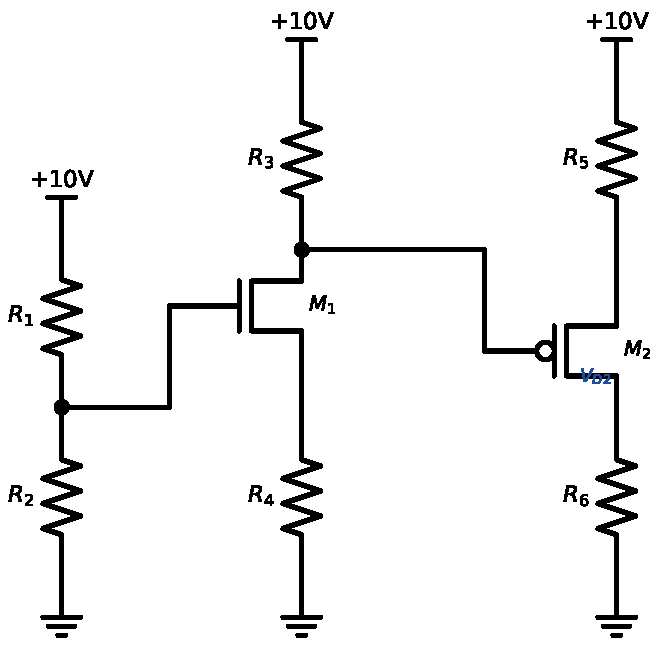
\includegraphics[width=0.9\linewidth,height=6cm,keepaspectratio]{p07_circuit}\end{center}
\solstep{1}{Rules}Run the DC analysis backwards. A target current fixes the gate--source voltage (tool T1): $V_{ov} = \sqrt{2I_D/k}$, $|V_{GS}| = |V_t| + V_{ov}$. A resistor is known as soon as the voltages at both of its ends and its current are known: $R = \Delta V/I$ ($I_G = 0$, so gate dividers carry only their own current). A mirror output copies the reference scaled by $W/L$ (tool T3). Work from the nodes that are already fixed towards the unknown ones.
\solstep{2}{Design, node by node}\begin{enumerate}[leftmargin=*,itemsep=3pt]
\item Design choice: $V_{R4} = 1$\,V across $R_{4}$: $V_{S1} = 0 + 1 = 1\,\mathrm{V}$.
\item Design choice: $V_{R5} = 2$\,V across $R_{5}$: $V_{S2} = 10 - 2 = 8\,\mathrm{V}$.
\item Design choice: the divider current is $I_{R2} = 5\,\mu \mathrm{A}$ (any value works for the bias because $I_G = 0$; it only sets the divider resistance).
\item $M_{1}$ must carry $I_{D1} = 200\,\mu \mathrm{A}$: $V_{ov1} = \sqrt{\frac{2I_{D1}}{k_{1}}} = \sqrt{\frac{2\cdot200\,\mu \mathrm{A}}{1.1\,\mathrm{m}\mathrm{A/V^2}}} = 0.603$\,V, $V_{GS1} = 1.4 + 0.603 = 2.003$\,V: $V_{G1} = V_{S1} + V_{GS1} = 3\,\mathrm{V}$.
\item $M_{2}$ must carry $I_{D2} = 500\,\mu \mathrm{A}$: $V_{ov2} = \sqrt{\frac{2I_{D2}}{k_{2}}} = \sqrt{\frac{2\cdot500\,\mu \mathrm{A}}{850\,\mu \mathrm{A/V^2}}} = 1.085$\,V, $V_{SG2} = 1.3 + 1.085 = 2.385$\,V: $V_{D1} = V_{S2} - V_{SG2} = 5.62\,\mathrm{V}$.
\item The only current through $R_{1}$ is $I_{R2} = 5\,\mu \mathrm{A}$ ($I_G = 0$).
\item $\displaystyle R_{1} = \frac{10 - V_{G1}}{I_{R2}} = \frac{10 - 3.003}{5\,\mu \mathrm{A}} = \mathbf{1.4\,\mathrm{M}\Omega}$
\item $\displaystyle R_{2} = \frac{V_{G1} - 0}{I_{R2}} = \frac{3.003 - 0}{5\,\mu \mathrm{A}} = \mathbf{601\,\mathrm{k}\Omega}$
\item The only current through $R_{3}$ is $I_{D1} = 200\,\mu \mathrm{A}$ ($I_G = 0$).
\item $\displaystyle R_{3} = \frac{10 - V_{D1}}{I_{D1}} = \frac{10 - 5.615}{200\,\mu \mathrm{A}} = \mathbf{21.9\,\mathrm{k}\Omega}$
\item The only current through $R_{4}$ is $I_{D1} = 200\,\mu \mathrm{A}$ ($I_G = 0$).
\item $\displaystyle R_{4} = \frac{V_{S1} - 0}{I_{D1}} = \frac{1 - 0}{200\,\mu \mathrm{A}} = \mathbf{5\,\mathrm{k}\Omega}$
\item The only current through $R_{5}$ is $I_{D2} = 500\,\mu \mathrm{A}$ ($I_G = 0$).
\item $\displaystyle R_{5} = \frac{10 - V_{S2}}{I_{D2}} = \frac{10 - 8}{500\,\mu \mathrm{A}} = \mathbf{4\,\mathrm{k}\Omega}$
\item The only current through $R_{6}$ is $I_{D2} = 500\,\mu \mathrm{A}$ ($I_G = 0$).
\item $\displaystyle R_{6} = \frac{V_{D2} - 0}{I_{D2}} = \frac{2 - 0}{500\,\mu \mathrm{A}} = \mathbf{4\,\mathrm{k}\Omega}$
\end{enumerate}

\solstep{3}{Designed circuit}\begin{center}\renewcommand{\arraystretch}{1.35}
\begin{tabular}{cc}
\toprule
element & value \\
\midrule
$R_{1}$ & $1.4\,\mathrm{M}\Omega$ \\
$R_{2}$ & $601\,\mathrm{k}\Omega$ \\
$R_{3}$ & $21.9\,\mathrm{k}\Omega$ \\
$R_{4}$ & $5\,\mathrm{k}\Omega$ \\
$R_{5}$ & $4\,\mathrm{k}\Omega$ \\
$R_{6}$ & $4\,\mathrm{k}\Omega$ \\
\bottomrule
\end{tabular}\end{center}
\begin{center}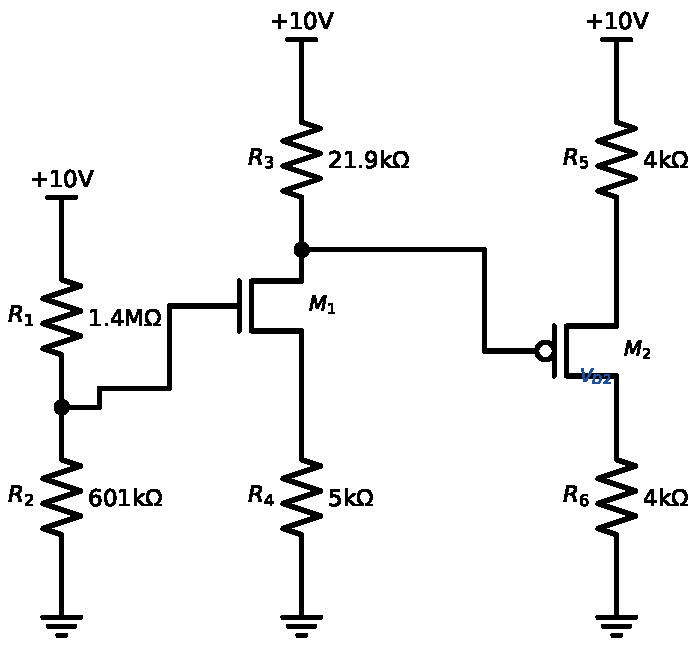
\includegraphics[width=0.85\linewidth,height=6cm,keepaspectratio]{p07_designed}\end{center}

\solstep{4}{Check by analysis}Analyse the finished circuit as in set 5A (one quadratic per transistor, mirrors by $W/L$):\begin{center}\renewcommand{\arraystretch}{1.35}
\begin{tabular}{ccc}
\toprule
 & target $I_D$ & analysis $I_D$ \\
\midrule
$M_{1}$ & $200\,\mu \mathrm{A}$ & $200\,\mu \mathrm{A}$ \\
$M_{2}$ & $500\,\mu \mathrm{A}$ & $500\,\mu \mathrm{A}$ \\
\bottomrule
\end{tabular}\end{center}
\begin{itemize}[leftmargin=*,itemsep=2pt]
\item $V_{DS1} = V_{D1} - V_{S1} = 5.615 - 1 = 4.62\,\mathrm{V}$ $\ge V_{ov1} = 0.603$\,V $\Rightarrow$ $M_{1}$ is active \checkmark
\item $V_{SD2} = V_{S2} - V_{D2} = 8 - 2 = 6\,\mathrm{V}$ $\ge V_{ov2} = 1.08$\,V $\Rightarrow$ $M_{2}$ is active \checkmark
\end{itemize}
Every specified current and voltage is reproduced exactly ($I_G = 0$: nothing was neglected).
\begin{ansbox}
$R_{1} = 1.4\,\mathrm{M}\Omega$,\quad $R_{2} = 601\,\mathrm{k}\Omega$,\quad $R_{3} = 21.9\,\mathrm{k}\Omega$,\quad $R_{4} = 5\,\mathrm{k}\Omega$,\quad $R_{5} = 4\,\mathrm{k}\Omega$,\quad $R_{6} = 4\,\mathrm{k}\Omega$
\end{ansbox}

\newpage
\subsection*{Solution 5C.8 \hfill Medium}
\begin{center}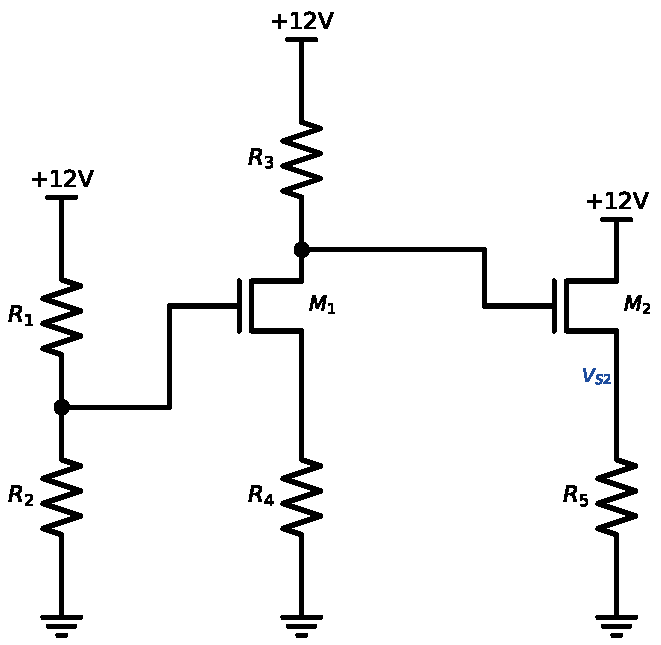
\includegraphics[width=0.9\linewidth,height=6cm,keepaspectratio]{p08_circuit}\end{center}
\solstep{1}{Rules}Run the DC analysis backwards. A target current fixes the gate--source voltage (tool T1): $V_{ov} = \sqrt{2I_D/k}$, $|V_{GS}| = |V_t| + V_{ov}$. A resistor is known as soon as the voltages at both of its ends and its current are known: $R = \Delta V/I$ ($I_G = 0$, so gate dividers carry only their own current). A mirror output copies the reference scaled by $W/L$ (tool T3). Work from the nodes that are already fixed towards the unknown ones.
\solstep{2}{Design, node by node}\begin{enumerate}[leftmargin=*,itemsep=3pt]
\item Design choice: $V_{R4} = 1$\,V across $R_{4}$: $V_{S1} = 0 + 1 = 1\,\mathrm{V}$.
\item $M_{1}$ must carry $I_{D1} = 250\,\mu \mathrm{A}$: $V_{ov1} = \sqrt{\frac{2I_{D1}}{k_{1}}} = \sqrt{\frac{2\cdot250\,\mu \mathrm{A}}{1.1\,\mathrm{m}\mathrm{A/V^2}}} = 0.6742$\,V, $V_{GS1} = 1.4 + 0.6742 = 2.074$\,V: $V_{G1} = V_{S1} + V_{GS1} = 3.07\,\mathrm{V}$.
\item $M_{2}$ must carry $I_{D2} = 1\,\mathrm{m}\mathrm{A}$: $V_{ov2} = \sqrt{\frac{2I_{D2}}{k_{2}}} = \sqrt{\frac{2\cdot1\,\mathrm{m}\mathrm{A}}{1.1\,\mathrm{m}\mathrm{A/V^2}}} = 1.348$\,V, $V_{GS2} = 1.4 + 1.348 = 2.748$\,V: $V_{D1} = V_{S2} + V_{GS2} = 7.75\,\mathrm{V}$.
\item Input-resistance requirement: $R_{1}\|R_{2} = 1\,\mathrm{M}\Omega$. Both resistors carry the same current $I$ ($I_G = 0$), so $R_{1} = V_{R1}/I = 8.926X$ and $R_{2} = 3.074X$ with $X = 1/I$. Then $R_{1}\|R_{2} = \frac{8.926\cdot3.074}{12}X = 1\,\mathrm{M}\Omega$ gives $X = 437\,\mathrm{k}\Omega$: $\mathbf{R_{1} = 3.9\,\mathrm{M}\Omega}$, $\mathbf{R_{2} = 1.34\,\mathrm{M}\Omega}$.
\item The only current through $R_{3}$ is $I_{D1} = 250\,\mu \mathrm{A}$ ($I_G = 0$).
\item $\displaystyle R_{3} = \frac{12 - V_{D1}}{I_{D1}} = \frac{12 - 7.748}{250\,\mu \mathrm{A}} = \mathbf{17\,\mathrm{k}\Omega}$
\item The only current through $R_{4}$ is $I_{D1} = 250\,\mu \mathrm{A}$ ($I_G = 0$).
\item $\displaystyle R_{4} = \frac{V_{S1} - 0}{I_{D1}} = \frac{1 - 0}{250\,\mu \mathrm{A}} = \mathbf{4\,\mathrm{k}\Omega}$
\item The only current through $R_{5}$ is $I_{D2} = 1\,\mathrm{m}\mathrm{A}$ ($I_G = 0$).
\item $\displaystyle R_{5} = \frac{V_{S2} - 0}{I_{D2}} = \frac{5 - 0}{1\,\mathrm{m}\mathrm{A}} = \mathbf{5\,\mathrm{k}\Omega}$
\end{enumerate}

\solstep{3}{Designed circuit}\begin{center}\renewcommand{\arraystretch}{1.35}
\begin{tabular}{cc}
\toprule
element & value \\
\midrule
$R_{1}$ & $3.9\,\mathrm{M}\Omega$ \\
$R_{2}$ & $1.34\,\mathrm{M}\Omega$ \\
$R_{3}$ & $17\,\mathrm{k}\Omega$ \\
$R_{4}$ & $4\,\mathrm{k}\Omega$ \\
$R_{5}$ & $5\,\mathrm{k}\Omega$ \\
\bottomrule
\end{tabular}\end{center}
\begin{center}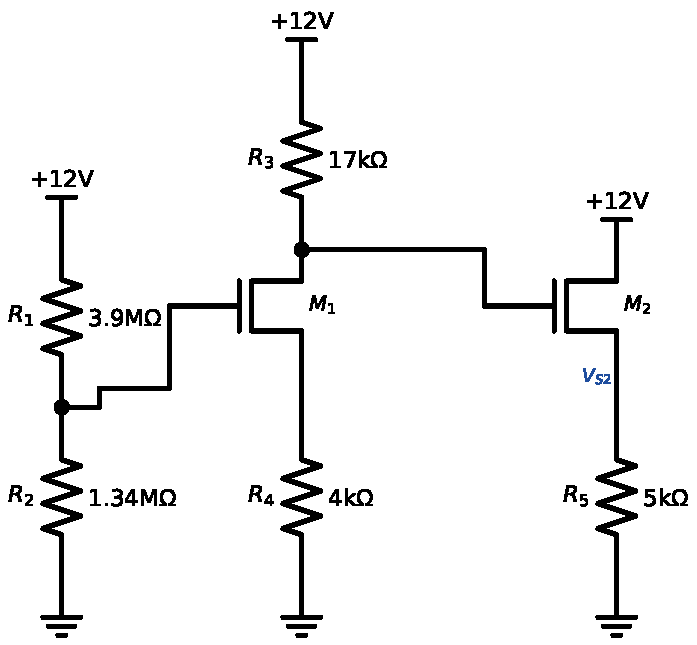
\includegraphics[width=0.85\linewidth,height=6cm,keepaspectratio]{p08_designed}\end{center}

\solstep{4}{Check by analysis}Analyse the finished circuit as in set 5A (one quadratic per transistor, mirrors by $W/L$):\begin{center}\renewcommand{\arraystretch}{1.35}
\begin{tabular}{ccc}
\toprule
 & target $I_D$ & analysis $I_D$ \\
\midrule
$M_{1}$ & $250\,\mu \mathrm{A}$ & $250\,\mu \mathrm{A}$ \\
$M_{2}$ & $1\,\mathrm{m}\mathrm{A}$ & $1\,\mathrm{m}\mathrm{A}$ \\
\bottomrule
\end{tabular}\end{center}
\begin{itemize}[leftmargin=*,itemsep=2pt]
\item $V_{DS1} = V_{D1} - V_{S1} = 7.748 - 1 = 6.75\,\mathrm{V}$ $\ge V_{ov1} = 0.674$\,V $\Rightarrow$ $M_{1}$ is active \checkmark
\item $V_{DS2} = 12 - V_{S2} = 12 - 5 = 7\,\mathrm{V}$ $\ge V_{ov2} = 1.35$\,V $\Rightarrow$ $M_{2}$ is active \checkmark
\end{itemize}
Every specified current and voltage is reproduced exactly ($I_G = 0$: nothing was neglected).
\begin{ansbox}
$R_{1} = 3.9\,\mathrm{M}\Omega$,\quad $R_{2} = 1.34\,\mathrm{M}\Omega$,\quad $R_{3} = 17\,\mathrm{k}\Omega$,\quad $R_{4} = 4\,\mathrm{k}\Omega$,\quad $R_{5} = 5\,\mathrm{k}\Omega$
\end{ansbox}

\newpage
\subsection*{Solution 5C.9 \hfill Medium}
\begin{center}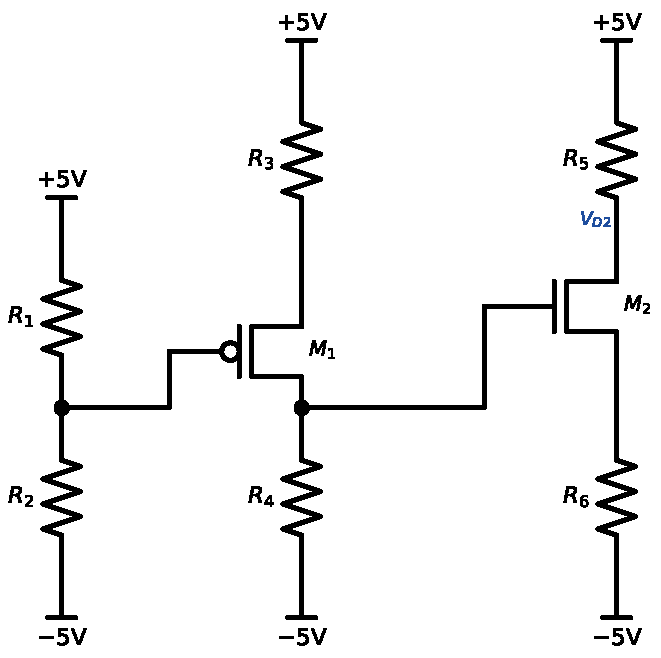
\includegraphics[width=0.9\linewidth,height=6cm,keepaspectratio]{p09_circuit}\end{center}
\solstep{1}{Rules}Run the DC analysis backwards. A target current fixes the gate--source voltage (tool T1): $V_{ov} = \sqrt{2I_D/k}$, $|V_{GS}| = |V_t| + V_{ov}$. A resistor is known as soon as the voltages at both of its ends and its current are known: $R = \Delta V/I$ ($I_G = 0$, so gate dividers carry only their own current). A mirror output copies the reference scaled by $W/L$ (tool T3). Work from the nodes that are already fixed towards the unknown ones.
\solstep{2}{Design, node by node}\begin{enumerate}[leftmargin=*,itemsep=3pt]
\item Design choice: $V_{R3} = 2$\,V across $R_{3}$: $V_{S1} = 5 - 2 = 3\,\mathrm{V}$.
\item Design choice: $V_{R6} = 1$\,V across $R_{6}$: $V_{S2} = (-5) + 1 = -4\,\mathrm{V}$.
\item Design choice: the divider current is $I_{R2} = 10\,\mu \mathrm{A}$ (any value works for the bias because $I_G = 0$; it only sets the divider resistance).
\item $M_{1}$ must carry $I_{D1} = 200\,\mu \mathrm{A}$: $V_{ov1} = \sqrt{\frac{2I_{D1}}{k_{1}}} = \sqrt{\frac{2\cdot200\,\mu \mathrm{A}}{850\,\mu \mathrm{A/V^2}}} = 0.686$\,V, $V_{SG1} = 1.3 + 0.686 = 1.986$\,V: $V_{G1} = V_{S1} - V_{SG1} = 1.01\,\mathrm{V}$.
\item $M_{2}$ must carry $I_{D2} = 400\,\mu \mathrm{A}$: $V_{ov2} = \sqrt{\frac{2I_{D2}}{k_{2}}} = \sqrt{\frac{2\cdot400\,\mu \mathrm{A}}{1.1\,\mathrm{m}\mathrm{A/V^2}}} = 0.8528$\,V, $V_{GS2} = 1.4 + 0.8528 = 2.253$\,V: $V_{D1} = V_{S2} + V_{GS2} = -1.75\,\mathrm{V}$.
\item The only current through $R_{1}$ is $I_{R2} = 10\,\mu \mathrm{A}$ ($I_G = 0$).
\item $\displaystyle R_{1} = \frac{5 - V_{G1}}{I_{R2}} = \frac{5 - 1.014}{10\,\mu \mathrm{A}} = \mathbf{399\,\mathrm{k}\Omega}$
\item $\displaystyle R_{2} = \frac{V_{G1} - (-5)}{I_{R2}} = \frac{1.014 - (-5)}{10\,\mu \mathrm{A}} = \mathbf{601\,\mathrm{k}\Omega}$
\item The only current through $R_{3}$ is $I_{D1} = 200\,\mu \mathrm{A}$ ($I_G = 0$).
\item $\displaystyle R_{3} = \frac{5 - V_{S1}}{I_{D1}} = \frac{5 - 3}{200\,\mu \mathrm{A}} = \mathbf{10\,\mathrm{k}\Omega}$
\item The only current through $R_{4}$ is $I_{D1} = 200\,\mu \mathrm{A}$ ($I_G = 0$).
\item $\displaystyle R_{4} = \frac{V_{D1} - (-5)}{I_{D1}} = \frac{-1.747 - (-5)}{200\,\mu \mathrm{A}} = \mathbf{16.3\,\mathrm{k}\Omega}$
\item The only current through $R_{5}$ is $I_{D2} = 400\,\mu \mathrm{A}$ ($I_G = 0$).
\item $\displaystyle R_{5} = \frac{5 - V_{D2}}{I_{D2}} = \frac{5 - 1}{400\,\mu \mathrm{A}} = \mathbf{10\,\mathrm{k}\Omega}$
\item The only current through $R_{6}$ is $I_{D2} = 400\,\mu \mathrm{A}$ ($I_G = 0$).
\item $\displaystyle R_{6} = \frac{V_{S2} - (-5)}{I_{D2}} = \frac{-4 - (-5)}{400\,\mu \mathrm{A}} = \mathbf{2.5\,\mathrm{k}\Omega}$
\end{enumerate}

\solstep{3}{Designed circuit}\begin{center}\renewcommand{\arraystretch}{1.35}
\begin{tabular}{cc}
\toprule
element & value \\
\midrule
$R_{1}$ & $399\,\mathrm{k}\Omega$ \\
$R_{2}$ & $601\,\mathrm{k}\Omega$ \\
$R_{3}$ & $10\,\mathrm{k}\Omega$ \\
$R_{4}$ & $16.3\,\mathrm{k}\Omega$ \\
$R_{5}$ & $10\,\mathrm{k}\Omega$ \\
$R_{6}$ & $2.5\,\mathrm{k}\Omega$ \\
\bottomrule
\end{tabular}\end{center}
\begin{center}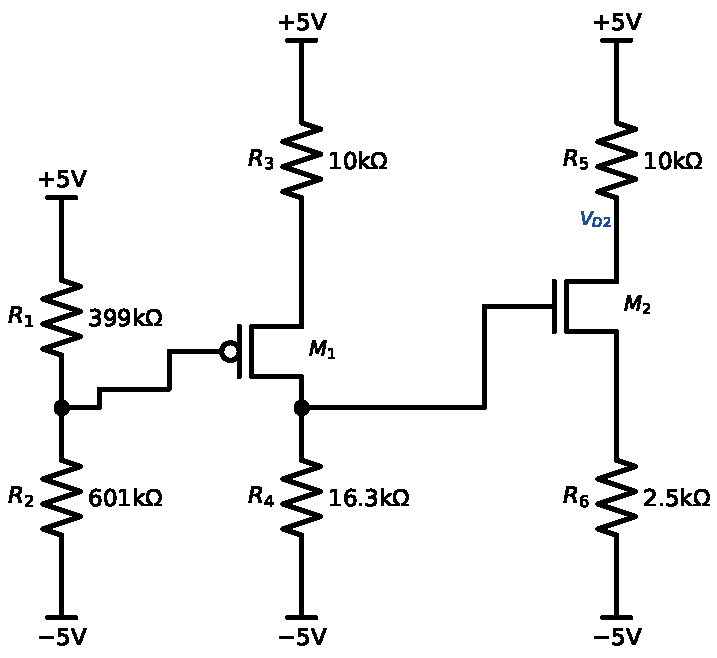
\includegraphics[width=0.85\linewidth,height=6cm,keepaspectratio]{p09_designed}\end{center}

\solstep{4}{Check by analysis}Analyse the finished circuit as in set 5A (one quadratic per transistor, mirrors by $W/L$):\begin{center}\renewcommand{\arraystretch}{1.35}
\begin{tabular}{ccc}
\toprule
 & target $I_D$ & analysis $I_D$ \\
\midrule
$M_{1}$ & $200\,\mu \mathrm{A}$ & $200\,\mu \mathrm{A}$ \\
$M_{2}$ & $400\,\mu \mathrm{A}$ & $400\,\mu \mathrm{A}$ \\
\bottomrule
\end{tabular}\end{center}
\begin{itemize}[leftmargin=*,itemsep=2pt]
\item $V_{SD1} = V_{S1} - V_{D1} = 3 - (-1.747) = 4.75\,\mathrm{V}$ $\ge V_{ov1} = 0.686$\,V $\Rightarrow$ $M_{1}$ is active \checkmark
\item $V_{DS2} = V_{D2} - V_{S2} = 1 - (-4) = 5\,\mathrm{V}$ $\ge V_{ov2} = 0.853$\,V $\Rightarrow$ $M_{2}$ is active \checkmark
\end{itemize}
Every specified current and voltage is reproduced exactly ($I_G = 0$: nothing was neglected).
\begin{ansbox}
$R_{1} = 399\,\mathrm{k}\Omega$,\quad $R_{2} = 601\,\mathrm{k}\Omega$,\quad $R_{3} = 10\,\mathrm{k}\Omega$,\quad $R_{4} = 16.3\,\mathrm{k}\Omega$,\quad $R_{5} = 10\,\mathrm{k}\Omega$,\quad $R_{6} = 2.5\,\mathrm{k}\Omega$
\end{ansbox}

\newpage
\subsection*{Solution 5C.10 \hfill Medium}
\begin{center}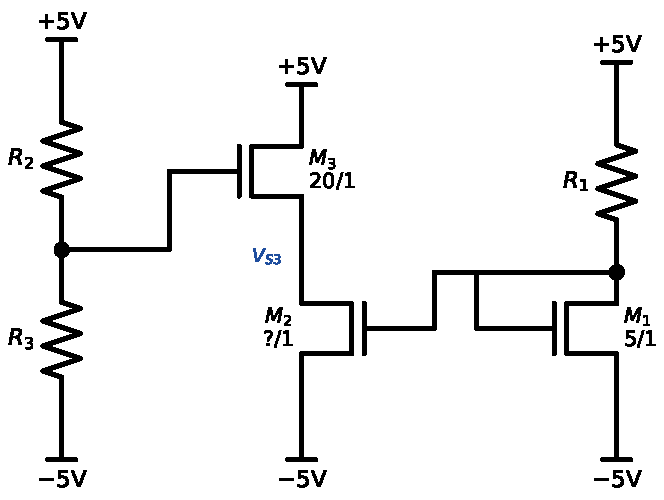
\includegraphics[width=0.9\linewidth,height=6cm,keepaspectratio]{p10_circuit}\end{center}
\solstep{1}{Rules}Run the DC analysis backwards. A target current fixes the gate--source voltage (tool T1): $V_{ov} = \sqrt{2I_D/k}$, $|V_{GS}| = |V_t| + V_{ov}$. A resistor is known as soon as the voltages at both of its ends and its current are known: $R = \Delta V/I$ ($I_G = 0$, so gate dividers carry only their own current). A mirror output copies the reference scaled by $W/L$ (tool T3). Work from the nodes that are already fixed towards the unknown ones.
\solstep{2}{Design, node by node}\begin{enumerate}[leftmargin=*,itemsep=3pt]
\item Design choice: the divider current is $I_{R3} = 5\,\mu \mathrm{A}$ (any value works for the bias because $I_G = 0$; it only sets the divider resistance).
\item $M_{2}$ shares gate and source with $M_{1}$ (same $V_{GS}$), so its current scales with $W/L$: $\left(\frac{W}{L}\right)_{2} = \frac{I_{D2}}{I_{D1}}\left(\frac{W}{L}\right)_{1} = \frac{200\,\mu \mathrm{A}}{50\,\mu \mathrm{A}}\cdot\frac{5}{1} = \mathbf{20/1}$ (keep $L = 1\,\mu$m).
\item $V_{G2} = (-5) + V_{GS2} = -3.98\,\mathrm{V}$.
\item $M_{1}$ must carry $I_{D1} = 50\,\mu \mathrm{A}$: $V_{ov1} = \sqrt{\frac{2I_{D1}}{k_{1}}} = \sqrt{\frac{2\cdot50\,\mu \mathrm{A}}{1\,\mathrm{m}\mathrm{A/V^2}}} = 0.3162$\,V, $V_{GS1} = 0.7 + 0.3162 = 1.016$\,V.
\item KCL at $V_{S3}$ ($I_G = 0$): $I_{D3} = I_{D2} = 200\,\mu \mathrm{A}$.
\item The only current through $R_{2}$ is $I_{R3} = 5\,\mu \mathrm{A}$ ($I_G = 0$).
\item $M_{3}$ must carry $I_{D3} = 200\,\mu \mathrm{A}$: $V_{ov3} = \sqrt{\frac{2I_{D3}}{k_{3}}} = \sqrt{\frac{2\cdot200\,\mu \mathrm{A}}{4\,\mathrm{m}\mathrm{A/V^2}}} = 0.3162$\,V, $V_{GS3} = 0.7 + 0.3162 = 1.016$\,V: $V_{G3} = V_{S3} + V_{GS3} = 0.0162\,\mathrm{V}$.
\item The only current through $R_{1}$ is $I_{D1} = 50\,\mu \mathrm{A}$ ($I_G = 0$).
\item $\displaystyle R_{2} = \frac{5 - V_{G3}}{I_{R3}} = \frac{5 - 0.01623}{5\,\mu \mathrm{A}} = \mathbf{997\,\mathrm{k}\Omega}$
\item $\displaystyle R_{3} = \frac{V_{G3} - (-5)}{I_{R3}} = \frac{0.01623 - (-5)}{5\,\mu \mathrm{A}} = \mathbf{1\,\mathrm{M}\Omega}$
\item $\displaystyle R_{1} = \frac{5 - V_{G2}}{I_{D1}} = \frac{5 - (-3.984)}{50\,\mu \mathrm{A}} = \mathbf{180\,\mathrm{k}\Omega}$
\end{enumerate}

\solstep{3}{Designed circuit}\begin{center}\renewcommand{\arraystretch}{1.35}
\begin{tabular}{cc}
\toprule
element & value \\
\midrule
$R_{1}$ & $180\,\mathrm{k}\Omega$ \\
$R_{2}$ & $997\,\mathrm{k}\Omega$ \\
$R_{3}$ & $1\,\mathrm{M}\Omega$ \\
$(W/L)_{2}$ & $20/1$ \\
\bottomrule
\end{tabular}\end{center}
\begin{center}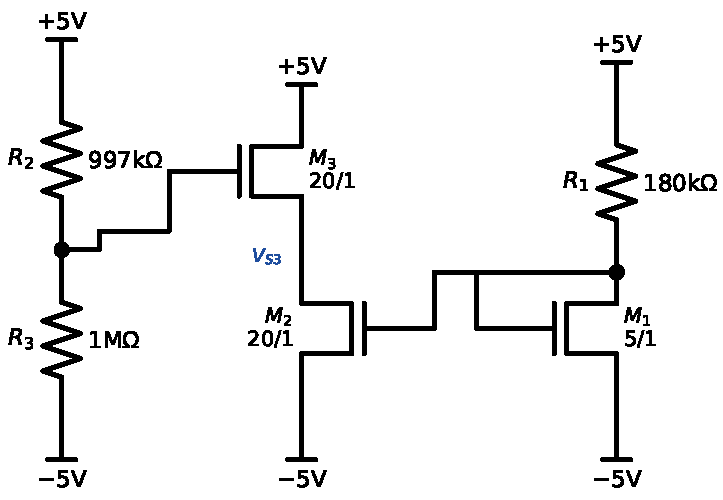
\includegraphics[width=0.85\linewidth,height=6cm,keepaspectratio]{p10_designed}\end{center}

\solstep{4}{Check by analysis}Analyse the finished circuit as in set 5A (one quadratic per transistor, mirrors by $W/L$):\begin{center}\renewcommand{\arraystretch}{1.35}
\begin{tabular}{ccc}
\toprule
 & target $I_D$ & analysis $I_D$ \\
\midrule
$M_{3}$ & --- & $200\,\mu \mathrm{A}$ \\
$M_{2}$ & $200\,\mu \mathrm{A}$ & $200\,\mu \mathrm{A}$ \\
$M_{1}$ & $50\,\mu \mathrm{A}$ & $50\,\mu \mathrm{A}$ \\
\bottomrule
\end{tabular}\end{center}
\begin{itemize}[leftmargin=*,itemsep=2pt]
\item $V_{DS3} = 5 - V_{S3} = 5 - (-1) = 6\,\mathrm{V}$ $\ge V_{ov3} = 0.316$\,V $\Rightarrow$ $M_{3}$ is active \checkmark
\item $V_{DS2} = V_{S3} - (-5) = -1 - (-5) = 4\,\mathrm{V}$ $\ge V_{ov2} = 0.316$\,V $\Rightarrow$ $M_{2}$ is active \checkmark
\item $M_{1}$ is diode-connected: $V_{DS1} = V_{GS1} > V_{ov1}$, always active \checkmark
\end{itemize}
Every specified current and voltage is reproduced exactly ($I_G = 0$: nothing was neglected).
\begin{ansbox}
$R_{1} = 180\,\mathrm{k}\Omega$,\quad $R_{2} = 997\,\mathrm{k}\Omega$,\quad $R_{3} = 1\,\mathrm{M}\Omega$,\quad $(W/L)_{2} = 20/1$
\end{ansbox}

\newpage
\subsection*{Solution 5C.11 \hfill Medium}
\begin{center}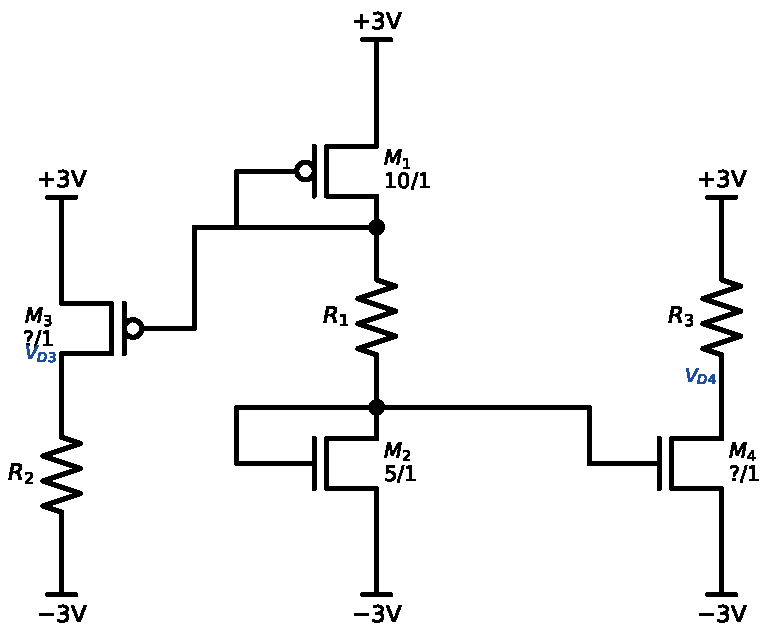
\includegraphics[width=0.9\linewidth,height=6cm,keepaspectratio]{p11_circuit}\end{center}
\solstep{1}{Rules}Run the DC analysis backwards. A target current fixes the gate--source voltage (tool T1): $V_{ov} = \sqrt{2I_D/k}$, $|V_{GS}| = |V_t| + V_{ov}$. A resistor is known as soon as the voltages at both of its ends and its current are known: $R = \Delta V/I$ ($I_G = 0$, so gate dividers carry only their own current). A mirror output copies the reference scaled by $W/L$ (tool T3). Work from the nodes that are already fixed towards the unknown ones.
\solstep{2}{Design, node by node}\begin{enumerate}[leftmargin=*,itemsep=3pt]
\item $M_{3}$ shares gate and source with $M_{1}$ (same $V_{GS}$), so its current scales with $W/L$: $\left(\frac{W}{L}\right)_{3} = \frac{I_{D3}}{I_{D1}}\left(\frac{W}{L}\right)_{1} = \frac{300\,\mu \mathrm{A}}{100\,\mu \mathrm{A}}\cdot\frac{10}{1} = \mathbf{30/1}$ (keep $L = 1\,\mu$m).
\item $V_{G3} = 3 - V_{SG3} = 1.75\,\mathrm{V}$.
\item $M_{1}$ must carry $I_{D1} = 100\,\mu \mathrm{A}$: $V_{ov1} = \sqrt{\frac{2I_{D1}}{k_{1}}} = \sqrt{\frac{2\cdot100\,\mu \mathrm{A}}{1\,\mathrm{m}\mathrm{A/V^2}}} = 0.4472$\,V, $V_{SG1} = 0.8 + 0.4472 = 1.247$\,V.
\item The only current through $R_{2}$ is $I_{D3} = 300\,\mu \mathrm{A}$ ($I_G = 0$).
\item $\displaystyle R_{2} = \frac{V_{D3} - (-3)}{I_{D3}} = \frac{0 - (-3)}{300\,\mu \mathrm{A}} = \mathbf{10\,\mathrm{k}\Omega}$
\item The only current through $R_{1}$ is $I_{D1} = 100\,\mu \mathrm{A}$ ($I_G = 0$).
\item KCL at $V_{G2}$ ($I_G = 0$): $I_{D2} = I_{D1} = 100\,\mu \mathrm{A}$.
\item The only current through $R_{3}$ is $I_{D4} = 150\,\mu \mathrm{A}$ ($I_G = 0$).
\item $\displaystyle R_{3} = \frac{3 - V_{D4}}{I_{D4}} = \frac{3 - 0.5}{150\,\mu \mathrm{A}} = \mathbf{16.7\,\mathrm{k}\Omega}$
\item $M_{4}$ shares gate and source with $M_{2}$ (same $V_{GS}$), so its current scales with $W/L$: $\left(\frac{W}{L}\right)_{4} = \frac{I_{D4}}{I_{D2}}\left(\frac{W}{L}\right)_{2} = \frac{150\,\mu \mathrm{A}}{100\,\mu \mathrm{A}}\cdot\frac{5}{1} = \mathbf{7.5/1}$ (keep $L = 1\,\mu$m).
\item $M_{2}$ must carry $I_{D2} = 100\,\mu \mathrm{A}$: $V_{ov2} = \sqrt{\frac{2I_{D2}}{k_{2}}} = \sqrt{\frac{2\cdot100\,\mu \mathrm{A}}{1\,\mathrm{m}\mathrm{A/V^2}}} = 0.4472$\,V, $V_{GS2} = 0.7 + 0.4472 = 1.147$\,V: $V_{G2} = (-3) + V_{GS2} = -1.85\,\mathrm{V}$ (diode-connected: also its drain).
\item $\displaystyle R_{1} = \frac{V_{G3} - V_{G2}}{I_{D1}} = \frac{1.753 - (-1.853)}{100\,\mu \mathrm{A}} = \mathbf{36.1\,\mathrm{k}\Omega}$
\end{enumerate}

\solstep{3}{Designed circuit}\begin{center}\renewcommand{\arraystretch}{1.35}
\begin{tabular}{cc}
\toprule
element & value \\
\midrule
$R_{1}$ & $36.1\,\mathrm{k}\Omega$ \\
$R_{2}$ & $10\,\mathrm{k}\Omega$ \\
$R_{3}$ & $16.7\,\mathrm{k}\Omega$ \\
$(W/L)_{3}$ & $30/1$ \\
$(W/L)_{4}$ & $7.5/1$ \\
\bottomrule
\end{tabular}\end{center}
\begin{center}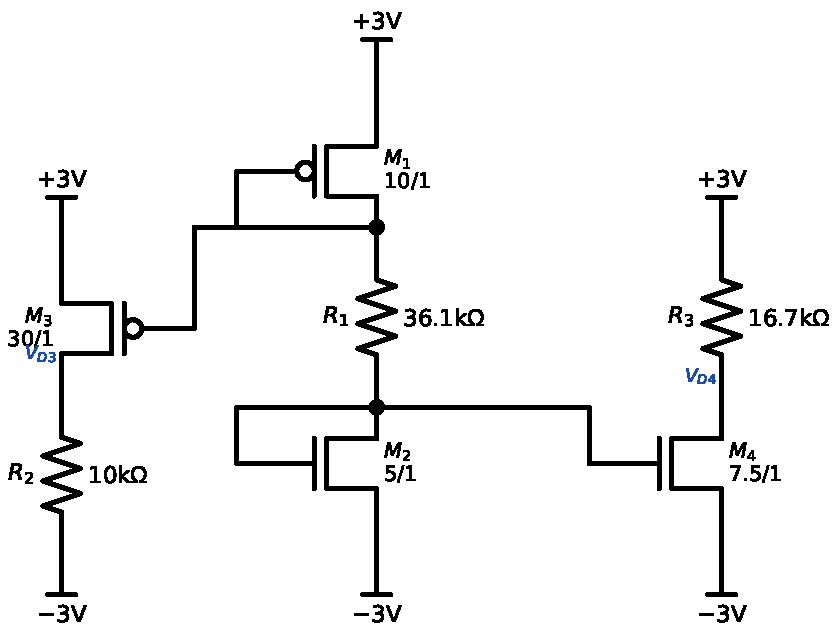
\includegraphics[width=0.85\linewidth,height=6cm,keepaspectratio]{p11_designed}\end{center}

\solstep{4}{Check by analysis}Analyse the finished circuit as in set 5A (one quadratic per transistor, mirrors by $W/L$):\begin{center}\renewcommand{\arraystretch}{1.35}
\begin{tabular}{ccc}
\toprule
 & target $I_D$ & analysis $I_D$ \\
\midrule
$M_{3}$ & $300\,\mu \mathrm{A}$ & $300\,\mu \mathrm{A}$ \\
$M_{1}$ & $100\,\mu \mathrm{A}$ & $100\,\mu \mathrm{A}$ \\
$M_{2}$ & --- & $100\,\mu \mathrm{A}$ \\
$M_{4}$ & $150\,\mu \mathrm{A}$ & $150\,\mu \mathrm{A}$ \\
\bottomrule
\end{tabular}\end{center}
\begin{itemize}[leftmargin=*,itemsep=2pt]
\item $V_{SD3} = 3 - V_{D3} = 3 - (-1.084\times 10^{-15}) = 3\,\mathrm{V}$ $\ge V_{ov3} = 0.447$\,V $\Rightarrow$ $M_{3}$ is active \checkmark
\item $M_{1}$ is diode-connected: $V_{SD1} = V_{SG1} > V_{ov1}$, always active \checkmark
\item $M_{2}$ is diode-connected: $V_{DS2} = V_{GS2} > V_{ov2}$, always active \checkmark
\item $V_{DS4} = V_{D4} - (-3) = 0.5 - (-3) = 3.5\,\mathrm{V}$ $\ge V_{ov4} = 0.447$\,V $\Rightarrow$ $M_{4}$ is active \checkmark
\end{itemize}
Every specified current and voltage is reproduced exactly ($I_G = 0$: nothing was neglected).
\begin{ansbox}
$R_{1} = 36.1\,\mathrm{k}\Omega$,\quad $R_{2} = 10\,\mathrm{k}\Omega$,\quad $R_{3} = 16.7\,\mathrm{k}\Omega$,\quad $(W/L)_{3} = 30/1$,\quad $(W/L)_{4} = 7.5/1$
\end{ansbox}

\newpage
\subsection*{Solution 5C.12 \hfill Medium}
\begin{center}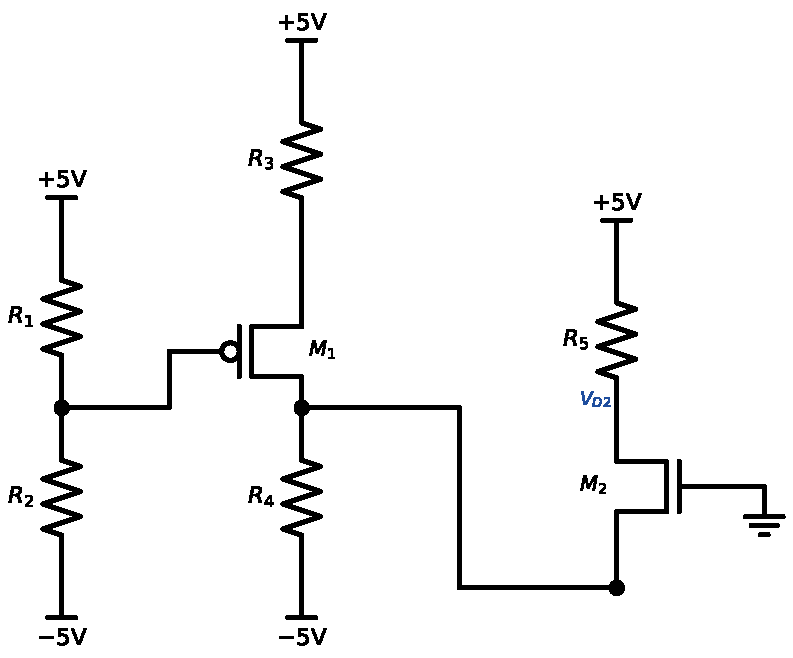
\includegraphics[width=0.9\linewidth,height=6cm,keepaspectratio]{p12_circuit}\end{center}
\solstep{1}{Rules}Run the DC analysis backwards. A target current fixes the gate--source voltage (tool T1): $V_{ov} = \sqrt{2I_D/k}$, $|V_{GS}| = |V_t| + V_{ov}$. A resistor is known as soon as the voltages at both of its ends and its current are known: $R = \Delta V/I$ ($I_G = 0$, so gate dividers carry only their own current). A mirror output copies the reference scaled by $W/L$ (tool T3). Work from the nodes that are already fixed towards the unknown ones.
\solstep{2}{Design, node by node}\begin{enumerate}[leftmargin=*,itemsep=3pt]
\item Design choice: $V_{R3} = 1.5$\,V across $R_{3}$: $V_{S1} = 5 - 1.5 = 3.5\,\mathrm{V}$.
\item Design choice: the divider current is $I_{R2} = 20\,\mu \mathrm{A}$ (any value works for the bias because $I_G = 0$; it only sets the divider resistance).
\item $M_{1}$ must carry $I_{D1} = 150\,\mu \mathrm{A}$: $V_{ov1} = \sqrt{\frac{2I_{D1}}{k_{1}}} = \sqrt{\frac{2\cdot150\,\mu \mathrm{A}}{850\,\mu \mathrm{A/V^2}}} = 0.5941$\,V, $V_{SG1} = 1.3 + 0.5941 = 1.894$\,V: $V_{G1} = V_{S1} - V_{SG1} = 1.61\,\mathrm{V}$.
\item $M_{2}$ must carry $I_{D2} = 200\,\mu \mathrm{A}$: $V_{ov2} = \sqrt{\frac{2I_{D2}}{k_{2}}} = \sqrt{\frac{2\cdot200\,\mu \mathrm{A}}{1.1\,\mathrm{m}\mathrm{A/V^2}}} = 0.603$\,V, $V_{GS2} = 1.4 + 0.603 = 2.003$\,V: $V_{D1} = 0 - V_{GS2} = -2\,\mathrm{V}$.
\item The only current through $R_{1}$ is $I_{R2} = 20\,\mu \mathrm{A}$ ($I_G = 0$).
\item $\displaystyle R_{1} = \frac{5 - V_{G1}}{I_{R2}} = \frac{5 - 1.606}{20\,\mu \mathrm{A}} = \mathbf{170\,\mathrm{k}\Omega}$
\item $\displaystyle R_{2} = \frac{V_{G1} - (-5)}{I_{R2}} = \frac{1.606 - (-5)}{20\,\mu \mathrm{A}} = \mathbf{330\,\mathrm{k}\Omega}$
\item The only current through $R_{3}$ is $I_{D1} = 150\,\mu \mathrm{A}$ ($I_G = 0$).
\item $\displaystyle R_{3} = \frac{5 - V_{S1}}{I_{D1}} = \frac{5 - 3.5}{150\,\mu \mathrm{A}} = \mathbf{10\,\mathrm{k}\Omega}$
\item KCL at $V_{D1}$: $I_{R4} = I_{D1} + I_{D2} = 350\,\mu \mathrm{A}$.
\item $\displaystyle R_{4} = \frac{V_{D1} - (-5)}{I_{R4}} = \frac{-2.003 - (-5)}{350\,\mu \mathrm{A}} = \mathbf{8.56\,\mathrm{k}\Omega}$
\item The only current through $R_{5}$ is $I_{D2} = 200\,\mu \mathrm{A}$ ($I_G = 0$).
\item $\displaystyle R_{5} = \frac{5 - V_{D2}}{I_{D2}} = \frac{5 - 2}{200\,\mu \mathrm{A}} = \mathbf{15\,\mathrm{k}\Omega}$
\end{enumerate}

\solstep{3}{Designed circuit}\begin{center}\renewcommand{\arraystretch}{1.35}
\begin{tabular}{cc}
\toprule
element & value \\
\midrule
$R_{1}$ & $170\,\mathrm{k}\Omega$ \\
$R_{2}$ & $330\,\mathrm{k}\Omega$ \\
$R_{3}$ & $10\,\mathrm{k}\Omega$ \\
$R_{4}$ & $8.56\,\mathrm{k}\Omega$ \\
$R_{5}$ & $15\,\mathrm{k}\Omega$ \\
\bottomrule
\end{tabular}\end{center}
\begin{center}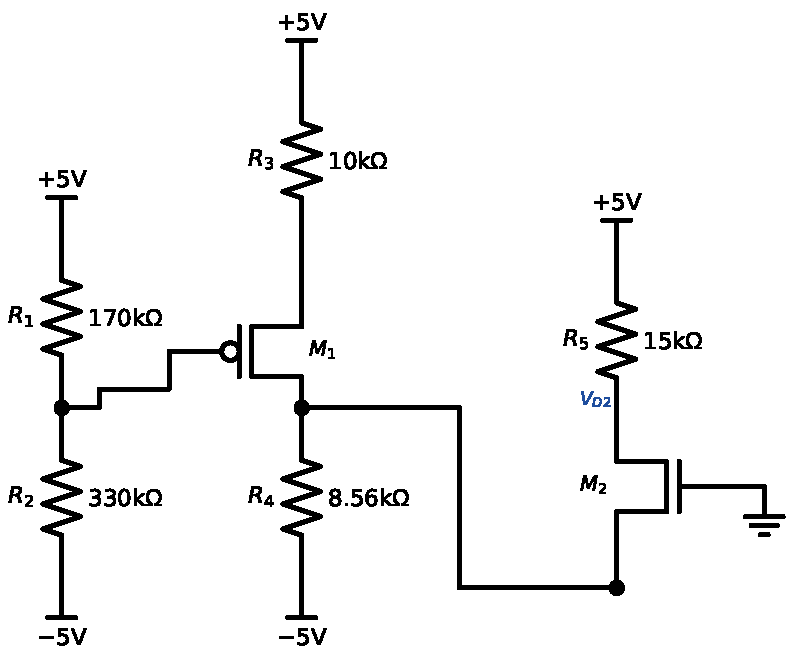
\includegraphics[width=0.85\linewidth,height=6cm,keepaspectratio]{p12_designed}\end{center}

\solstep{4}{Check by analysis}Analyse the finished circuit as in set 5A (one quadratic per transistor, mirrors by $W/L$):\begin{center}\renewcommand{\arraystretch}{1.35}
\begin{tabular}{ccc}
\toprule
 & target $I_D$ & analysis $I_D$ \\
\midrule
$M_{1}$ & $150\,\mu \mathrm{A}$ & $150\,\mu \mathrm{A}$ \\
$M_{2}$ & $200\,\mu \mathrm{A}$ & $200\,\mu \mathrm{A}$ \\
\bottomrule
\end{tabular}\end{center}
\begin{itemize}[leftmargin=*,itemsep=2pt]
\item $V_{SD1} = V_{S1} - V_{D1} = 3.5 - (-2.003) = 5.5\,\mathrm{V}$ $\ge V_{ov1} = 0.594$\,V $\Rightarrow$ $M_{1}$ is active \checkmark
\item $V_{DS2} = V_{D2} - V_{D1} = 2 - (-2.003) = 4\,\mathrm{V}$ $\ge V_{ov2} = 0.603$\,V $\Rightarrow$ $M_{2}$ is active \checkmark
\end{itemize}
Every specified current and voltage is reproduced exactly ($I_G = 0$: nothing was neglected).
\begin{ansbox}
$R_{1} = 170\,\mathrm{k}\Omega$,\quad $R_{2} = 330\,\mathrm{k}\Omega$,\quad $R_{3} = 10\,\mathrm{k}\Omega$,\quad $R_{4} = 8.56\,\mathrm{k}\Omega$,\quad $R_{5} = 15\,\mathrm{k}\Omega$
\end{ansbox}

\newpage
\subsection*{Solution 5C.13 \hfill Hard}
\begin{center}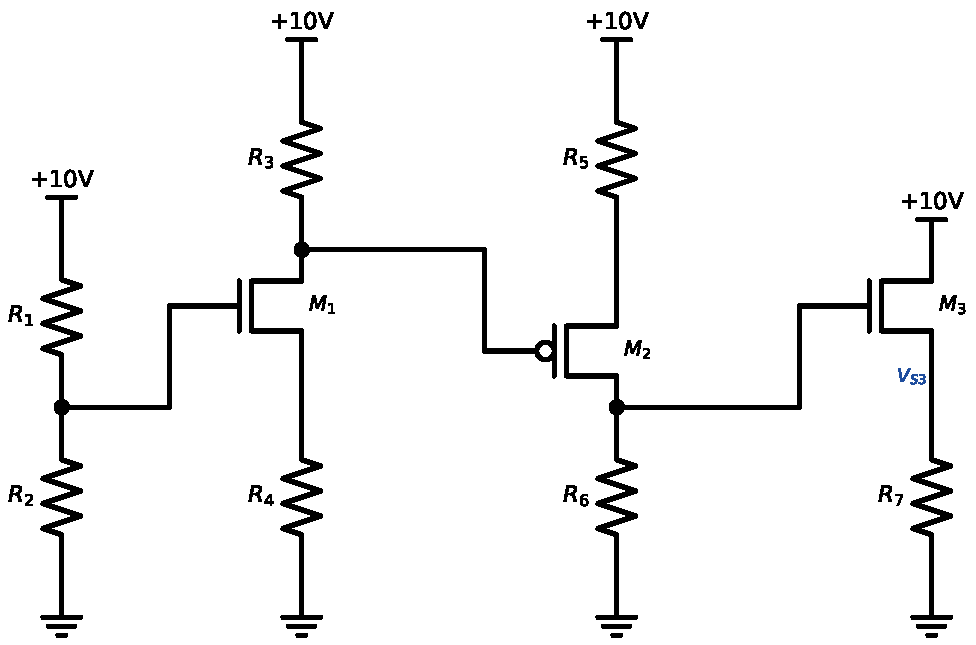
\includegraphics[width=0.9\linewidth,height=6cm,keepaspectratio]{p13_circuit}\end{center}
\solstep{1}{Rules}Run the DC analysis backwards. A target current fixes the gate--source voltage (tool T1): $V_{ov} = \sqrt{2I_D/k}$, $|V_{GS}| = |V_t| + V_{ov}$. A resistor is known as soon as the voltages at both of its ends and its current are known: $R = \Delta V/I$ ($I_G = 0$, so gate dividers carry only their own current). A mirror output copies the reference scaled by $W/L$ (tool T3). Work from the nodes that are already fixed towards the unknown ones.
\solstep{2}{Design, node by node}\begin{enumerate}[leftmargin=*,itemsep=3pt]
\item Design choice: $V_{R4} = 1$\,V across $R_{4}$: $V_{S1} = 0 + 1 = 1\,\mathrm{V}$.
\item Design choice: $V_{R5} = 2$\,V across $R_{5}$: $V_{S2} = 10 - 2 = 8\,\mathrm{V}$.
\item $M_{1}$ must carry $I_{D1} = 200\,\mu \mathrm{A}$: $V_{ov1} = \sqrt{\frac{2I_{D1}}{k_{1}}} = \sqrt{\frac{2\cdot200\,\mu \mathrm{A}}{1.1\,\mathrm{m}\mathrm{A/V^2}}} = 0.603$\,V, $V_{GS1} = 1.4 + 0.603 = 2.003$\,V: $V_{G1} = V_{S1} + V_{GS1} = 3\,\mathrm{V}$.
\item $M_{2}$ must carry $I_{D2} = 500\,\mu \mathrm{A}$: $V_{ov2} = \sqrt{\frac{2I_{D2}}{k_{2}}} = \sqrt{\frac{2\cdot500\,\mu \mathrm{A}}{850\,\mu \mathrm{A/V^2}}} = 1.085$\,V, $V_{SG2} = 1.3 + 1.085 = 2.385$\,V: $V_{D1} = V_{S2} - V_{SG2} = 5.62\,\mathrm{V}$.
\item $M_{3}$ must carry $I_{D3} = 1\,\mathrm{m}\mathrm{A}$: $V_{ov3} = \sqrt{\frac{2I_{D3}}{k_{3}}} = \sqrt{\frac{2\cdot1\,\mathrm{m}\mathrm{A}}{1.1\,\mathrm{m}\mathrm{A/V^2}}} = 1.348$\,V, $V_{GS3} = 1.4 + 1.348 = 2.748$\,V: $V_{D2} = V_{S3} + V_{GS3} = 6.75\,\mathrm{V}$.
\item Input-resistance requirement: $R_{1}\|R_{2} = 500\,\mathrm{k}\Omega$. Both resistors carry the same current $I$ ($I_G = 0$), so $R_{1} = V_{R1}/I = 6.997X$ and $R_{2} = 3.003X$ with $X = 1/I$. Then $R_{1}\|R_{2} = \frac{6.997\cdot3.003}{10}X = 500\,\mathrm{k}\Omega$ gives $X = 238\,\mathrm{k}\Omega$: $\mathbf{R_{1} = 1.66\,\mathrm{M}\Omega}$, $\mathbf{R_{2} = 715\,\mathrm{k}\Omega}$.
\item The only current through $R_{3}$ is $I_{D1} = 200\,\mu \mathrm{A}$ ($I_G = 0$).
\item $\displaystyle R_{3} = \frac{10 - V_{D1}}{I_{D1}} = \frac{10 - 5.615}{200\,\mu \mathrm{A}} = \mathbf{21.9\,\mathrm{k}\Omega}$
\item The only current through $R_{4}$ is $I_{D1} = 200\,\mu \mathrm{A}$ ($I_G = 0$).
\item $\displaystyle R_{4} = \frac{V_{S1} - 0}{I_{D1}} = \frac{1 - 0}{200\,\mu \mathrm{A}} = \mathbf{5\,\mathrm{k}\Omega}$
\item The only current through $R_{5}$ is $I_{D2} = 500\,\mu \mathrm{A}$ ($I_G = 0$).
\item $\displaystyle R_{5} = \frac{10 - V_{S2}}{I_{D2}} = \frac{10 - 8}{500\,\mu \mathrm{A}} = \mathbf{4\,\mathrm{k}\Omega}$
\item The only current through $R_{6}$ is $I_{D2} = 500\,\mu \mathrm{A}$ ($I_G = 0$).
\item $\displaystyle R_{6} = \frac{V_{D2} - 0}{I_{D2}} = \frac{6.748 - 0}{500\,\mu \mathrm{A}} = \mathbf{13.5\,\mathrm{k}\Omega}$
\item The only current through $R_{7}$ is $I_{D3} = 1\,\mathrm{m}\mathrm{A}$ ($I_G = 0$).
\item $\displaystyle R_{7} = \frac{V_{S3} - 0}{I_{D3}} = \frac{4 - 0}{1\,\mathrm{m}\mathrm{A}} = \mathbf{4\,\mathrm{k}\Omega}$
\end{enumerate}

\solstep{3}{Designed circuit}\begin{center}\renewcommand{\arraystretch}{1.35}
\begin{tabular}{cc}
\toprule
element & value \\
\midrule
$R_{1}$ & $1.66\,\mathrm{M}\Omega$ \\
$R_{2}$ & $715\,\mathrm{k}\Omega$ \\
$R_{3}$ & $21.9\,\mathrm{k}\Omega$ \\
$R_{4}$ & $5\,\mathrm{k}\Omega$ \\
$R_{5}$ & $4\,\mathrm{k}\Omega$ \\
$R_{6}$ & $13.5\,\mathrm{k}\Omega$ \\
$R_{7}$ & $4\,\mathrm{k}\Omega$ \\
\bottomrule
\end{tabular}\end{center}
\begin{center}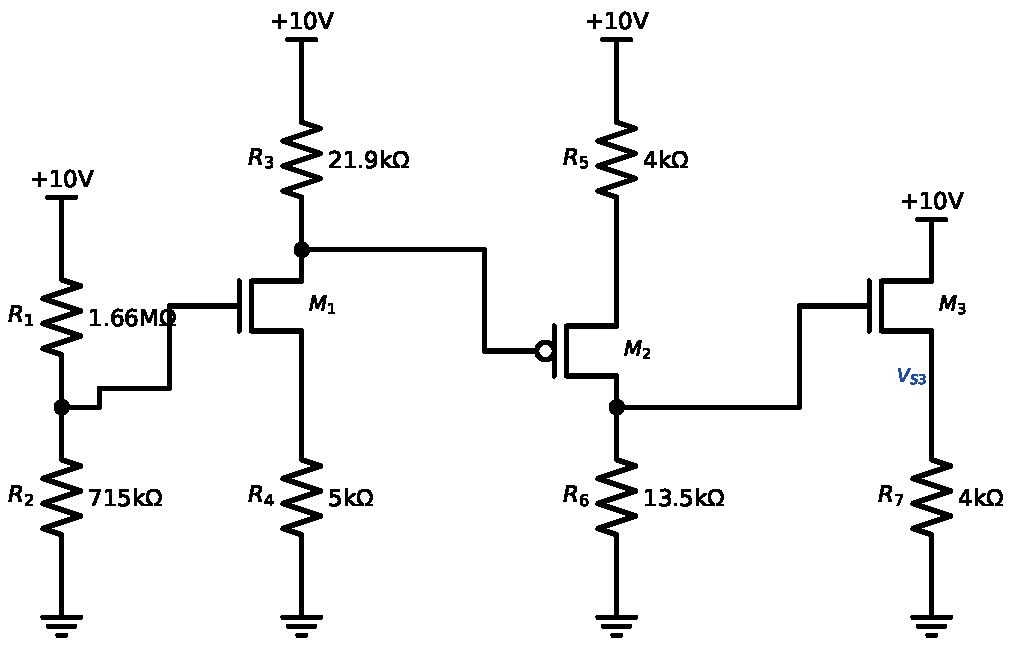
\includegraphics[width=0.85\linewidth,height=6cm,keepaspectratio]{p13_designed}\end{center}

\solstep{4}{Check by analysis}Analyse the finished circuit as in set 5A (one quadratic per transistor, mirrors by $W/L$):\begin{center}\renewcommand{\arraystretch}{1.35}
\begin{tabular}{ccc}
\toprule
 & target $I_D$ & analysis $I_D$ \\
\midrule
$M_{1}$ & $200\,\mu \mathrm{A}$ & $200\,\mu \mathrm{A}$ \\
$M_{2}$ & $500\,\mu \mathrm{A}$ & $500\,\mu \mathrm{A}$ \\
$M_{3}$ & $1\,\mathrm{m}\mathrm{A}$ & $1\,\mathrm{m}\mathrm{A}$ \\
\bottomrule
\end{tabular}\end{center}
\begin{itemize}[leftmargin=*,itemsep=2pt]
\item $V_{DS1} = V_{D1} - V_{S1} = 5.615 - 1 = 4.62\,\mathrm{V}$ $\ge V_{ov1} = 0.603$\,V $\Rightarrow$ $M_{1}$ is active \checkmark
\item $V_{SD2} = V_{S2} - V_{D2} = 8 - 6.748 = 1.25\,\mathrm{V}$ $\ge V_{ov2} = 1.08$\,V $\Rightarrow$ $M_{2}$ is active \checkmark
\item $V_{DS3} = 10 - V_{S3} = 10 - 4 = 6\,\mathrm{V}$ $\ge V_{ov3} = 1.35$\,V $\Rightarrow$ $M_{3}$ is active \checkmark
\end{itemize}
Every specified current and voltage is reproduced exactly ($I_G = 0$: nothing was neglected).
\begin{ansbox}
$R_{1} = 1.66\,\mathrm{M}\Omega$,\quad $R_{2} = 715\,\mathrm{k}\Omega$,\quad $R_{3} = 21.9\,\mathrm{k}\Omega$,\quad $R_{4} = 5\,\mathrm{k}\Omega$,\quad $R_{5} = 4\,\mathrm{k}\Omega$,\quad $R_{6} = 13.5\,\mathrm{k}\Omega$,\quad $R_{7} = 4\,\mathrm{k}\Omega$
\end{ansbox}

\newpage
\subsection*{Solution 5C.14 \hfill Hard}
\begin{center}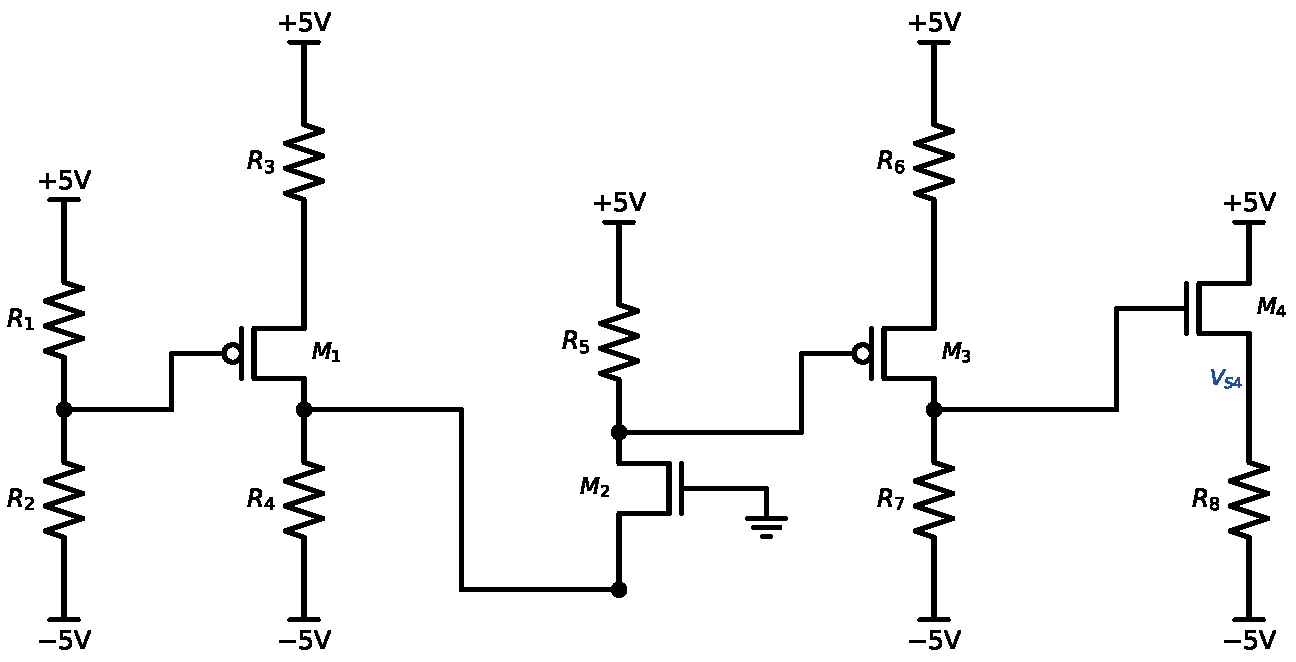
\includegraphics[width=0.9\linewidth,height=6cm,keepaspectratio]{p14_circuit}\end{center}
\solstep{1}{Rules}Run the DC analysis backwards. A target current fixes the gate--source voltage (tool T1): $V_{ov} = \sqrt{2I_D/k}$, $|V_{GS}| = |V_t| + V_{ov}$. A resistor is known as soon as the voltages at both of its ends and its current are known: $R = \Delta V/I$ ($I_G = 0$, so gate dividers carry only their own current). A mirror output copies the reference scaled by $W/L$ (tool T3). Work from the nodes that are already fixed towards the unknown ones.
\solstep{2}{Design, node by node}\begin{enumerate}[leftmargin=*,itemsep=3pt]
\item Design choice: $V_{R3} = 1.5$\,V across $R_{3}$: $V_{S1} = 5 - 1.5 = 3.5\,\mathrm{V}$.
\item Design choice: $V_{R6} = 1$\,V across $R_{6}$: $V_{S3} = 5 - 1 = 4\,\mathrm{V}$.
\item Design choice: the divider current is $I_{R2} = 20\,\mu \mathrm{A}$ (any value works for the bias because $I_G = 0$; it only sets the divider resistance).
\item $M_{1}$ must carry $I_{D1} = 100\,\mu \mathrm{A}$: $V_{ov1} = \sqrt{\frac{2I_{D1}}{k_{1}}} = \sqrt{\frac{2\cdot100\,\mu \mathrm{A}}{850\,\mu \mathrm{A/V^2}}} = 0.4851$\,V, $V_{SG1} = 1.3 + 0.4851 = 1.785$\,V: $V_{G1} = V_{S1} - V_{SG1} = 1.71\,\mathrm{V}$.
\item $M_{2}$ must carry $I_{D2} = 200\,\mu \mathrm{A}$: $V_{ov2} = \sqrt{\frac{2I_{D2}}{k_{2}}} = \sqrt{\frac{2\cdot200\,\mu \mathrm{A}}{1.1\,\mathrm{m}\mathrm{A/V^2}}} = 0.603$\,V, $V_{GS2} = 1.4 + 0.603 = 2.003$\,V: $V_{D1} = 0 - V_{GS2} = -2\,\mathrm{V}$.
\item $M_{3}$ must carry $I_{D3} = 500\,\mu \mathrm{A}$: $V_{ov3} = \sqrt{\frac{2I_{D3}}{k_{3}}} = \sqrt{\frac{2\cdot500\,\mu \mathrm{A}}{850\,\mu \mathrm{A/V^2}}} = 1.085$\,V, $V_{SG3} = 1.3 + 1.085 = 2.385$\,V: $V_{D2} = V_{S3} - V_{SG3} = 1.62\,\mathrm{V}$.
\item $M_{4}$ must carry $I_{D4} = 1\,\mathrm{m}\mathrm{A}$: $V_{ov4} = \sqrt{\frac{2I_{D4}}{k_{4}}} = \sqrt{\frac{2\cdot1\,\mathrm{m}\mathrm{A}}{1.1\,\mathrm{m}\mathrm{A/V^2}}} = 1.348$\,V, $V_{GS4} = 1.4 + 1.348 = 2.748$\,V: $V_{D3} = V_{S4} + V_{GS4} = 0.748\,\mathrm{V}$.
\item The only current through $R_{1}$ is $I_{R2} = 20\,\mu \mathrm{A}$ ($I_G = 0$).
\item $\displaystyle R_{1} = \frac{5 - V_{G1}}{I_{R2}} = \frac{5 - 1.715}{20\,\mu \mathrm{A}} = \mathbf{164\,\mathrm{k}\Omega}$
\item $\displaystyle R_{2} = \frac{V_{G1} - (-5)}{I_{R2}} = \frac{1.715 - (-5)}{20\,\mu \mathrm{A}} = \mathbf{336\,\mathrm{k}\Omega}$
\item The only current through $R_{3}$ is $I_{D1} = 100\,\mu \mathrm{A}$ ($I_G = 0$).
\item $\displaystyle R_{3} = \frac{5 - V_{S1}}{I_{D1}} = \frac{5 - 3.5}{100\,\mu \mathrm{A}} = \mathbf{15\,\mathrm{k}\Omega}$
\item KCL at $V_{D1}$: $I_{R4} = I_{D1} + I_{D2} = 300\,\mu \mathrm{A}$.
\item $\displaystyle R_{4} = \frac{V_{D1} - (-5)}{I_{R4}} = \frac{-2.003 - (-5)}{300\,\mu \mathrm{A}} = \mathbf{9.99\,\mathrm{k}\Omega}$
\item The only current through $R_{5}$ is $I_{D2} = 200\,\mu \mathrm{A}$ ($I_G = 0$).
\item $\displaystyle R_{5} = \frac{5 - V_{D2}}{I_{D2}} = \frac{5 - 1.615}{200\,\mu \mathrm{A}} = \mathbf{16.9\,\mathrm{k}\Omega}$
\item The only current through $R_{6}$ is $I_{D3} = 500\,\mu \mathrm{A}$ ($I_G = 0$).
\item $\displaystyle R_{6} = \frac{5 - V_{S3}}{I_{D3}} = \frac{5 - 4}{500\,\mu \mathrm{A}} = \mathbf{2\,\mathrm{k}\Omega}$
\item The only current through $R_{7}$ is $I_{D3} = 500\,\mu \mathrm{A}$ ($I_G = 0$).
\item $\displaystyle R_{7} = \frac{V_{D3} - (-5)}{I_{D3}} = \frac{0.7484 - (-5)}{500\,\mu \mathrm{A}} = \mathbf{11.5\,\mathrm{k}\Omega}$
\item The only current through $R_{8}$ is $I_{D4} = 1\,\mathrm{m}\mathrm{A}$ ($I_G = 0$).
\item $\displaystyle R_{8} = \frac{V_{S4} - (-5)}{I_{D4}} = \frac{-2 - (-5)}{1\,\mathrm{m}\mathrm{A}} = \mathbf{3\,\mathrm{k}\Omega}$
\end{enumerate}

\solstep{3}{Designed circuit}\begin{center}\renewcommand{\arraystretch}{1.35}
\begin{tabular}{cc}
\toprule
element & value \\
\midrule
$R_{1}$ & $164\,\mathrm{k}\Omega$ \\
$R_{2}$ & $336\,\mathrm{k}\Omega$ \\
$R_{3}$ & $15\,\mathrm{k}\Omega$ \\
$R_{4}$ & $9.99\,\mathrm{k}\Omega$ \\
$R_{5}$ & $16.9\,\mathrm{k}\Omega$ \\
$R_{6}$ & $2\,\mathrm{k}\Omega$ \\
$R_{7}$ & $11.5\,\mathrm{k}\Omega$ \\
$R_{8}$ & $3\,\mathrm{k}\Omega$ \\
\bottomrule
\end{tabular}\end{center}
\begin{center}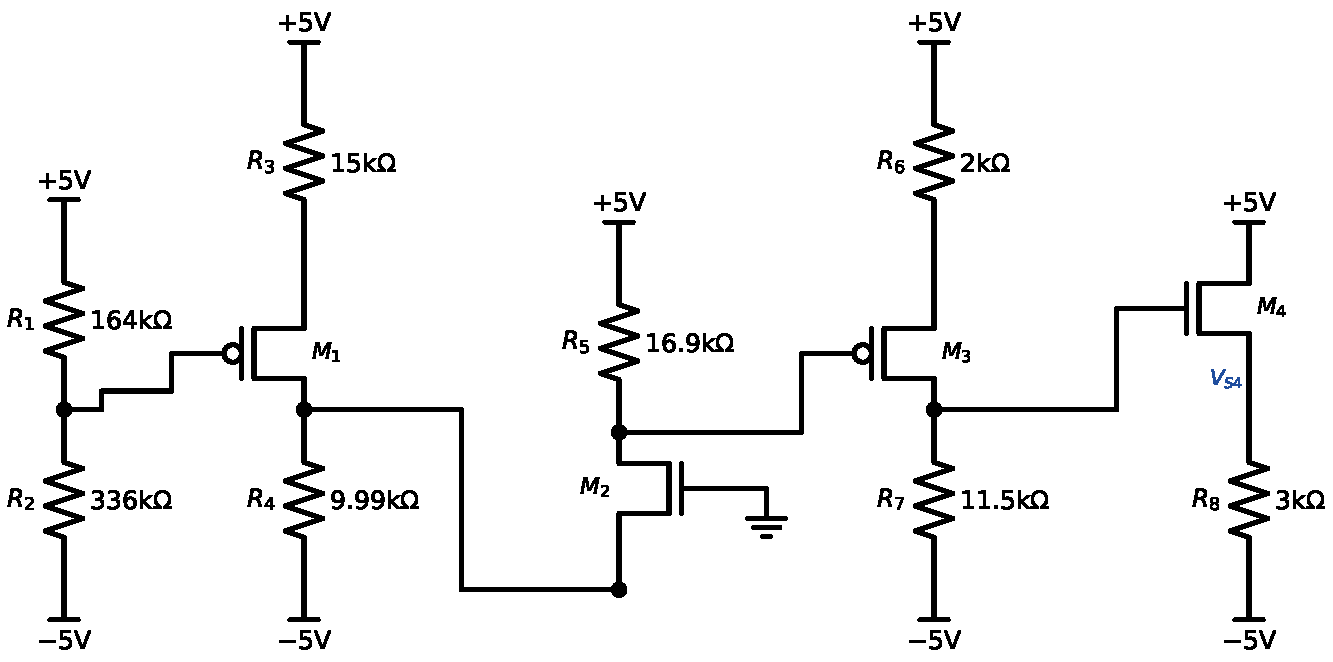
\includegraphics[width=0.85\linewidth,height=6cm,keepaspectratio]{p14_designed}\end{center}

\solstep{4}{Check by analysis}Analyse the finished circuit as in set 5A (one quadratic per transistor, mirrors by $W/L$):\begin{center}\renewcommand{\arraystretch}{1.35}
\begin{tabular}{ccc}
\toprule
 & target $I_D$ & analysis $I_D$ \\
\midrule
$M_{1}$ & $100\,\mu \mathrm{A}$ & $100\,\mu \mathrm{A}$ \\
$M_{2}$ & $200\,\mu \mathrm{A}$ & $200\,\mu \mathrm{A}$ \\
$M_{3}$ & $500\,\mu \mathrm{A}$ & $500\,\mu \mathrm{A}$ \\
$M_{4}$ & $1\,\mathrm{m}\mathrm{A}$ & $1\,\mathrm{m}\mathrm{A}$ \\
\bottomrule
\end{tabular}\end{center}
\begin{itemize}[leftmargin=*,itemsep=2pt]
\item $V_{SD1} = V_{S1} - V_{D1} = 3.5 - (-2.003) = 5.5\,\mathrm{V}$ $\ge V_{ov1} = 0.485$\,V $\Rightarrow$ $M_{1}$ is active \checkmark
\item $V_{DS2} = V_{D2} - V_{D1} = 1.615 - (-2.003) = 3.62\,\mathrm{V}$ $\ge V_{ov2} = 0.603$\,V $\Rightarrow$ $M_{2}$ is active \checkmark
\item $V_{SD3} = V_{S3} - V_{D3} = 4 - 0.7484 = 3.25\,\mathrm{V}$ $\ge V_{ov3} = 1.08$\,V $\Rightarrow$ $M_{3}$ is active \checkmark
\item $V_{DS4} = 5 - V_{S4} = 5 - (-2) = 7\,\mathrm{V}$ $\ge V_{ov4} = 1.35$\,V $\Rightarrow$ $M_{4}$ is active \checkmark
\end{itemize}
Every specified current and voltage is reproduced exactly ($I_G = 0$: nothing was neglected).
\begin{ansbox}
$R_{1} = 164\,\mathrm{k}\Omega$,\quad $R_{2} = 336\,\mathrm{k}\Omega$,\quad $R_{3} = 15\,\mathrm{k}\Omega$,\quad $R_{4} = 9.99\,\mathrm{k}\Omega$,\quad $R_{5} = 16.9\,\mathrm{k}\Omega$,\quad $R_{6} = 2\,\mathrm{k}\Omega$,\quad $R_{7} = 11.5\,\mathrm{k}\Omega$,\quad $R_{8} = 3\,\mathrm{k}\Omega$
\end{ansbox}

\newpage
\subsection*{Solution 5C.15 \hfill Hard}
\begin{center}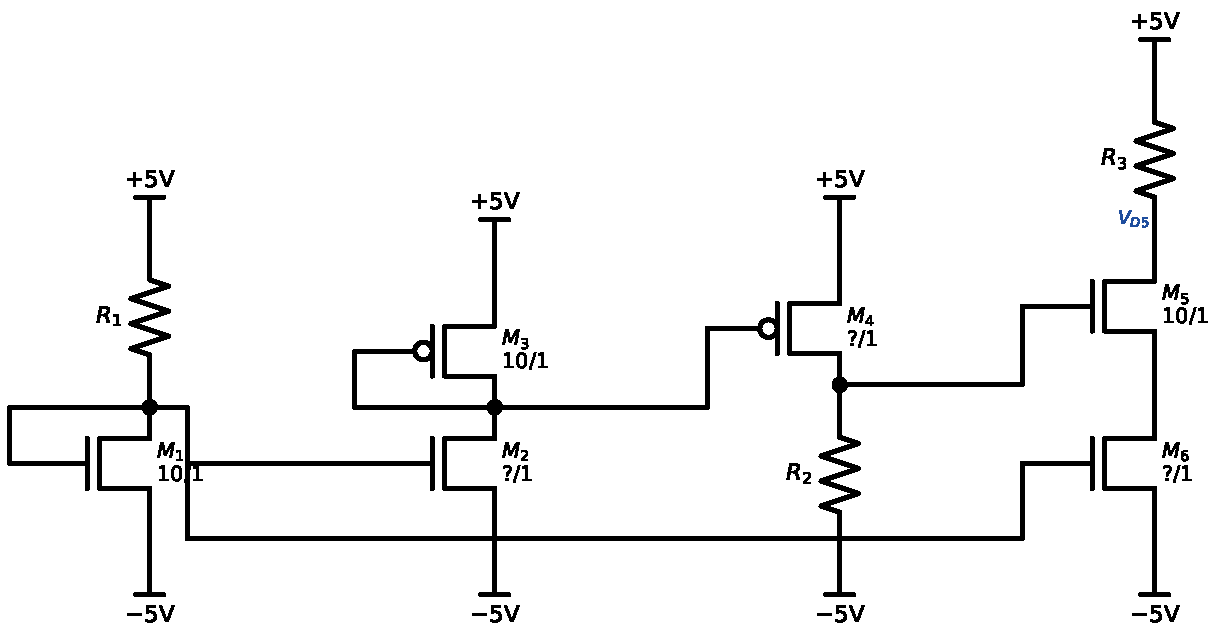
\includegraphics[width=0.9\linewidth,height=6cm,keepaspectratio]{p15_circuit}\end{center}
\solstep{1}{Rules}Run the DC analysis backwards. A target current fixes the gate--source voltage (tool T1): $V_{ov} = \sqrt{2I_D/k}$, $|V_{GS}| = |V_t| + V_{ov}$. A resistor is known as soon as the voltages at both of its ends and its current are known: $R = \Delta V/I$ ($I_G = 0$, so gate dividers carry only their own current). A mirror output copies the reference scaled by $W/L$ (tool T3). Work from the nodes that are already fixed towards the unknown ones.
\solstep{2}{Design, node by node}\begin{enumerate}[leftmargin=*,itemsep=3pt]
\item $M_{2}$ shares gate and source with $M_{1}$ (same $V_{GS}$), so its current scales with $W/L$: $\left(\frac{W}{L}\right)_{2} = \frac{I_{D2}}{I_{D1}}\left(\frac{W}{L}\right)_{1} = \frac{50\,\mu \mathrm{A}}{100\,\mu \mathrm{A}}\cdot\frac{10}{1} = \mathbf{5/1}$ (keep $L = 1\,\mu$m).
\item $M_{6}$ shares gate and source with $M_{1}$ (same $V_{GS}$), so its current scales with $W/L$: $\left(\frac{W}{L}\right)_{6} = \frac{I_{D6}}{I_{D1}}\left(\frac{W}{L}\right)_{1} = \frac{300\,\mu \mathrm{A}}{100\,\mu \mathrm{A}}\cdot\frac{10}{1} = \mathbf{30/1}$ (keep $L = 1\,\mu$m).
\item $M_{1}$ must carry $I_{D1} = 100\,\mu \mathrm{A}$: $V_{ov1} = \sqrt{\frac{2I_{D1}}{k_{1}}} = \sqrt{\frac{2\cdot100\,\mu \mathrm{A}}{2\,\mathrm{m}\mathrm{A/V^2}}} = 0.3162$\,V, $V_{GS1} = 0.7 + 0.3162 = 1.016$\,V: $V_{G1} = (-5) + V_{GS1} = -3.98\,\mathrm{V}$ (diode-connected: also its drain).
\item KCL at $V_{G3}$ ($I_G = 0$): $I_{D3} = I_{D2} = 50\,\mu \mathrm{A}$.
\item KCL at $V_{S5}$ ($I_G = 0$): $I_{D5} = I_{D6} = 300\,\mu \mathrm{A}$.
\item The only current through $R_{1}$ is $I_{D1} = 100\,\mu \mathrm{A}$ ($I_G = 0$).
\item $\displaystyle R_{1} = \frac{5 - V_{G1}}{I_{D1}} = \frac{5 - (-3.984)}{100\,\mu \mathrm{A}} = \mathbf{89.8\,\mathrm{k}\Omega}$
\item $M_{4}$ shares gate and source with $M_{3}$ (same $V_{GS}$), so its current scales with $W/L$: $\left(\frac{W}{L}\right)_{4} = \frac{I_{D4}}{I_{D3}}\left(\frac{W}{L}\right)_{3} = \frac{200\,\mu \mathrm{A}}{50\,\mu \mathrm{A}}\cdot\frac{10}{1} = \mathbf{40/1}$ (keep $L = 1\,\mu$m).
\item $M_{3}$ must carry $I_{D3} = 50\,\mu \mathrm{A}$: $V_{ov3} = \sqrt{\frac{2I_{D3}}{k_{3}}} = \sqrt{\frac{2\cdot50\,\mu \mathrm{A}}{1\,\mathrm{m}\mathrm{A/V^2}}} = 0.3162$\,V, $V_{SG3} = 0.8 + 0.3162 = 1.116$\,V: $V_{G3} = 5 - V_{SG3} = 3.88\,\mathrm{V}$ (diode-connected: also its drain).
\item $M_{5}$ must carry $I_{D5} = 300\,\mu \mathrm{A}$: $V_{ov5} = \sqrt{\frac{2I_{D5}}{k_{5}}} = \sqrt{\frac{2\cdot300\,\mu \mathrm{A}}{2\,\mathrm{m}\mathrm{A/V^2}}} = 0.5477$\,V, $V_{GS5} = 0.7 + 0.5477 = 1.248$\,V: $V_{S5} = V_{D4} - V_{GS5} = -2.25\,\mathrm{V}$.
\item The only current through $R_{2}$ is $I_{D4} = 200\,\mu \mathrm{A}$ ($I_G = 0$).
\item $\displaystyle R_{2} = \frac{V_{D4} - (-5)}{I_{D4}} = \frac{-1 - (-5)}{200\,\mu \mathrm{A}} = \mathbf{20\,\mathrm{k}\Omega}$
\item The only current through $R_{3}$ is $I_{D5} = 300\,\mu \mathrm{A}$ ($I_G = 0$).
\item $\displaystyle R_{3} = \frac{5 - V_{D5}}{I_{D5}} = \frac{5 - 2}{300\,\mu \mathrm{A}} = \mathbf{10\,\mathrm{k}\Omega}$
\end{enumerate}

\solstep{3}{Designed circuit}\begin{center}\renewcommand{\arraystretch}{1.35}
\begin{tabular}{cc}
\toprule
element & value \\
\midrule
$R_{1}$ & $89.8\,\mathrm{k}\Omega$ \\
$R_{2}$ & $20\,\mathrm{k}\Omega$ \\
$R_{3}$ & $10\,\mathrm{k}\Omega$ \\
$(W/L)_{2}$ & $5/1$ \\
$(W/L)_{4}$ & $40/1$ \\
$(W/L)_{6}$ & $30/1$ \\
\bottomrule
\end{tabular}\end{center}
\begin{center}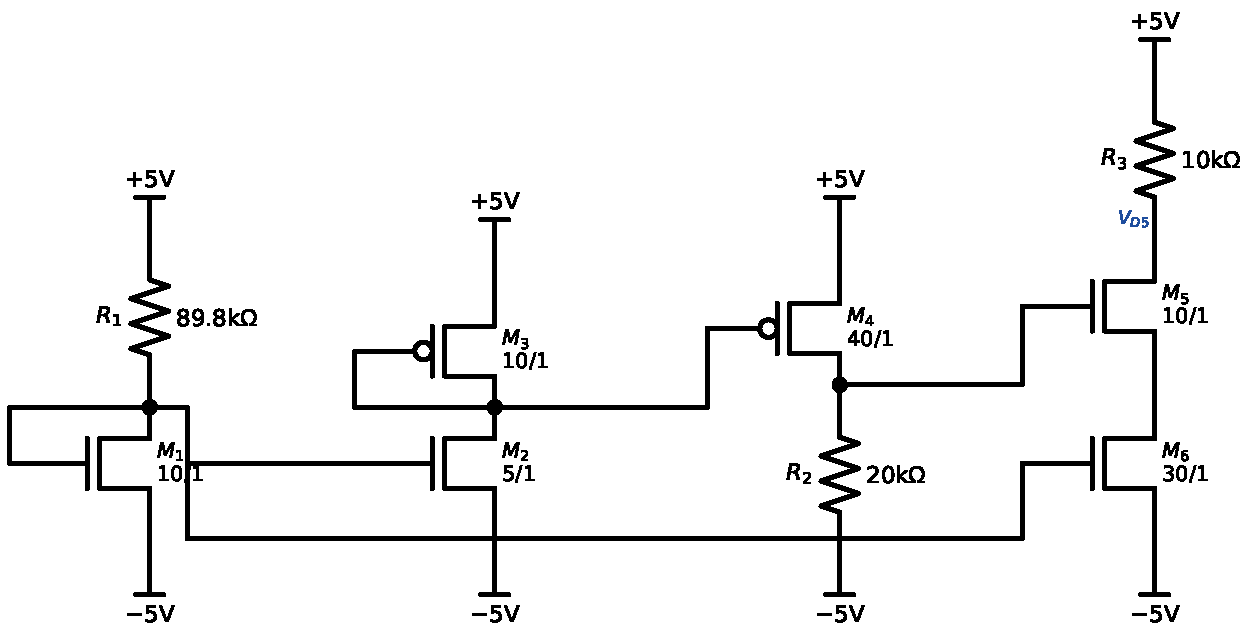
\includegraphics[width=0.85\linewidth,height=6cm,keepaspectratio]{p15_designed}\end{center}

\solstep{4}{Check by analysis}Analyse the finished circuit as in set 5A (one quadratic per transistor, mirrors by $W/L$):\begin{center}\renewcommand{\arraystretch}{1.35}
\begin{tabular}{ccc}
\toprule
 & target $I_D$ & analysis $I_D$ \\
\midrule
$M_{1}$ & $100\,\mu \mathrm{A}$ & $100\,\mu \mathrm{A}$ \\
$M_{3}$ & --- & $50\,\mu \mathrm{A}$ \\
$M_{2}$ & $50\,\mu \mathrm{A}$ & $50\,\mu \mathrm{A}$ \\
$M_{4}$ & $200\,\mu \mathrm{A}$ & $200\,\mu \mathrm{A}$ \\
$M_{5}$ & --- & $300\,\mu \mathrm{A}$ \\
$M_{6}$ & $300\,\mu \mathrm{A}$ & $300\,\mu \mathrm{A}$ \\
\bottomrule
\end{tabular}\end{center}
\begin{itemize}[leftmargin=*,itemsep=2pt]
\item $M_{1}$ is diode-connected: $V_{DS1} = V_{GS1} > V_{ov1}$, always active \checkmark
\item $M_{3}$ is diode-connected: $V_{SD3} = V_{SG3} > V_{ov3}$, always active \checkmark
\item $V_{DS2} = V_{G3} - (-5) = 3.884 - (-5) = 8.88\,\mathrm{V}$ $\ge V_{ov2} = 0.316$\,V $\Rightarrow$ $M_{2}$ is active \checkmark
\item $V_{SD4} = 5 - V_{D4} = 5 - (-1) = 6\,\mathrm{V}$ $\ge V_{ov4} = 0.316$\,V $\Rightarrow$ $M_{4}$ is active \checkmark
\item $V_{DS5} = V_{D5} - V_{S5} = 2 - (-2.248) = 4.25\,\mathrm{V}$ $\ge V_{ov5} = 0.548$\,V $\Rightarrow$ $M_{5}$ is active \checkmark
\item $V_{DS6} = V_{S5} - (-5) = -2.248 - (-5) = 2.75\,\mathrm{V}$ $\ge V_{ov6} = 0.316$\,V $\Rightarrow$ $M_{6}$ is active \checkmark
\end{itemize}
Every specified current and voltage is reproduced exactly ($I_G = 0$: nothing was neglected).
\begin{ansbox}
$R_{1} = 89.8\,\mathrm{k}\Omega$,\quad $R_{2} = 20\,\mathrm{k}\Omega$,\quad $R_{3} = 10\,\mathrm{k}\Omega$,\quad $(W/L)_{2} = 5/1$,\quad $(W/L)_{4} = 40/1$,\quad $(W/L)_{6} = 30/1$
\end{ansbox}

\newpage
\subsection*{Solution 5C.16 \hfill Hard}
\begin{center}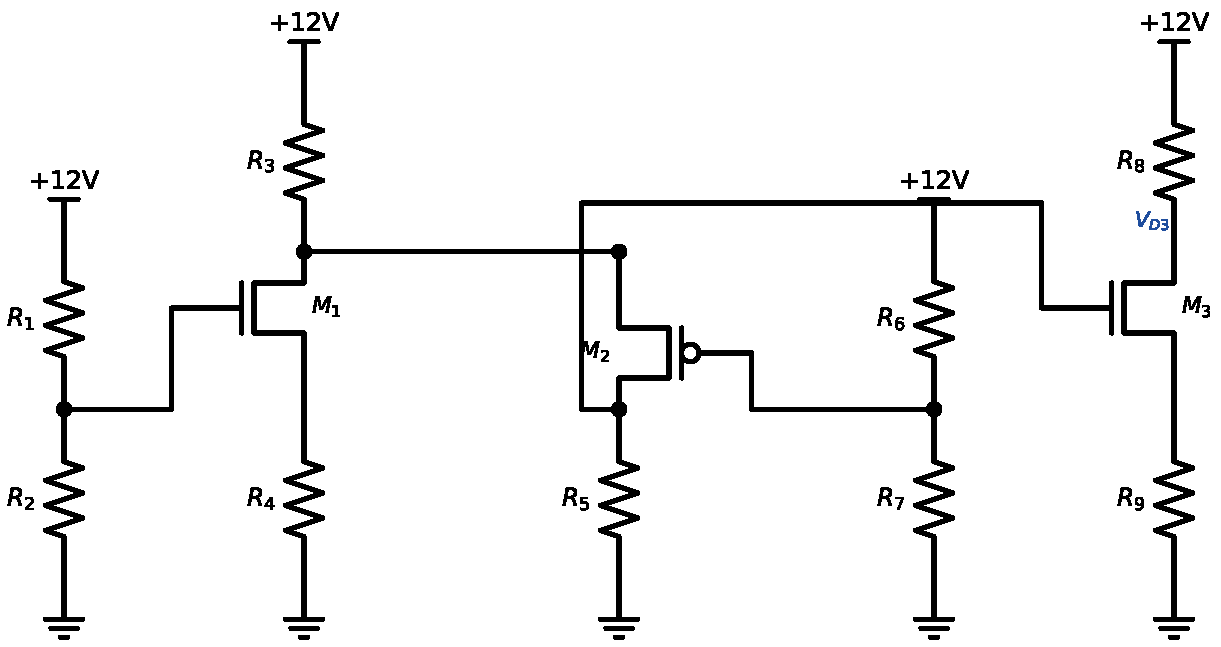
\includegraphics[width=0.9\linewidth,height=6cm,keepaspectratio]{p16_circuit}\end{center}
\solstep{1}{Rules}Run the DC analysis backwards. A target current fixes the gate--source voltage (tool T1): $V_{ov} = \sqrt{2I_D/k}$, $|V_{GS}| = |V_t| + V_{ov}$. A resistor is known as soon as the voltages at both of its ends and its current are known: $R = \Delta V/I$ ($I_G = 0$, so gate dividers carry only their own current). A mirror output copies the reference scaled by $W/L$ (tool T3). Work from the nodes that are already fixed towards the unknown ones.
\solstep{2}{Design, node by node}\begin{enumerate}[leftmargin=*,itemsep=3pt]
\item Design choice: $V_{R4} = 1$\,V across $R_{4}$: $V_{S1} = 0 + 1 = 1\,\mathrm{V}$.
\item Design choice: $V_{R9} = 1$\,V across $R_{9}$: $V_{S3} = 0 + 1 = 1\,\mathrm{V}$.
\item Design choice: the divider current is $I_{R2} = 10\,\mu \mathrm{A}$ (any value works for the bias because $I_G = 0$; it only sets the divider resistance).
\item $M_{1}$ must carry $I_{D1} = 300\,\mu \mathrm{A}$: $V_{ov1} = \sqrt{\frac{2I_{D1}}{k_{1}}} = \sqrt{\frac{2\cdot300\,\mu \mathrm{A}}{1.1\,\mathrm{m}\mathrm{A/V^2}}} = 0.7385$\,V, $V_{GS1} = 1.4 + 0.7385 = 2.139$\,V: $V_{G1} = V_{S1} + V_{GS1} = 3.14\,\mathrm{V}$.
\item $M_{2}$ must carry $I_{D2} = 200\,\mu \mathrm{A}$: $V_{ov2} = \sqrt{\frac{2I_{D2}}{k_{2}}} = \sqrt{\frac{2\cdot200\,\mu \mathrm{A}}{850\,\mu \mathrm{A/V^2}}} = 0.686$\,V, $V_{SG2} = 1.3 + 0.686 = 1.986$\,V: $V_{G2} = V_{D1} - V_{SG2} = 7.01\,\mathrm{V}$.
\item $M_{3}$ must carry $I_{D3} = 500\,\mu \mathrm{A}$: $V_{ov3} = \sqrt{\frac{2I_{D3}}{k_{3}}} = \sqrt{\frac{2\cdot500\,\mu \mathrm{A}}{1.1\,\mathrm{m}\mathrm{A/V^2}}} = 0.9535$\,V, $V_{GS3} = 1.4 + 0.9535 = 2.353$\,V: $V_{D2} = V_{S3} + V_{GS3} = 3.35\,\mathrm{V}$.
\item The only current through $R_{1}$ is $I_{R2} = 10\,\mu \mathrm{A}$ ($I_G = 0$).
\item $\displaystyle R_{1} = \frac{12 - V_{G1}}{I_{R2}} = \frac{12 - 3.139}{10\,\mu \mathrm{A}} = \mathbf{886\,\mathrm{k}\Omega}$
\item $\displaystyle R_{2} = \frac{V_{G1} - 0}{I_{R2}} = \frac{3.139 - 0}{10\,\mu \mathrm{A}} = \mathbf{314\,\mathrm{k}\Omega}$
\item Input-resistance requirement: $R_{6}\|R_{7} = 600\,\mathrm{k}\Omega$. Both resistors carry the same current $I$ ($I_G = 0$), so $R_{6} = V_{R6}/I = 4.986X$ and $R_{7} = 7.014X$ with $X = 1/I$. Then $R_{6}\|R_{7} = \frac{4.986\cdot7.014}{12}X = 600\,\mathrm{k}\Omega$ gives $X = 206\,\mathrm{k}\Omega$: $\mathbf{R_{6} = 1.03\,\mathrm{M}\Omega}$, $\mathbf{R_{7} = 1.44\,\mathrm{M}\Omega}$.
\item KCL at $V_{D1}$: $I_{R3} = I_{D1} + I_{D2} = 500\,\mu \mathrm{A}$.
\item $\displaystyle R_{3} = \frac{12 - V_{D1}}{I_{R3}} = \frac{12 - 9}{500\,\mu \mathrm{A}} = \mathbf{6\,\mathrm{k}\Omega}$
\item The only current through $R_{4}$ is $I_{D1} = 300\,\mu \mathrm{A}$ ($I_G = 0$).
\item $\displaystyle R_{4} = \frac{V_{S1} - 0}{I_{D1}} = \frac{1 - 0}{300\,\mu \mathrm{A}} = \mathbf{3.33\,\mathrm{k}\Omega}$
\item The only current through $R_{5}$ is $I_{D2} = 200\,\mu \mathrm{A}$ ($I_G = 0$).
\item $\displaystyle R_{5} = \frac{V_{D2} - 0}{I_{D2}} = \frac{3.353 - 0}{200\,\mu \mathrm{A}} = \mathbf{16.8\,\mathrm{k}\Omega}$
\item The only current through $R_{8}$ is $I_{D3} = 500\,\mu \mathrm{A}$ ($I_G = 0$).
\item $\displaystyle R_{8} = \frac{12 - V_{D3}}{I_{D3}} = \frac{12 - 6}{500\,\mu \mathrm{A}} = \mathbf{12\,\mathrm{k}\Omega}$
\item The only current through $R_{9}$ is $I_{D3} = 500\,\mu \mathrm{A}$ ($I_G = 0$).
\item $\displaystyle R_{9} = \frac{V_{S3} - 0}{I_{D3}} = \frac{1 - 0}{500\,\mu \mathrm{A}} = \mathbf{2\,\mathrm{k}\Omega}$
\end{enumerate}

\solstep{3}{Designed circuit}\begin{center}\renewcommand{\arraystretch}{1.35}
\begin{tabular}{cc}
\toprule
element & value \\
\midrule
$R_{1}$ & $886\,\mathrm{k}\Omega$ \\
$R_{2}$ & $314\,\mathrm{k}\Omega$ \\
$R_{3}$ & $6\,\mathrm{k}\Omega$ \\
$R_{4}$ & $3.33\,\mathrm{k}\Omega$ \\
$R_{5}$ & $16.8\,\mathrm{k}\Omega$ \\
$R_{6}$ & $1.03\,\mathrm{M}\Omega$ \\
$R_{7}$ & $1.44\,\mathrm{M}\Omega$ \\
$R_{8}$ & $12\,\mathrm{k}\Omega$ \\
$R_{9}$ & $2\,\mathrm{k}\Omega$ \\
\bottomrule
\end{tabular}\end{center}
\begin{center}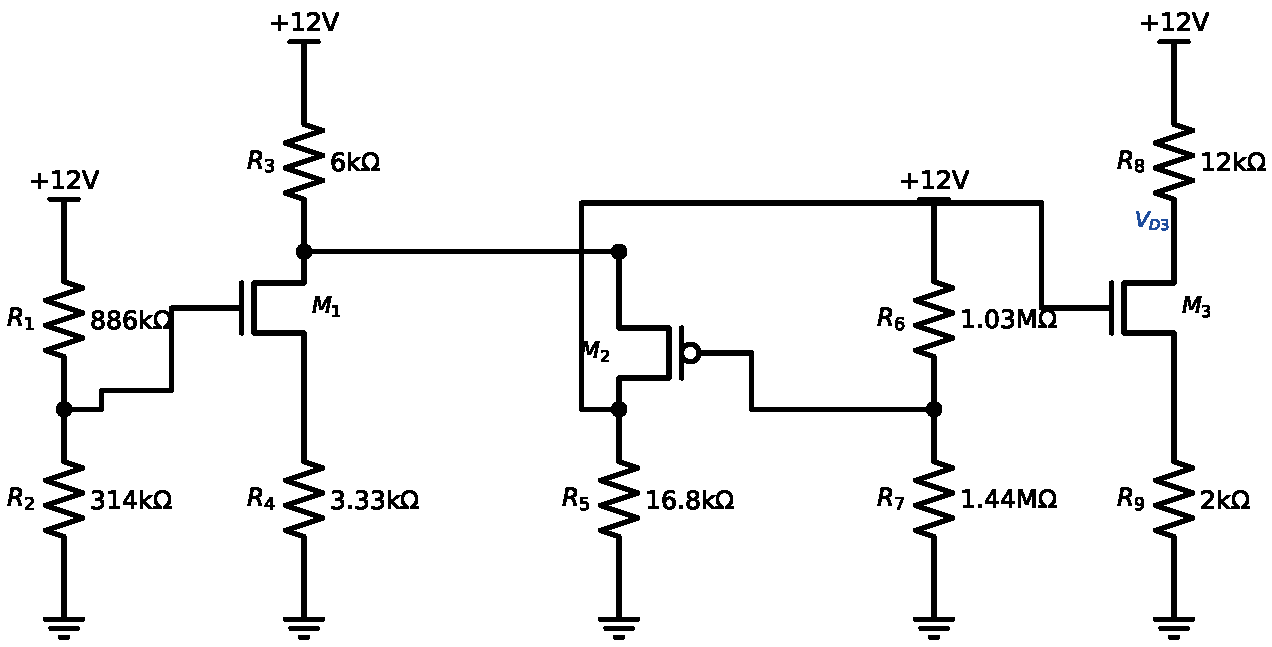
\includegraphics[width=0.85\linewidth,height=6cm,keepaspectratio]{p16_designed}\end{center}

\solstep{4}{Check by analysis}Analyse the finished circuit as in set 5A (one quadratic per transistor, mirrors by $W/L$):\begin{center}\renewcommand{\arraystretch}{1.35}
\begin{tabular}{ccc}
\toprule
 & target $I_D$ & analysis $I_D$ \\
\midrule
$M_{1}$ & $300\,\mu \mathrm{A}$ & $300\,\mu \mathrm{A}$ \\
$M_{2}$ & $200\,\mu \mathrm{A}$ & $200\,\mu \mathrm{A}$ \\
$M_{3}$ & $500\,\mu \mathrm{A}$ & $500\,\mu \mathrm{A}$ \\
\bottomrule
\end{tabular}\end{center}
\begin{itemize}[leftmargin=*,itemsep=2pt]
\item $V_{DS1} = V_{D1} - V_{S1} = 9 - 1 = 8\,\mathrm{V}$ $\ge V_{ov1} = 0.739$\,V $\Rightarrow$ $M_{1}$ is active \checkmark
\item $V_{SD2} = V_{D1} - V_{D2} = 9 - 3.353 = 5.65\,\mathrm{V}$ $\ge V_{ov2} = 0.686$\,V $\Rightarrow$ $M_{2}$ is active \checkmark
\item $V_{DS3} = V_{D3} - V_{S3} = 6 - 1 = 5\,\mathrm{V}$ $\ge V_{ov3} = 0.953$\,V $\Rightarrow$ $M_{3}$ is active \checkmark
\end{itemize}
Every specified current and voltage is reproduced exactly ($I_G = 0$: nothing was neglected).
\begin{ansbox}
$R_{1} = 886\,\mathrm{k}\Omega$,\quad $R_{2} = 314\,\mathrm{k}\Omega$,\quad $R_{3} = 6\,\mathrm{k}\Omega$,\quad $R_{4} = 3.33\,\mathrm{k}\Omega$,\quad $R_{5} = 16.8\,\mathrm{k}\Omega$,\quad $R_{6} = 1.03\,\mathrm{M}\Omega$,\quad $R_{7} = 1.44\,\mathrm{M}\Omega$,\quad $R_{8} = 12\,\mathrm{k}\Omega$,\quad $R_{9} = 2\,\mathrm{k}\Omega$
\end{ansbox}

\newpage
\subsection*{Solution 5C.17 \hfill Hard}
\begin{center}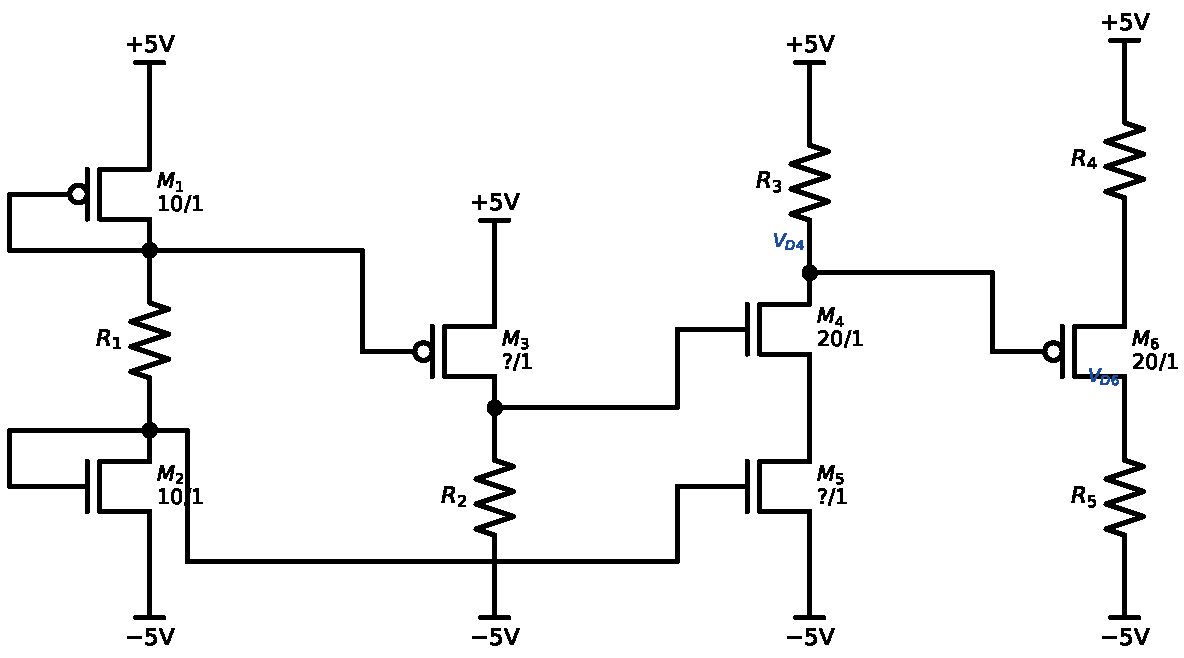
\includegraphics[width=0.9\linewidth,height=6cm,keepaspectratio]{p17_circuit}\end{center}
\solstep{1}{Rules}Run the DC analysis backwards. A target current fixes the gate--source voltage (tool T1): $V_{ov} = \sqrt{2I_D/k}$, $|V_{GS}| = |V_t| + V_{ov}$. A resistor is known as soon as the voltages at both of its ends and its current are known: $R = \Delta V/I$ ($I_G = 0$, so gate dividers carry only their own current). A mirror output copies the reference scaled by $W/L$ (tool T3). Work from the nodes that are already fixed towards the unknown ones.
\solstep{2}{Design, node by node}\begin{enumerate}[leftmargin=*,itemsep=3pt]
\item $M_{3}$ shares gate and source with $M_{1}$ (same $V_{GS}$), so its current scales with $W/L$: $\left(\frac{W}{L}\right)_{3} = \frac{I_{D3}}{I_{D1}}\left(\frac{W}{L}\right)_{1} = \frac{200\,\mu \mathrm{A}}{100\,\mu \mathrm{A}}\cdot\frac{10}{1} = \mathbf{20/1}$ (keep $L = 1\,\mu$m).
\item $M_{1}$ must carry $I_{D1} = 100\,\mu \mathrm{A}$: $V_{ov1} = \sqrt{\frac{2I_{D1}}{k_{1}}} = \sqrt{\frac{2\cdot100\,\mu \mathrm{A}}{1\,\mathrm{m}\mathrm{A/V^2}}} = 0.4472$\,V, $V_{SG1} = 0.8 + 0.4472 = 1.247$\,V: $V_{G1} = 5 - V_{SG1} = 3.75\,\mathrm{V}$ (diode-connected: also its drain).
\item $M_{6}$ must carry $I_{D6} = 300\,\mu \mathrm{A}$: $V_{ov6} = \sqrt{\frac{2I_{D6}}{k_{6}}} = \sqrt{\frac{2\cdot300\,\mu \mathrm{A}}{2\,\mathrm{m}\mathrm{A/V^2}}} = 0.5477$\,V, $V_{SG6} = 0.8 + 0.5477 = 1.348$\,V: $V_{S6} = V_{D4} + V_{SG6} = 2.35\,\mathrm{V}$.
\item KCL at $V_{S4}$ ($I_G = 0$): $I_{D4} = I_{D5} = 400\,\mu \mathrm{A}$.
\item The only current through $R_{1}$ is $I_{D1} = 100\,\mu \mathrm{A}$ ($I_G = 0$).
\item $M_{4}$ must carry $I_{D4} = 400\,\mu \mathrm{A}$: $V_{ov4} = \sqrt{\frac{2I_{D4}}{k_{4}}} = \sqrt{\frac{2\cdot400\,\mu \mathrm{A}}{4\,\mathrm{m}\mathrm{A/V^2}}} = 0.4472$\,V, $V_{GS4} = 0.7 + 0.4472 = 1.147$\,V: $V_{S4} = V_{D3} - V_{GS4} = -1.15\,\mathrm{V}$.
\item KCL at $V_{G2}$ ($I_G = 0$): $I_{D2} = I_{D1} = 100\,\mu \mathrm{A}$.
\item The only current through $R_{2}$ is $I_{D3} = 200\,\mu \mathrm{A}$ ($I_G = 0$).
\item $\displaystyle R_{2} = \frac{V_{D3} - (-5)}{I_{D3}} = \frac{0 - (-5)}{200\,\mu \mathrm{A}} = \mathbf{25\,\mathrm{k}\Omega}$
\item $M_{5}$ shares gate and source with $M_{2}$ (same $V_{GS}$), so its current scales with $W/L$: $\left(\frac{W}{L}\right)_{5} = \frac{I_{D5}}{I_{D2}}\left(\frac{W}{L}\right)_{2} = \frac{400\,\mu \mathrm{A}}{100\,\mu \mathrm{A}}\cdot\frac{10}{1} = \mathbf{40/1}$ (keep $L = 1\,\mu$m).
\item $M_{2}$ must carry $I_{D2} = 100\,\mu \mathrm{A}$: $V_{ov2} = \sqrt{\frac{2I_{D2}}{k_{2}}} = \sqrt{\frac{2\cdot100\,\mu \mathrm{A}}{2\,\mathrm{m}\mathrm{A/V^2}}} = 0.3162$\,V, $V_{GS2} = 0.7 + 0.3162 = 1.016$\,V: $V_{G2} = (-5) + V_{GS2} = -3.98\,\mathrm{V}$ (diode-connected: also its drain).
\item The only current through $R_{3}$ is $I_{D4} = 400\,\mu \mathrm{A}$ ($I_G = 0$).
\item $\displaystyle R_{1} = \frac{V_{G1} - V_{G2}}{I_{D1}} = \frac{3.753 - (-3.984)}{100\,\mu \mathrm{A}} = \mathbf{77.4\,\mathrm{k}\Omega}$
\item $\displaystyle R_{3} = \frac{5 - V_{D4}}{I_{D4}} = \frac{5 - 1}{400\,\mu \mathrm{A}} = \mathbf{10\,\mathrm{k}\Omega}$
\item The only current through $R_{4}$ is $I_{D6} = 300\,\mu \mathrm{A}$ ($I_G = 0$).
\item $\displaystyle R_{4} = \frac{5 - V_{S6}}{I_{D6}} = \frac{5 - 2.348}{300\,\mu \mathrm{A}} = \mathbf{8.84\,\mathrm{k}\Omega}$
\item The only current through $R_{5}$ is $I_{D6} = 300\,\mu \mathrm{A}$ ($I_G = 0$).
\item $\displaystyle R_{5} = \frac{V_{D6} - (-5)}{I_{D6}} = \frac{-2 - (-5)}{300\,\mu \mathrm{A}} = \mathbf{10\,\mathrm{k}\Omega}$
\end{enumerate}

\solstep{3}{Designed circuit}\begin{center}\renewcommand{\arraystretch}{1.35}
\begin{tabular}{cc}
\toprule
element & value \\
\midrule
$R_{1}$ & $77.4\,\mathrm{k}\Omega$ \\
$R_{2}$ & $25\,\mathrm{k}\Omega$ \\
$R_{3}$ & $10\,\mathrm{k}\Omega$ \\
$R_{4}$ & $8.84\,\mathrm{k}\Omega$ \\
$R_{5}$ & $10\,\mathrm{k}\Omega$ \\
$(W/L)_{3}$ & $20/1$ \\
$(W/L)_{5}$ & $40/1$ \\
\bottomrule
\end{tabular}\end{center}
\begin{center}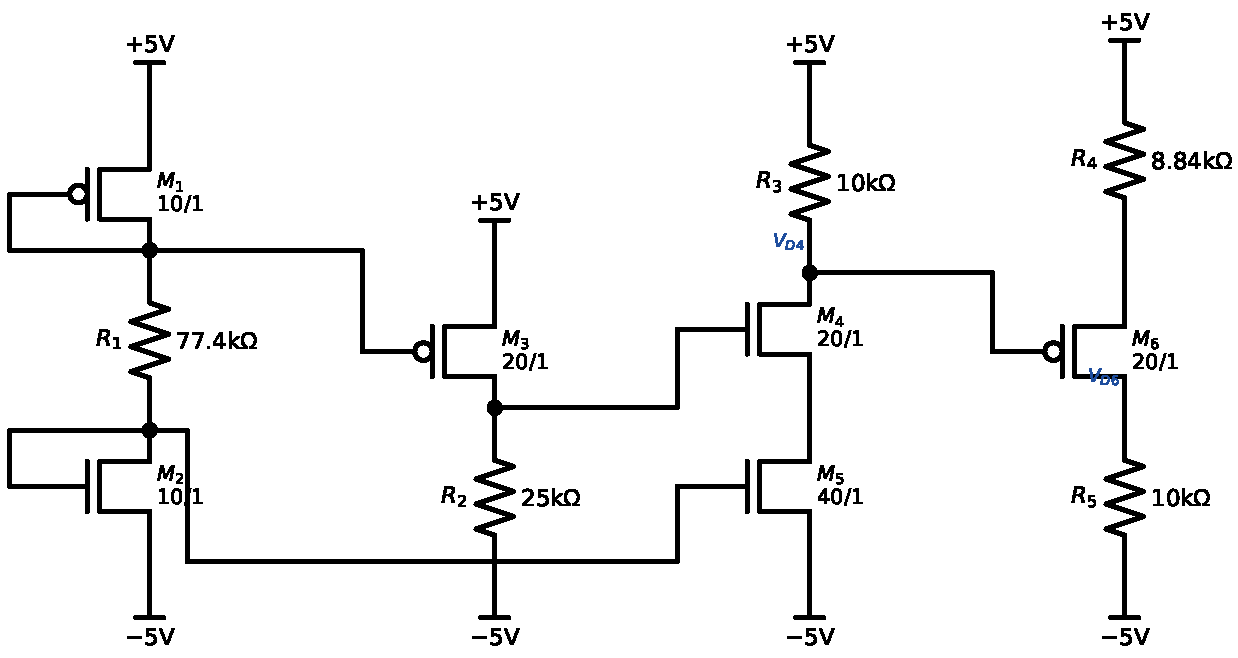
\includegraphics[width=0.85\linewidth,height=6cm,keepaspectratio]{p17_designed}\end{center}

\solstep{4}{Check by analysis}Analyse the finished circuit as in set 5A (one quadratic per transistor, mirrors by $W/L$):\begin{center}\renewcommand{\arraystretch}{1.35}
\begin{tabular}{ccc}
\toprule
 & target $I_D$ & analysis $I_D$ \\
\midrule
$M_{1}$ & $100\,\mu \mathrm{A}$ & $100\,\mu \mathrm{A}$ \\
$M_{2}$ & --- & $100\,\mu \mathrm{A}$ \\
$M_{3}$ & $200\,\mu \mathrm{A}$ & $200\,\mu \mathrm{A}$ \\
$M_{4}$ & --- & $400\,\mu \mathrm{A}$ \\
$M_{5}$ & $400\,\mu \mathrm{A}$ & $400\,\mu \mathrm{A}$ \\
$M_{6}$ & $300\,\mu \mathrm{A}$ & $300\,\mu \mathrm{A}$ \\
\bottomrule
\end{tabular}\end{center}
\begin{itemize}[leftmargin=*,itemsep=2pt]
\item $M_{1}$ is diode-connected: $V_{SD1} = V_{SG1} > V_{ov1}$, always active \checkmark
\item $M_{2}$ is diode-connected: $V_{DS2} = V_{GS2} > V_{ov2}$, always active \checkmark
\item $V_{SD3} = 5 - V_{D3} = 5 - (-6.776\times 10^{-16}) = 5\,\mathrm{V}$ $\ge V_{ov3} = 0.447$\,V $\Rightarrow$ $M_{3}$ is active \checkmark
\item $V_{DS4} = V_{D4} - V_{S4} = 1 - (-1.147) = 2.15\,\mathrm{V}$ $\ge V_{ov4} = 0.447$\,V $\Rightarrow$ $M_{4}$ is active \checkmark
\item $V_{DS5} = V_{S4} - (-5) = -1.147 - (-5) = 3.85\,\mathrm{V}$ $\ge V_{ov5} = 0.316$\,V $\Rightarrow$ $M_{5}$ is active \checkmark
\item $V_{SD6} = V_{S6} - V_{D6} = 2.348 - (-2) = 4.35\,\mathrm{V}$ $\ge V_{ov6} = 0.548$\,V $\Rightarrow$ $M_{6}$ is active \checkmark
\end{itemize}
Every specified current and voltage is reproduced exactly ($I_G = 0$: nothing was neglected).
\begin{ansbox}
$R_{1} = 77.4\,\mathrm{k}\Omega$,\quad $R_{2} = 25\,\mathrm{k}\Omega$,\quad $R_{3} = 10\,\mathrm{k}\Omega$,\quad $R_{4} = 8.84\,\mathrm{k}\Omega$,\quad $R_{5} = 10\,\mathrm{k}\Omega$,\quad $(W/L)_{3} = 20/1$,\quad $(W/L)_{5} = 40/1$
\end{ansbox}

\newpage
\subsection*{Solution 5C.18 \hfill Hard}
\begin{center}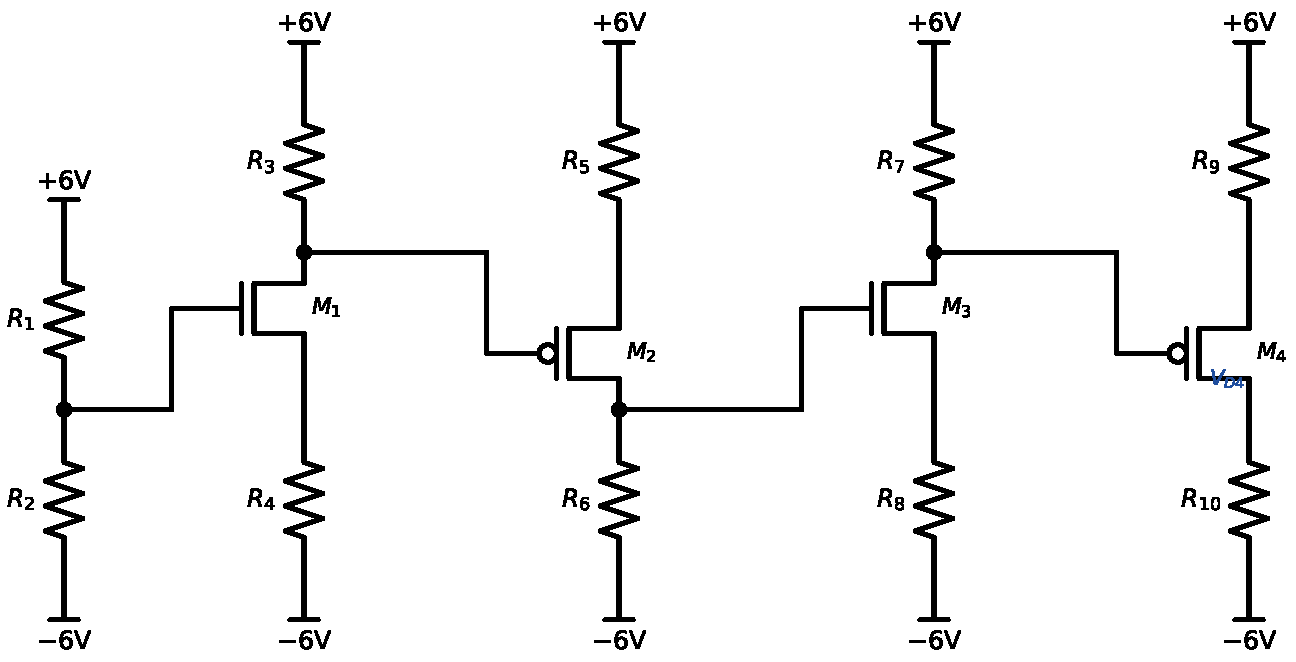
\includegraphics[width=0.9\linewidth,height=6cm,keepaspectratio]{p18_circuit}\end{center}
\solstep{1}{Rules}Run the DC analysis backwards. A target current fixes the gate--source voltage (tool T1): $V_{ov} = \sqrt{2I_D/k}$, $|V_{GS}| = |V_t| + V_{ov}$. A resistor is known as soon as the voltages at both of its ends and its current are known: $R = \Delta V/I$ ($I_G = 0$, so gate dividers carry only their own current). A mirror output copies the reference scaled by $W/L$ (tool T3). Work from the nodes that are already fixed towards the unknown ones.
\solstep{2}{Design, node by node}\begin{enumerate}[leftmargin=*,itemsep=3pt]
\item Design choice: $V_{R4} = 1$\,V across $R_{4}$: $V_{S1} = (-6) + 1 = -5\,\mathrm{V}$.
\item Design choice: $V_{R5} = 1.5$\,V across $R_{5}$: $V_{S2} = 6 - 1.5 = 4.5\,\mathrm{V}$.
\item Design choice: $V_{R8} = 1$\,V across $R_{8}$: $V_{S3} = (-6) + 1 = -5\,\mathrm{V}$.
\item Design choice: $V_{R9} = 1.5$\,V across $R_{9}$: $V_{S4} = 6 - 1.5 = 4.5\,\mathrm{V}$.
\item Design choice: the divider current is $I_{R2} = 10\,\mu \mathrm{A}$ (any value works for the bias because $I_G = 0$; it only sets the divider resistance).
\item $M_{1}$ must carry $I_{D1} = 200\,\mu \mathrm{A}$: $V_{ov1} = \sqrt{\frac{2I_{D1}}{k_{1}}} = \sqrt{\frac{2\cdot200\,\mu \mathrm{A}}{1.1\,\mathrm{m}\mathrm{A/V^2}}} = 0.603$\,V, $V_{GS1} = 1.4 + 0.603 = 2.003$\,V: $V_{G1} = V_{S1} + V_{GS1} = -3\,\mathrm{V}$.
\item $M_{2}$ must carry $I_{D2} = 300\,\mu \mathrm{A}$: $V_{ov2} = \sqrt{\frac{2I_{D2}}{k_{2}}} = \sqrt{\frac{2\cdot300\,\mu \mathrm{A}}{850\,\mu \mathrm{A/V^2}}} = 0.8402$\,V, $V_{SG2} = 1.3 + 0.8402 = 2.14$\,V: $V_{D1} = V_{S2} - V_{SG2} = 2.36\,\mathrm{V}$.
\item $M_{3}$ must carry $I_{D3} = 500\,\mu \mathrm{A}$: $V_{ov3} = \sqrt{\frac{2I_{D3}}{k_{3}}} = \sqrt{\frac{2\cdot500\,\mu \mathrm{A}}{1.1\,\mathrm{m}\mathrm{A/V^2}}} = 0.9535$\,V, $V_{GS3} = 1.4 + 0.9535 = 2.353$\,V: $V_{D2} = V_{S3} + V_{GS3} = -2.65\,\mathrm{V}$.
\item $M_{4}$ must carry $I_{D4} = 800\,\mu \mathrm{A}$: $V_{ov4} = \sqrt{\frac{2I_{D4}}{k_{4}}} = \sqrt{\frac{2\cdot800\,\mu \mathrm{A}}{850\,\mu \mathrm{A/V^2}}} = 1.372$\,V, $V_{SG4} = 1.3 + 1.372 = 2.672$\,V: $V_{D3} = V_{S4} - V_{SG4} = 1.83\,\mathrm{V}$.
\item The only current through $R_{1}$ is $I_{R2} = 10\,\mu \mathrm{A}$ ($I_G = 0$).
\item $\displaystyle R_{1} = \frac{6 - V_{G1}}{I_{R2}} = \frac{6 - (-2.997)}{10\,\mu \mathrm{A}} = \mathbf{900\,\mathrm{k}\Omega}$
\item $\displaystyle R_{2} = \frac{V_{G1} - (-6)}{I_{R2}} = \frac{-2.997 - (-6)}{10\,\mu \mathrm{A}} = \mathbf{300\,\mathrm{k}\Omega}$
\item The only current through $R_{3}$ is $I_{D1} = 200\,\mu \mathrm{A}$ ($I_G = 0$).
\item $\displaystyle R_{3} = \frac{6 - V_{D1}}{I_{D1}} = \frac{6 - 2.36}{200\,\mu \mathrm{A}} = \mathbf{18.2\,\mathrm{k}\Omega}$
\item The only current through $R_{4}$ is $I_{D1} = 200\,\mu \mathrm{A}$ ($I_G = 0$).
\item $\displaystyle R_{4} = \frac{V_{S1} - (-6)}{I_{D1}} = \frac{-5 - (-6)}{200\,\mu \mathrm{A}} = \mathbf{5\,\mathrm{k}\Omega}$
\item The only current through $R_{5}$ is $I_{D2} = 300\,\mu \mathrm{A}$ ($I_G = 0$).
\item $\displaystyle R_{5} = \frac{6 - V_{S2}}{I_{D2}} = \frac{6 - 4.5}{300\,\mu \mathrm{A}} = \mathbf{5\,\mathrm{k}\Omega}$
\item The only current through $R_{6}$ is $I_{D2} = 300\,\mu \mathrm{A}$ ($I_G = 0$).
\item $\displaystyle R_{6} = \frac{V_{D2} - (-6)}{I_{D2}} = \frac{-2.647 - (-6)}{300\,\mu \mathrm{A}} = \mathbf{11.2\,\mathrm{k}\Omega}$
\item The only current through $R_{7}$ is $I_{D3} = 500\,\mu \mathrm{A}$ ($I_G = 0$).
\item $\displaystyle R_{7} = \frac{6 - V_{D3}}{I_{D3}} = \frac{6 - 1.828}{500\,\mu \mathrm{A}} = \mathbf{8.34\,\mathrm{k}\Omega}$
\item The only current through $R_{8}$ is $I_{D3} = 500\,\mu \mathrm{A}$ ($I_G = 0$).
\item $\displaystyle R_{8} = \frac{V_{S3} - (-6)}{I_{D3}} = \frac{-5 - (-6)}{500\,\mu \mathrm{A}} = \mathbf{2\,\mathrm{k}\Omega}$
\item The only current through $R_{9}$ is $I_{D4} = 800\,\mu \mathrm{A}$ ($I_G = 0$).
\item $\displaystyle R_{9} = \frac{6 - V_{S4}}{I_{D4}} = \frac{6 - 4.5}{800\,\mu \mathrm{A}} = \mathbf{1.88\,\mathrm{k}\Omega}$
\item The only current through $R_{10}$ is $I_{D4} = 800\,\mu \mathrm{A}$ ($I_G = 0$).
\item $\displaystyle R_{10} = \frac{V_{D4} - (-6)}{I_{D4}} = \frac{-3 - (-6)}{800\,\mu \mathrm{A}} = \mathbf{3.75\,\mathrm{k}\Omega}$
\end{enumerate}

\solstep{3}{Designed circuit}\begin{center}\renewcommand{\arraystretch}{1.35}
\begin{tabular}{cc}
\toprule
element & value \\
\midrule
$R_{1}$ & $900\,\mathrm{k}\Omega$ \\
$R_{2}$ & $300\,\mathrm{k}\Omega$ \\
$R_{3}$ & $18.2\,\mathrm{k}\Omega$ \\
$R_{4}$ & $5\,\mathrm{k}\Omega$ \\
$R_{5}$ & $5\,\mathrm{k}\Omega$ \\
$R_{6}$ & $11.2\,\mathrm{k}\Omega$ \\
$R_{7}$ & $8.34\,\mathrm{k}\Omega$ \\
$R_{8}$ & $2\,\mathrm{k}\Omega$ \\
$R_{9}$ & $1.88\,\mathrm{k}\Omega$ \\
$R_{10}$ & $3.75\,\mathrm{k}\Omega$ \\
\bottomrule
\end{tabular}\end{center}
\begin{center}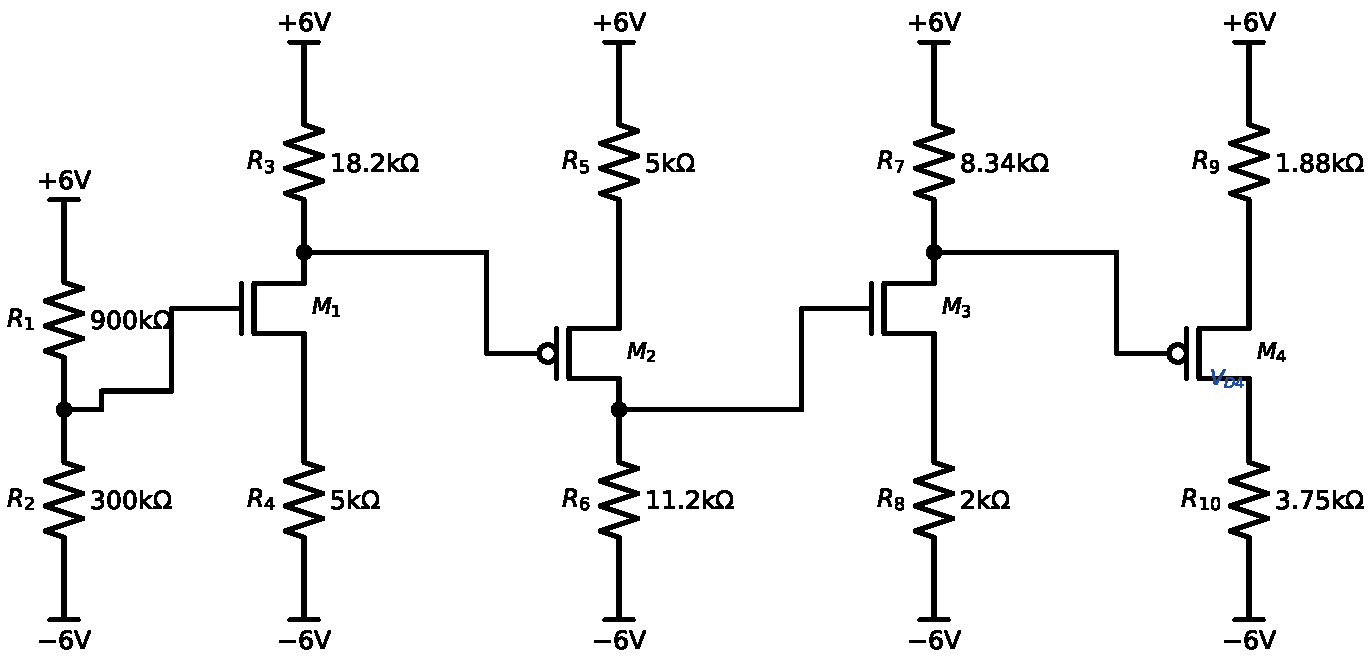
\includegraphics[width=0.85\linewidth,height=6cm,keepaspectratio]{p18_designed}\end{center}

\solstep{4}{Check by analysis}Analyse the finished circuit as in set 5A (one quadratic per transistor, mirrors by $W/L$):\begin{center}\renewcommand{\arraystretch}{1.35}
\begin{tabular}{ccc}
\toprule
 & target $I_D$ & analysis $I_D$ \\
\midrule
$M_{1}$ & $200\,\mu \mathrm{A}$ & $200\,\mu \mathrm{A}$ \\
$M_{2}$ & $300\,\mu \mathrm{A}$ & $300\,\mu \mathrm{A}$ \\
$M_{3}$ & $500\,\mu \mathrm{A}$ & $500\,\mu \mathrm{A}$ \\
$M_{4}$ & $800\,\mu \mathrm{A}$ & $800\,\mu \mathrm{A}$ \\
\bottomrule
\end{tabular}\end{center}
\begin{itemize}[leftmargin=*,itemsep=2pt]
\item $V_{DS1} = V_{D1} - V_{S1} = 2.36 - (-5) = 7.36\,\mathrm{V}$ $\ge V_{ov1} = 0.603$\,V $\Rightarrow$ $M_{1}$ is active \checkmark
\item $V_{SD2} = V_{S2} - V_{D2} = 4.5 - (-2.647) = 7.15\,\mathrm{V}$ $\ge V_{ov2} = 0.84$\,V $\Rightarrow$ $M_{2}$ is active \checkmark
\item $V_{DS3} = V_{D3} - V_{S3} = 1.828 - (-5) = 6.83\,\mathrm{V}$ $\ge V_{ov3} = 0.953$\,V $\Rightarrow$ $M_{3}$ is active \checkmark
\item $V_{SD4} = V_{S4} - V_{D4} = 4.5 - (-3) = 7.5\,\mathrm{V}$ $\ge V_{ov4} = 1.37$\,V $\Rightarrow$ $M_{4}$ is active \checkmark
\end{itemize}
Every specified current and voltage is reproduced exactly ($I_G = 0$: nothing was neglected).
\begin{ansbox}
$R_{1} = 900\,\mathrm{k}\Omega$,\quad $R_{2} = 300\,\mathrm{k}\Omega$,\quad $R_{3} = 18.2\,\mathrm{k}\Omega$,\quad $R_{4} = 5\,\mathrm{k}\Omega$,\quad $R_{5} = 5\,\mathrm{k}\Omega$,\quad $R_{6} = 11.2\,\mathrm{k}\Omega$,\quad $R_{7} = 8.34\,\mathrm{k}\Omega$,\quad $R_{8} = 2\,\mathrm{k}\Omega$,\quad $R_{9} = 1.88\,\mathrm{k}\Omega$,\quad $R_{10} = 3.75\,\mathrm{k}\Omega$
\end{ansbox}

\end{document}
